%==============================================%
%					       %
%	      <<LaTeX Source Code>>	       %
%					       %
%		 Nick Miladinovic		       %
%					       %
%	Dept. of Physics and Astronomy	       %
%		  McMaster Uni		       %
%					       %
%     Email: Nickcvic@gmail.com     %
%					       %
%	        (April 2016) 	       %
%					       %
%==============================================%


\documentclass[ 12pt,
		twoside,%oneside
		letterpaper, 
		openright
	      ]{book}

%
%
%
%__________PACKAGES_________
\usepackage{graphicx}
\usepackage{makeidx} % SEE \makeindex before \begin{document}
\usepackage[tmargin=1.5in,bmargin=1in,lmargin=1.5in,rmargin=1.5in]{geometry}  %For TWOSIDE TO WORK, COMMENT OUT THIS LINE!
\usepackage{amsmath}
\usepackage{amssymb}
\usepackage{sidecap}
\usepackage{enumitem}
\usepackage{simplewick}
%\usepackage{subfig}  %\def\subfigcapskip{10pt}
%\usepackage{feynmf}
\usepackage{feynmp}   \unitlength = .075mm \DeclareGraphicsRule{*}{mps}{*}{} % USE>> mpost Feynman_Graphs.mp TO GENERATE GRAPHS
%\usepackage{sparticles}
%\usepackage{pstricks \psset{unit=.5mm}
%\usepackage{wrapfig} 
\usepackage{comment}
\usepackage[table]{xcolor}  %\cellcolor[gray]{0.9} 
%\usepackage{multirow}
\usepackage{soul}
\usepackage{caption}   \captionsetup[figure]{labelfont=bf}
\usepackage{subcaption}
\usepackage{float}  % To fix the position of figures using [H]
%\usepackage{todo} 
\usepackage{bm}
\usepackage{braket}
\usepackage[
	 colorlinks=true
	,urlcolor=violet
	,anchorcolor=blue
	,citecolor=magenta
	,filecolor=blue
	,linkcolor=blue
	,menucolor=blue
	,pagecolor=blue
	,linktocpage=true
	,pdfproducer=medialab
	%,hidelinks
]{hyperref}
\usepackage[square,numbers]{natbib}
%\usepackage{chapterbib} % To have the references at the end of each Chapter. Needs running bibtex not only for FILE.bib but also Chapter01.bib etc.
\usepackage[titletoc]{appendix}
\usepackage{fancyhdr}
%\usepackage[pagestyles]{titlesec}
%\usepackage{lipsum}
\usepackage[Lenny]{fncychap} %Options: Sonny, Lenny, Glenn, Conny, Rejne, Bjarne, Bjornstrup
	%\ChNumVar{\fontsize{76}{80}\usefont{OT1}{pzc}{m}{n}\selectfont} %ONLY FOR "Bjornstrup"
	%\ChTitleVar{\raggedright\Large\sffamily\bfseries} %ONLY FOR "Bjornstrup"
\usepackage{tocloft} %[titles]
%\usepackage[tc]{titlepic}
%\usepackage[center]{titlesec}
\usepackage{setspace} 
\usepackage{etoolbox} 
\usepackage{lastpage}
\usepackage[fit]{truncate} 
\usepackage{todonotes} % TO ADD NOTES IN YOUR DRAFT, e.g.,\todo[linecolor=red!70!white, backgroundcolor=blue!20!white,bordercolor=red]{CITE A COLOURFUL PAPER}

%To Have Bibliography at the end each Chapter:	
	%\usepackage{chapterbib}
	% DO NOT forget to add \bibliographystyle{plainnat}  \bibliography{../Bibliography} to the end of each chapter.
	%Visit: http://texdoc.net/texmf-dist/doc/latex/cite/chapterbib.pdf

\usepackage{calligra} % FOR calligraphic font
\usepackage[T1]{fontenc}
\usepackage{siunitx} %For SI Units,...  

\definecolor{light-gray}{gray}{0.95}
\usepackage{cancel}
\usepackage{soul} %To strikethrough using \st{TEXT} 
		  %\setulcolor{red}  %set underlining color
		  \setstcolor{red}   %set overstriking color
		  %\sethlcolor{blue} %set highlighting color
		  \setul{1ex}{0.2ex} %set line thickness
\newcommand{\blue}[1]{\textcolor{blue}{#1}}  %Use \blue{TEXT} 
\newcommand{\red}[1]{\textcolor{red}{#1}}  %Use \red{TEXT}

%\usepackage[bottom]{footmisc}

%___________________________
%
%
%
%
%
%
%___________TWEAKS__________

\makeindex

%TITLE & AUTHOR
%===================================================
\newcommand{\ThesisTitle}{Abraham-Minkowski and the Geometric Phase}
\newcommand{\ThesisAuthor}{Nikola K. Miladinovic}
\newcommand{\ShortThesisAuthor}{N.Miladinovic}
\newcommand{\ThesisInstitution}{McMaster University}
\newcommand{\AuthorsPreviousDegrees}{B.Sc., University of Toronto (2009), M.Sc., McMaster University (2011)}
\newcommand{\AuthorsPreviousDegreesFirstPage}{B.Sc., M.Sc.}
\newcommand{\ThesisAdviser}{Dr. Duncan O'Dell}
\newcommand{\ThesisDegreeLong}{Doctor of Philosophy} %REPLACE WITH Masters of Science
\newcommand{\ThesisDegreeShort}{Ph.D. Thesis} %REPLACE WITH M.Sc.
\newcommand{\ThesisYear}{2016}
%===================================================


%___________________________
%
%
%          
%
%
%=================================================
\begin{document}
%
%
%
%
%______FRONT_MATTER_______               

\frontmatter

\thispagestyle{empty}
\begin{flushleft}
	\vspace*{\fill}
	\begin{center}
	{\bfseries \MakeUppercase \ThesisTitle}
	\end{center}
	\vspace*{\fill}
	\vspace*{\fill}
\end{flushleft}

\newpage  

\setcounter{page}{1}
\begin{titlepage}
	\vspace*{\fill}
	\begin{center}
	{\large\bfseries \MakeUppercase \ThesisTitle}

	\vspace{1cm}

	{By}\\ 

	\vspace{1cm}

	{{\bfseries \MakeUppercase\ThesisAuthor}, \AuthorsPreviousDegreesFirstPage}\\

 	\vspace{4cm}

	{A Thesis}\\
	{Submitted to the School of Graduate Studies}\\
	{in Partial Fulfilment of the Requirements}\\
	{for the Degree}\\ 
	{\ThesisDegreeLong}

 	\vspace{4cm}
	\vspace*{\fill}

	{\ThesisInstitution}\\ 
	{\copyright Copyright by \ThesisAuthor, \ThesisYear}
	\end{center}
	\vspace*{\fill}
\end{titlepage}


\pagestyle{plain} %\pagestyle{fancy} 
\cfoot{\thepage} \lhead{}\chead{}%\rhead{}

\newpage
\begin{minipage}[l]{\textwidth}
	\begin{tabular}{p{8.5cm} l}
		  {\MakeUppercase\ThesisDegreeLong} (\ThesisYear)
		& \ThesisInstitution
		\\
		  (Physics)
		& Hamilton, Ontario
	\end{tabular}
	
	\vspace{1.5cm}

	\begin{tabular}{l p{.6\textwidth} c}
		{ TITLE:} & \ThesisTitle
		\\ \\
		{ AUTHOR:} & \ThesisAuthor, \AuthorsPreviousDegrees
		\\ \\
		{ THESIS ADVISER:} & \ThesisAdviser
		\\ \\
		{ NUMER OF PAGES:} & \pageref{lastoffront} , \pageref{LastPage}
	\end{tabular}
\end{minipage}
\newpage       

\cleardoublepage
\phantomsection
\addcontentsline{toc}{chapter}{Abstract}
\chapter*{\centerline{Abstract}}
%===================================================

We extend the long-standing Abraham-Minkowski puzzle concerning the momentum of light inside a dielectric medium into the quantum regime by revealing a close connection to the He-McKellar-Wilkens (HMW) phase (the quantum phase acquired by a neutral electric dipole moving in a static magnetic field). In order to do this we consider an optical version of the HMW phase that is acquired by a dipole moving in a laser beam, and propose using a triple Bragg grating Mach-Zehnder interferometer to observe it. 



%===================================================
 
\newpage         
\cleardoublepage
\phantomsection
\addcontentsline{toc}{chapter}{Acknowledgements}
\chapter*{\centerline{Acknowledgements}}
%===================================================
I would first and foremost like to thank my supervisor, Duncan O'Dell, for his support and guidance over the last 6! years. Thanks to my office mates Jesse and Faiyaz for making me realize how weird and dark humans really are when you get to know them.
A big thank you to my two best Hamilton brothers Ray and Rory for reminding me that I'll never get that nature publication.
And to my friends and family back home including the PVC - you guys have been good to me, and I'm grateful for that.
Finally, I wouldn't be here without the wisdom and input I have received from Arjun, Chris Lam, and Betty. Thank you all!




%===================================================
    
\newpage
%================================================================
\cleardoublepage
\chapter*{}
\begin{center}
%================================================================


I dedicated this thesis to Arjun, Betty, and of course Chris Lam.  You have inspired a generation of winners and thinkers.  You have opened your arms and embraced the pursuit of wonder and joy.  You have brought tremendous happiness to a young soul looking for purpose.

I thank thee.
%================================================================
\end{center}
\vspace*{\fill}
\vspace*{\fill}
%\newpage
%================================================================
  
\newpage
%================================================================
\cleardoublepage
\phantomsection
\addcontentsline{toc}{chapter}{Preface}
\chapter*{\centerline{Preface}}
%================================================================
This Thesis began as an investigation into the form of the electromagnetic momenta inside a dielectric.  Two competing representations for the form of the momentum were proposed by Abraham and Minkowski over 100 years ago, and yet still the debate continues.  I should mention at the outset of my thesis that it is no longer a question of which representation is correct - they are both correct given the correct context.  The question I wanted to answer was - in what situation is the Minkowski or the Abraham representation appropriate?  
This thesis is an attempt to answer this question, and to shed new light on a centuries old problem.  







\newpage

\vspace*{\fill}

\begin{center}
	\begin{minipage}[t]{0.9\textwidth}
		\textcolor{gray}{\calligra \huge 
		``My advice is, don't touch it with a ten foot pole!  The literature is 		indeed conflicting; also opaque, ambiguous, unclear, and---much of 				it---incompetent.'' 
		}

		\vspace{1cm}
		{\hfill \textcolor{gray}{{\calligra \Large -- David Griffiths}}}
	\end{minipage}
	\vspace{1cm}
\end{center} 

\vspace*{\fill}

\vspace*{\fill}
%================================================================

     
\newpage     
\phantomsection
\addcontentsline{toc}{chapter}{Table of Contents} 
\tableofcontents 

\cleardoublepage
\phantomsection
\addcontentsline{toc}{chapter}{List of Figures}           
\listoffigures 

\cleardoublepage
\phantomsection 
\addcontentsline{toc}{chapter}{List of Tables}               
\listoftables   

  
\label{lastoffront} %FOR COUNTING PAGES...  

%___________________________           
%
%
%
%
%______MAIN_MATTER________
\mainmatter

%MAIN MATTER PAGESTYLE
\pagestyle{fancy}
\fancyhead[LO]{\truncate{.95\headwidth}{\leftmark}} %{\thechapter}
\fancyhead[RO]{}
\fancyhead[LE]{\ThesisInstitution}
\fancyhead[RE]{\ShortThesisAuthor \,\,-- \ThesisDegreeShort}
\fancyfoot[C]{\thepage}

%CHAPTERS
\doublespacing %\singlespacing


\begin{fmffile}{Feynman_Graphs}  %FOR FEYNMAN DIAGRAMS

%================================================================
\chapter{Introduction}
\chaptermark{Introduction} 
%================================================================

\section{The Abraham-Minkowski momentum}

There has been a recent resurgence of interest in understanding the electromagnetic momentum density in a dielectric medium. Two different forms of the momentum density were proposed by Minkowski and Abraham over 100 years ago.  Minkowski argued that the momentum density of an electromagnetic field in matter be of the form 
\begin{equation}
\mathbf{g}_{\mathrm{M}}=\mathbf{D}\times\mathbf{B}
\end{equation}
while Abraham held 
\begin{equation}
\mathbf{g}_{\mathrm{A}}=\frac{1}{c^2}\mathbf{E}\times\mathbf{H}
\end{equation}
The Abraham-Minkowski dilemma can be recast in terms of the photon momentum traveling through a dielectric medium.  The Abraham photon momentum is $\mathbf{p}_{\mathrm{A}} = \hbar\omega/n$ while the Minkowski photon momentum is $\mathbf{p}_{\mathrm{M}} = \hbar\omega n$, where $n$ is refractive index of the material. It is hard to believe that such a seemingly trivial problem has not been sorted out yet, but after 100 years, the correct form remains enigmatic. The difficulty lies in the fact that experiments have been done which apparently support both forms. Consider the following two gedanken experiments. In the first experiment suggested by Balazs \cite{balazs}, a photon travels through a slab of transparent material \ref{fig:Thought1}.

%***************************figure**********************
\begin{figure}[htp]
\includegraphics[width=1\columnwidth]{./Figures/ThoughtExperiment1.pdf}
\caption{A thought experiment which supports the Abraham representation of the photon momentum.  In (A) a photon travels towards a stationary dielectric block of refractive index $n$.  In (B) we assume the photon is completely transmitted with no reflection.  The velocity of the photon slows down as it travels through the dielectric material to $c/n$.  By invoking a conservation of mass-energy argument, it's easy to show that the momentum of the photon inside the material should be the Abraham momentum $\hbar\omega/n$ } 
\label{fig:Thought1}
\end{figure}
%*********************************************************

The total energy of the system before the photon enters the median is $E_{\mathrm{total}} = \hbar\omega +Mc^2$, where $M$ is the mass of the slab. While traveling through the block, the photon speed slows down to $c/n$ and therefore would take a time $t = Ln/c$ to transverse the slab, where L is the length of the slab. Upon exiting the slab, the photon would have traveled a shorter distance than it would have had it traveled in free space. This difference in distance is $L(n-1)$. By uniformity of center of mass-energy, the block must be displaced by some distance $\Delta z$ in the direction of propagation of the photon. The uniform motion of the center of mass-energy requires that
\begin{equation}
L(n-1)\hbar\omega = ∆zMc^22
\label{deltaz}
\end{equation}
If we then assume that the momentum acquired from the slab came from the momentum lost by the photon, we obtain
\begin{equation}
\mathbf{p}_{\mathrm{slab}}=M\frac{\Delta z}{Ln/c}
\label{uniform}
\end{equation}
Solving for $\Delta z$ in Eq.\ (\ref{deltaz}) and plugging this into Eq.\ (\ref{uniform}) yields
\begin{equation}
\mathbf{p}_{\mathrm{slab}}=\left(1-\frac{1}{n}\right)\frac{\hbar\omega}{c}
\end{equation}
By conservation of momentum, we know the total momentum is given simply by the initial momentum of the system
\begin{equation}
\mathbf{p}_{\mathrm{total}} = \frac{\hbar\omega}{c}
\end{equation}
We then set this equal to the final total momentum $\mathbf{p}_{\mathrm{slab}}+\mathbf{p}_{\mathrm{photon}}$, 
and solve for the final photon momentum inside the slab
\begin{equation}
\mathbf{p}_{\mathrm{photon}}=\frac{\hbar\omega}{cn}=\mathbf{p}_{\mathrm{A}}
\end{equation}
This leaves us with the Abraham momentum.  

For the second gedanken experiment \cite{barnett}, consider an atom of mass $m$ with a transition frequency of $\omega$ traveling through a median with an index of refraction $n$, at velocity $v$. Let as also assume that the atom is moving away from a light source emitting at an angular frequency $\omega_0$. 

%***************************figure**********************
\begin{figure}[htp]
\includegraphics[width=1\columnwidth]{./Figures/ThoughtExperiment2.pdf}
\caption{A thought experiment which supports the Minkowski representation of the photon momentum.  In (A) a photon of optical frequency $\omega_0$ interacts with an atom of mass $m$ and transition frequency $\omega$, which is traveling through dielectric slab refractive index $n$ with a velocity $\mathbf{v}$.  In (B) the atom can only absorb the photons of the beam if the transition frequency math the laser frequency in the atom's frame of reference. Since the atom is moving with velocity $\mathbf{v}$, the atom see's the laser frequency shifted to $\omega^{'}=\omega_0(1-n\mathbf{v}/c)$.  Through conservation of energy and momentum, one finds that the photon momentum must be the Minkowski momentum $\hbar\omega n$ } 
\label{fig:Thought1}
\end{figure}
%*********************************************************



The atom can absorb a photon if the doppler shifted frequency matches the transition frequency of the atom. In this case we require
\begin{equation}
\omega=\omega_0(1-\frac{n\mathbf{v}}{c})
\label{freq}
\end{equation}

By conservation of energy and momentum we would then have
\begin{eqnarray}
&&\frac{1}{2}mv^2_{\mathrm{final}}+\hbar\omega_0=\frac{1}{2}mv^2_{\mathrm{initial}}+\hbar\omega \\
&&mv_{\mathrm{final}}=mv_{\mathrm{initial}}+\mathbf{p}_{\mathrm{photon}}
\end{eqnarray}
Combining these two equations with Eq.\ (\ref{freq}) and solving for the photon momentum yields $\mathbf{p}_{\mathrm{photon}}=\hbar\omega n$, which is none other than the Minkowski momentum!  So what is exactly is going on here?  How can both answers be correct?

\vspace{5mm}

	This thesis is an attempt to explain this paradox and to better understand the work done by other physicists on the subject.

\vspace{5mm}


The importance of unraveling this mystery go beyond toy gedanken experiments. Knowledge of the momentum of light in a medium is of importance in interferometry using electromagnetic waves to manipulate atoms. Experiments involving high precision measurements of the photon recoil momentum are used to determine the fine structure constant \cite{spectroscopy} .  In 2005, David Pritchard's group at MIT set out to determine whether atoms in a Rubidium BEC,  subjected to an optical pulse, recoiled in accordance to Minkowski or Abraham \cite{ketterle}.  Figure (\ref{fig:ketterle}) shows the experiment in which a standing wave pulse is applied to a BEC cloud of Rubidium atoms. The momentum kick out-couples a small fraction of atoms which evolve at a different rate from the other atoms.  After a short delay, a second pulse recombines the atoms and their interference is observed. This two-pulse Ramsey interferometer revealed a momentum kick in accordance with the Minkowski form of the momentum of light $\mathbf{p}_{M}=\hbar\omega n $.  
%***************************figure**********************
\begin{figure}[htp]
\includegraphics[width=1\columnwidth]{./Figures/KetterleImage.pdf}
\caption{An experiment preformed by the David Pritchard and Wolfgang Ketterle group at MIT \cite{ketterle} in which they attempt to discern the momentum of light in a medium.  A standing wave pulse is applied to a Rubidium BEC which outcouples a portion of the atoms from the zero momentum state into the $2\hbar k$ momentum state.  These atoms are allowed to evolve in this seperate state for $600$ms before being recombined with the original zero momentum batch.  The interference pattern is then imaged to determine the momentum kick the atoms received. They conclude that the momentum kick is modified by the presence of the BEC itself, and show that the atoms receive an impulse of $2\hbar k n$ - consistent with Minkowski's prediction.} 
\label{fig:ketterle}
\end{figure}
%*********************************************************

On the other hand, the Peng and Leonhardt's group claim to have demonstarted that the momentum of light traveling through a liguid is of the Abraham form $\mathbf{p}_{A}=\hbar\omega/n$ \cite{leonhardt2}.
%***************************figure**********************
\begin{figure}[htp]
\centering
\includegraphics[width=100mm,scale=0.5]{./Figures/Leonhardt.pdf}
\caption{An experiment preformed by Ulf Leonhardt and Nan Peng's group \cite{leonhardt2} on the optical force of light acting on a liquid. By balancing the momentum from the incident, reflected, and transmitted light with the surface tension, they predict that an inward bulge in the liquid would be indicative of the Abraham momentum of light, while an outward bulge, the Minkowski momentum. Upon lasing the surface, they observed an inward bulge in the liquid which corroborates the Abraham representation.} 
\label{fig:sphere}
\end{figure}
%*********************************************************



In his famous review on relativity \cite{pauli}, Pauli pointed out that the Abraham momentum density $\mathbf{g}_{A}$ gives the same ponderomotive force on a stationary dielectric as the Minkowski momentum density $\mathbf{g}_{M}$ except for an extra term, which we shall call the R\"{o}ntgen momentum,
\begin{equation}
\mathbf{p}_{\mathrm{Ront}}= \frac{\partial}{\partial t} (\mathbf{d} \times \mathbf{B} ) .
\label{eq:Ront}
\end{equation}
However, Pauli noted that ``Because of the smallness of this term, it is hardly likely that an experiment could be devised for deciding in favour of one or the other of the two approaches''. That has not stopped people from trying, and the last 100 years have seen many studies devoted to identifying the correct form of electromagnetic momentum density $\mathbf{g}$, including recent theory and experiments  \cite{Gordon73,chiao,Loudon05,ketterle,feng,mansuripur,hinds09,barnett10}. In particular, Gordon has convincingly shown that when the Lorentz force is used to calculate the ponderomotive force on a nondispersive dielectric medium the result agrees with the Abraham form \cite{Gordon73}. The Lorentz force approach allows for a physical interpretation of the origin of the R\"{o}ntgen term which is due to the Lorentz force on the internal electric current in an oscillating dipole due to the magnetic field [Check]. Hinds and Barnett used the Lorentz force approach to study the simplest dielectric of all, a single atom, interacting with a travelling pulse of laser light \cite{hinds09}. The standard optical dipole force predicts that an atom will be attracted into a red-detuned pulse, but they showed that the extra R\"{o}ntgen term given in Eq.\ (\ref{eq:Ront}) produces a force of twice the magnitude and in the opposite direction to the dipole force so that the atom is \emph{repelled} from the pulse. The experiment with the greatest relevance to the present work is that by Campbell \emph{et al} \cite{ketterle} who measured the recoil momentum of atoms scattered out of a Bose-Einstein condensate by a pulse of standing-wave light, and found the Minkowski result $\mathbf{p}_M$. 

It appears that there is now a consensus that both the Abraham and the Minkowski forms can be correct, depending upon exactly what is measured \cite{Loudon05,barnett10}. An important step in resolving the Abraham-Minkowski puzzle was the realization that $\mathbf{p}_{M}$ and $\mathbf{p}_A$ are the photon momenta associated with the canonical and kinetic momentum of the atoms, respectively.  This link appears to have first been established by Loudon, Babiker, Baxter and Lembessis \cite{lembessis}. This  allows for a more intuitive understanding of the mechanism responsible for the different responses seen in experiments. In particular, it can be argued that the Abraham momentum is associated with centre-of-mass motion of a medium, whereas if the medium is capable of diffracting (as cold atoms can), the Minkowski momentum is more relevant because the momentum operator in quantum mechanics is associated with the canonical momentum (we shall see in this thesis that this guess is not really true since we use diffraction to obtain a result in agreement with Abraham...).  In this thesis we extend this line of investigation by considering the quantum phases acquired by atoms interacting with light rather than the classical forces. Inside a plane wave laser beam an atom will feel no classical dipole force and yet will acquire a quantum phase due to the R\"{o}ntgen interaction (it is straightforward to show that in the path-integral formulation of quantum mechanics the term given in Eq.\ (\ref{eq:Ront}) leads directly to the HMW phase). This line of inquiry leads us to connect the Abraham momentum density with the so called He-McKellar-Wilkens (HMW) phase. 

\newpage




%============================== 
\section{The HMW phase}
Geometric phases were first generalized by Berry in 1984.  The geometric phase is a measure of the failure of certain variables to return to their original values after cycling around a closed circuit in some parameter space.  The simplest example is a tangent vector moving along a circuit on a sphere as shown in Figure (\ref{fig:sphere}).  The tangent vector is forced not to rotate about the normal vector perpendicular to the surface - also known as parallel transport. If the tangent vector begins and ends at the north pole, it is found upon completing the cycle, that a rotation in the arrow's orientation has accumulated during transport process.

%***************************figure**********************
\begin{figure}[htp]
\centering
\includegraphics[width=100mm,scale=0.5]{./Figures/sphere.pdf}
\caption{Parallel transport of a tangent vector along the surface of a sphere is an example of a geometric phase shift. Image courtesy of \cite{sphere}.} 
\label{fig:sphere}
\end{figure}
%*********************************************************

Now suppose instead of the tangent vector, we are considering the basis vectors ${\ket{\chi_g(\mathbf{r})},\ket{\chi_e(\mathbf{r})}} $ describing the ground and excited states of a two level atom. We can write the state of the atom $\Psi$ in terms of this basis as
\begin{equation}
\ket{\Psi(\mathbf{r},t)}=\psi_g(\mathbf{r},t)\ket{\chi_g(\mathbf{r})}+\psi_e(\mathbf{r},t)\ket{\chi_e(\mathbf{r})}
\label{statevector1}
\end{equation}
The evolution of this state vector is determined by the Schr\"{o}dinger equation
\begin{equation}
i\hbar\frac{\partial}{\partial t}\ket{\Psi(\mathbf{r},t)}=\left(\frac{-\hbar^2\nabla^2}{2M}+V+U\right)\ket{\Psi(\mathbf{r},t)}
\label{stateschrodinger}
\end{equation}
Where $U$ is the atom-field coupling operator, and $V$ is the external potential. The form of these operators is not important for this discussion. Note that the spatial derivative originating from the canonical momentum operator $\mathbf{P}$ acts not only on the amplitudes $\psi_j$, but also on the basis vectors $\ket{\chi_j}$. Suppose now we are interested in a situation in which $\psi_e=0$. This for example occurs whenever we are interested in the interaction of an atom with an electromagnetic field which is far detuned from the atomic transition of the atom.  In other words, whenever an atom is interacting with an electromagnetic field which is not on resonance with the atoms transition frequency. Plugging in Eq.\ (\ref{statevector1}) into Eq.\ (\ref{stateschrodinger}) and taking the dot product with the ground state vector $\ket{\chi_g}$ yields
\begin{equation}
i\hbar\frac{\partial}{\partial t}=\left[\frac{\left(\mathbf{P}-\mathbf{A}\right)}{2M}+V+U_{g}+\phi(r)\right]\psi_i
\end{equation}
where $\mathbf{A}=i\hbar\braket{\chi_g,\nabla \chi_g}$ is the vector potential, $\phi=\frac{\hbar^2}{2M}\left|\braket{\chi_g,\nabla \chi_g}\right|^2$
is the scalar potential, and $U_g$ is the component of the coupling operator along $\ket{g}$. 

What is of interest of us is the appearance of the vector potential $\mathbf{A}$ which arose due to the spatial dependence of the basis vectors. In Section 3, we will show that if one then calculates the accumulated phase the atom acquires traveling along some path $\Gamma$, the presence the vector potential $\mathbf{A}$ gives rise to an extra phase, in addition to the traditional dynamic phase, given by 
\begin{equation}
e^{\frac{i}{\hbar}\int_{\Gamma} \mathbf{A}(\mathbf{r})\cdot d\mathbf{r}}
\end{equation}
This phase only depends on the path, and not on the interaction time - hence the name geometric phase. Dynamic phases on the other hand are induced by classical forces.  As such they are characterized by their dependence on the interaction time, and hence the velocity of the particle in question.  Additionally, the dynamic phase is independent of direction of propagation. Geometric phases however are direction propagation dependent, and do not depend on the interaction time, and by extension, independent of the particle velocity.  These characterizing features will be used in Section 3 in order to differentiate geometric and dynamic perturbations.

\vspace{5mm}

This thesis primarily explores one such geometric phase which arises in atomic physics - The He-McKellar-Wilkens (HMW) phase. 

\vspace{5mm}

The HMW phase is a topological quantum phase predicted by He and McKellar in 1993 \cite{mckellar93} and independently by Wilkens in 1994 \cite{wilkens94}. It is one of a family of four such phases that includes the Aharonov-Bohm (AB) \cite{aharanov59} and Aharonov-Casher (AC) \cite{aharanov84} phases that are all related by electromagnetic dualities  \cite{dowling99}. The AB phase arises when a charged particle moves in a region of space where there is a nonzero magnetic vector potential $\mathbf{A}$ and yet the magnetic field $\mathbf{B}= \nabla \times \mathbf{A}$ vanishes, as is the case outside a solenoid. There is no force acting on the particle and according to classical mechanics the particle is unaffected by the presence of the solenoid. However, in the quantum case the particle's wave function is affected. Any path encircling the solenoid acquires the phase 
\begin{equation}
\phi_{\mathrm{AB}}=(q/ \hbar) \oint \mathbf{A}(\mathbf{r}) \cdot d \mathbf r
\label{eq:phiAB}
\end{equation}
 which can be seen in the interference pattern between paths passing on different sides of the solenoid. The significance of the AB phase is generally taken to be that it can either be viewed as a manifestation of the physical reality of electromagnetic potentials or of the non locality of quantum mechanics \cite{vaidmann}.  The HMW phase \cite{mckellar93,wilkens94}
 \begin{equation}
 \phi_{\mathrm{HMW}} = \hbar^{-1} \oint [\mathbf{B}(\mathbf{r}) \times \mathbf {d}] \cdot d \mathbf r 
 \label{eq:phiHMW}
 \end{equation}
  is associated with a neutral quantum particle endowed with an electric dipole moment $\mathbf{d}$ moving in a closed circuit in a static magnetic field of strength $\mathbf{B}$. Like the AC phase $\phi_{\mathrm{AC}} = -(\hbar c^2)^{-1} \oint [\mathbf{E}(\mathbf{r}) \times \boldsymbol{\mu}] \cdot d \mathbf r $, where a magnetic moment $\boldsymbol{\mu}$ moves in a static electric field and experiences to first order in $v/c$ the motional magnetic field $\mathbf{B}_{\mathrm{mot}} = - \mathbf{v} \times \mathbf{E} /c^2$, the electric dipole in the HMW phase  experiences a motional electric field $\mathbf{E}_{\mathrm{mot}} = \mathbf{v} \times \mathbf{B}$ leading to the R\"{o}ntgen interaction \cite{wilkens94}. In order to obtain a finite HMW (or AC) phase the physical electromagnetic fields should not vanish everywhere on the circuit (unlike in the AB phase) and yet various configurations of the fields and polarization have been proposed \cite{mckellar93,wilkens94,dowling99,wei95} where no forces appear to act and yet the phase is finite.  Indeed, it has been shown that the HMW phase can be derived by considering the sum of the two AB phases acquired by the two charges forming the dipole \cite{wei95}. 
 %***************************figure**********************
\begin{figure}[htp]
\includegraphics[width=150mm,scale=1]{./Figures/HMWnew.pdf}
\caption{The HWM phase $\phi_{\mathrm{HMW}} = \hbar^{-1} \oint [\mathbf{B}(\mathbf{r}) \times \mathbf {d}] \cdot d \mathbf r $ is analogous to the Aharonov-Casher phase with the magnetic dipole of the AC phase replaced with an electric dipole in the HMW arrangement, and the static radial electric field swapped with a static radial magnetic field. In this arrangement the radial magnetic field is always perpendicular to the dipole moment $\mathbf{d}$ providing a nonzero HWM phase without any classical forces acting on the atom.}
\label{fig:hmw}
\end{figure}
%*********************************************************  
%The AB phase for a circuit $\phi_{\mathrm{AB}}=(q/ \hbar) \oint \mathbf{A}(\mathbf{r}) \cdot d \mathbf r $  arises when a  particle with electric charge $q$ moves in a region of space where there is a nonzero magnetic vector potential $\mathbf{A}$ and yet the magnetic field $\mathbf{B}= \nabla \times \mathbf{A}$ vanishes, as is the case outside a solenoid.

Experimental confirmation of the AB \cite{chambers60,tonomura86,olariu85,peshkin89} and the AC  \cite{cimmino89,sangster93,zeiske95,gorlitz95,yanagimachi02} phases came quite quickly after the theoretical predictions and the experiments have continued to be refined over the years. The HMW phase was only recently detected in an experiment using lithium atoms in a Mach-Zehnder atom interferometer  \cite{vigue1,vigue2,vigue3,vigue4}. These latter experiments took care to establish that the phase was dispersionless (independent of velocity) and reversed sign when the direction of travel of the atoms was reversed. These properties are hallmarks of geometric phases (of which topological phases are a particular case) and are in contrast to dynamical phases. The latter originate from potentials (and thus forces) and depend on the time spent in the interferometer and hence inversely upon the speed of the atom. 


Both the HMW and the AC phases can be derived using the Feynman path integral approach which associates the phase $\int L dt$ with every path if we adopt the standard direct coupling Lagrangian $L$ supplemented by the motional fields
\begin{equation}
L=\frac{1}{2}m v^2 +  \mathbf{d} \cdot (\mathbf{E}+ \mathbf{v}\times \mathbf{B})+ \boldsymbol{\mu} \cdot (\mathbf{B}- \mathbf{v}\times \mathbf{E}/c^2)  
\label{eq:Lagrangian}
\end{equation}
where $m$ is the mass of the particle and $\mathbf{E}$ and $\mathbf{B}$ are specified in the laboratory frame.  Because we are interested in the optical regime where the $\mathbf{E}$ and $\mathbf{B}$ fields rapidly change sign, whereas $\mathbf{\mu}$ does not, we shall neglect the third term in Eq.\ (\ref{eq:Lagrangian}) because it vanishes when averaged over an optical cycle. The resulting Lagrangian can be compared to the standard \emph{minimal} coupling Lagrangian for a charged particle 
\begin{equation}
L=\frac{1}{2}m v^2 +  q  \mathbf{v} \cdot \mathbf{A} - q \phi
\end{equation}
where $\phi$ is the scalar potential. Comparing terms we can formally associate $\mathbf{B} \times \mathbf{d}$ with $q \mathbf {A}$ and $\mathbf{d} \cdot \mathbf{E}$ with $-q \phi$. In this way the HMW phase given in Eq.\ (\ref{eq:phiHMW}) follows directly from the AB phase given in Eq.\ (\ref{eq:phiAB}). Apart from the quantum HMW phase, these associations also suggest that we can treat the dipole as an effective charge interacting with the following effective fields
\begin{eqnarray}
\mathbf{B}_{\mathrm{eff}}  & \equiv & \nabla \times \mathbf{A}_{\mathrm{eff}} = \frac{1}{q} \nabla \times (\mathbf{B} \times \mathbf{d}) \label{eq:Beff} \\
\mathbf{E}_{\mathrm{eff}}  & \equiv & - \nabla \phi_{\mathrm{eff}} - \frac{\partial \mathbf{A}_{\mathrm{eff}} }{\partial t} = \frac{1}{q} \left[ \nabla (\mathbf{d} \cdot \mathbf{E}) - \frac{\partial}{\partial t} (\mathbf{B} \times \mathbf{d}) \right] . \label{eq:Eeff}
\end{eqnarray}
that account for (classical) electromagnetic forces on the dipole. In the linear response regime $\mathbf{d}=\alpha (\mathbf{E}+ \mathbf{v}\times \mathbf{B})$ \cite{wei95}, where $\alpha$ is the polarizability, and we can replace the second term in the Lagrangian by $(\alpha/2) (\mathbf{E}+ \mathbf{v}\times \mathbf{B})^2$. Following through the calculation we find that to lowest order in $v/c$ we can replace $\mathbf{B} \times \mathbf{d}$ by $\alpha (\mathbf{B} \times \mathbf{E})$ and $\mathbf{d} \cdot \mathbf{E}$ by $(\alpha/2) E^2$ in the Eqns.\ (\ref{eq:Beff}) and (\ref{eq:Eeff}). The terms depending on $\mathbf{B} \times \mathbf{E}$ are proportional to the local Poynting vector $\mathbf{S}=(\mathbf{E} \times \mathbf{B})/\mu_{0}$ of the optical field. In the plane wave laser beams we shall consider here, the Poynting vector has zero curl and so $\mathbf{B}_{\mathrm{eff}} =0$. The very interesting case of laser beams with non-zero orbital angular momentum such as Laguerre-Gauss beams that would give  $\mathbf{B}_{\mathrm{eff}} \neq 0$ will be considered elsewhere. We thus find that the force on the dipole in an optical field carrying zero orbital angular momentum is purely due to the effective electric field
\begin{equation}
\mathbf{F}=q \mathbf{E}_{\mathrm{eff}}= \nabla \left( \frac{\alpha}{2} E^2 \right)+\alpha \frac{\partial}{\partial t} (\mathbf{E} \times \mathbf{B}).
\end{equation}
The first term is the familiar induced dipole force that depends on the gradient of the intensity \cite{cohentannoudjibook}. The second term depends on the time-dependence of the Poynting vector. It is zero in static field configurations but gives a contribution, for example, when fields are turned on and off. Unlike the dipole force, it is nonconservative, a feature it shares with magnetic forces in general due to the form of the velocity dependence of the Lagrangian.
\newpage




%==============================
\section{This Thesis}

This thesis is organized into 6 sections.  In Section 2 I review the classical electromagnetic forces acting on an atom.  I show how the dipole and R\"{o}ntgen forces arise from the Lorentz force acting on the charges of an atom.  I then explore the energy-momentum tensor and show how the Abraham and Minkowski tensor representations differ through the R\"{o}ntgen force.  

In Section 3 I introduce the idea of atomic interferometry and review the Feynman path integral approach to calculating phases.  I next propose three different experimental arrangements capable of measuring the HMW phase through interferometric means.  The first is an optical Mach-Zehnder interferometer which has an optical beam running along the two arms of the inteferometer.  These traveling beams produce an HMW phase in the atoms as they travel along the length of the interferomter which is then measured via interference.  The second scheme is a Kapitza-Dirac interferometer which interferes a BEC with itself after splitting it into two groups and subjecting each group to an optical field.  The two groups acquire an HMW phase as a result and interfere with each other when finally recombined.  Finally, in the third setup, we consider a BEC in an optical ring trap irradiated by a Laguerre-Gaussian (LG) beam.  These LG beams carry angular momentum which interacts with the atoms traveling in the ring trap.  This interaction induces an HMW phase in the atoms which may then be measured by interfering these atoms with a control group.

In Section 4 I show how two different representation of the direct coupling Hamiltonian give rise to the Abraham or the Minkowski momentum.  The HMW and the AC phase arise naturally as a result of the unitary transformation linking the two representations.  

In Section 5, I approach the questions from the confines of an optical cavity.  Beginning with a toy model for a triple cavity system in which the central mirror is allowed to move, I show that the Abraham/Minkowski momentum representations arise as a result of bookkeeping.  If one assumes the energy of the electromagnetic field in matter is purely due to the photons themselves, then one obtains the Minkowski representation.  If on the other hand one accounts for the energy that goes into twisting and polarizing the atoms making up the medium, then one ends up with the Abraham representation.

Finally, in the last section, I review the main conclusions of this thesis and discuss future directions.

\newpage




%================================================================

%================================================================
\chapter{Classical Forces}
\chaptermark{classicalforce}
%================================================================



%==============================
\section{Introduction}




%_________________________________
\newpage
\section{The Classical Force on an Atom}


We begin with the Lorentz force law for a charge $q$ acted on by an electric field $\mathbf{E}$ and a magnetic field $\mathbf{B}$. Let $\mathbf{x}$ be the position of the charge.

\begin{equation}
\mathbf{f}=q\left(\mathbf{E}+\frac{d\mathbf{x}}{dt}\times\mathbf{B}\right)
\label{lorentz}
\end{equation}

We now wish to calculate the force on a dipole in a nonuniform electromagnetic field.  To begin let us write the total force each charge in the dipole experiences.
\begin{eqnarray}
&m_1\ddot{\bf{r}}_1=q\left(\mathbf{E}\left(\mathbf{r}_1,t\right)+\dot{\mathbf{r}}_1\times\mathbf{B}\left(\mathbf{r}_1,t\right)\right)-\nabla\mathbf{U}\left(\mathbf{r}_1,t\right)&\nonumber \\
&m_2\ddot{\bf{r}}_2=-q\left(\mathbf{E}\left(\mathbf{r}_2,t\right)+\dot{\mathbf{r}}_2\times\mathbf{B}\left(\mathbf{r}_2,t\right)\right)+\nabla\mathbf{U}\left(\mathbf{r}_2,t\right)&  
\label{lorentz}
\end{eqnarray}
Where $\mathbf{U}$ is the binding energy of the dipole. We make use of the center of mass coordinates
\begin{equation}
\mathbf{r}=\frac{m_1}{m_1+m_2}\mathbf{r}_1+\frac{m_2}{m_1+m_2}\mathbf{r}_2
\label{com}
\end{equation}
and taking a first order expansion of the fields about the center of mass
\begin{eqnarray}
&\mathbf{E}\left(\mathbf{r}_1\right)=\mathbf{E}\left(\mathbf{r}\right)+\left(\mathbf{r}_1-\mathbf{r}\right)\cdot\nabla\mathbf{E}\left(\mathbf{r}\right)& \nonumber \\
&\mathbf{E}\left(\mathbf{r}_2\right)=\mathbf{E}\left(\mathbf{r}\right)+\left(\mathbf{r}_2-\mathbf{r}\right)\cdot\nabla\mathbf{E}\left(\mathbf{r}\right)&
\label{expansion}
\end{eqnarray}
A similar expansion applies to the magnetic fields. Substituting the first order expansions into Eq.\ (\ref{lorentz}), along with the center of mass coordinates, and adding the two equations together yields
\begin{eqnarray}
&\left(m_1+m_2\right)\ddot{\mathbf{r}}=q\left(\mathbf{r}_1-\mathbf{r}_2\right)\cdot\nabla\mathbf{E}\left(\mathbf{r}\right) &\nonumber \\
&+q\left(\dot{\mathbf{r}}_1-\dot{\mathbf{r}}_2\right)\times\mathbf{B}\left(\mathbf{r}\right)+ \mathrm{H.O}&\nonumber\\
\end{eqnarray}
The higher order terms are dropped as they are of order $v/c$ smaller than the other two terms. We introduce the dipole $\mathbf{p}=q\mathbf{d}$ where $\mathbf{d}$ is the distance between the charges.  This allows us to write the dipole force as
\begin{eqnarray}
 \mathbf{f} &=& \left(\mathbf{p}\cdot\nabla\right)\mathbf{E}+\frac{d\mathbf{p}}{dt}\times\mathbf{B} \nonumber \\
 &=& \alpha\left[\left(\mathbf{E}\cdot\nabla\right)\mathbf{E}+\frac{d\mathbf{E}}{dt}\times\mathbf{B}\right] 
\label{lorentz3}
\end{eqnarray}

where $\alpha$ is the polarizability of the atom given by $\mathbf{p}=\alpha\mathbf{E}$ We now make use of the following vector identity
\begin{equation}
\left(\mathbf{E}\cdot\nabla\right)\mathbf{E}=\nabla\left(\frac{1}{2}E^2\right)-\mathbf{E}\times\left(\nabla\times\mathbf{E}\right)
\label{vectorid}
\end{equation}

and Faraday's law
\begin{equation}
\nabla\times\mathbf{E}=-\frac{\partial\mathbf{B}}{\partial t}
\label{faraday}
\end{equation}

which allows us to rearrange Eq.\ (\ref{lorentz3})

\begin{eqnarray}
\mathbf{f} &=& \alpha\left[\frac{1}{2}\nabla E^2-\mathbf{E}\times\left(-\frac{\partial\mathbf{B}}{\partial t}\right)+\frac{\partial\mathbf{E}}{\partial t}\times\mathbf{B}\right] \nonumber \\
 &=& \alpha\left[\frac{1}{2}\nabla E^2+\frac{\partial}{\partial t}\left(\mathbf{E}\times\mathbf{B}\right)\right]
\label{lorentz4}
\end{eqnarray}
In this standard expression \cite{Berry,hinds09,loudon3} many authors emphasize the fact that the second term integrates to zero over an optical cycle.  This is certainly true for a plane wave, but is not generally correct. Let's take a closer look at the dipole force by considering a traveling wave of the form
\begin{align}
&\mathbf{\mathcal{E}}(\mathbf{r},\mathrm{t})=\mathrm{Re}\left[\mathbf{E}(\mathbf{r},\mathrm{t})\exp{(-i\omega t})\right]=\mathbf{E}(\mathbf{r},\mathrm{t})\cos{\omega t}& \nonumber \\
&\mathbf{\mathcal{B}}(\mathbf{r},\mathrm{t})=\mathrm{Re}\left[\mathbf{B}(\mathbf{r},\mathbf{t})\exp{(-i\omega t})\right]=\mathbf{B}(\mathbf{r},\mathrm{t})\cos{\omega t}&
\label{fields2}
\end{align}
where $\mathbf{E}$ is also a function of time.  The dipole moment $\mathbf{p}$ is
\begin{align}
&\mathbf{p}(\mathbf{r},\mathrm{t})=\mathrm{Re}\left[\alpha\mathbf{E}(\mathbf{r},\mathrm{t})\exp{(-i\omega t})\right]& \nonumber \\
&=\alpha_{\mathrm{r}}\mathbf{E}(\mathbf{r},\mathrm{t})\cos{\omega t} + \alpha_{\mathrm{i}}\mathbf{E}(\mathbf{r})\sin{\omega t}&
\label{dipole2}
\end{align}
Plugging this into Eq.\ (\ref{lorentz3})
\begin{align}
&\mathbf{f}=\alpha_{\mathrm{r}}\mathbf{E}(\mathbf{r},\mathrm{t})\cdot\nabla\mathbf{E}(\mathbf{r},\mathrm{t})\cos^2{\omega t}& \nonumber \\
&+\alpha_{\mathrm{i}}\mathbf{E}(\mathbf{r},\mathrm{t})\cdot\nabla\mathbf{E}(\mathbf{r},\mathrm{t})\cos{\omega t}\sin{\omega t}& \nonumber \\
& -\alpha_{\mathrm{r}}\omega\mathbf{E}(\mathbf{r},\mathrm{t})\times\mathbf{B}(\mathbf{r})\cos{\omega t}\sin{\omega t}& \nonumber \\
&+
\alpha_{\mathrm{r}}\left[\frac{\partial}{\partial t}\mathbf{E}(\mathbf{r},\mathrm{t})\right]\times\mathbf{B}(\mathbf{r},\mathrm{t})\cos^2{\omega t}& \nonumber \\
&+\alpha_{\mathrm{i}}\omega\mathbf{E}(\mathbf{r},\mathrm{t})\times\mathbf{B}(\mathbf{r})\cos^2{\omega t}& \nonumber \\
&+
\alpha_{\mathrm{i}}\left[\frac{\partial}{\partial t}\mathbf{E}(\mathbf{r},\mathrm{t})\right]\times\mathbf{B}(\mathbf{r},\mathrm{t})\cos{\omega t}\sin{\omega t}&
\end{align}
This may be rewritten as 
\begin{align}
&\mathbf{f}=\alpha_{\mathrm{r}}\mathbf{E}(\mathbf{r},\mathrm{t})\cdot\nabla\mathbf{E}(\mathbf{r},\mathrm{t})\cos^2{\omega t}& \nonumber \\
&+\alpha_{\mathrm{i}}\mathbf{E}(\mathbf{r},\mathrm{t})\cdot\nabla\mathbf{E}(\mathbf{r},\mathrm{t})\cos{\omega t}\sin{\omega t}& \nonumber \\
&+
\alpha_{\mathrm{r}}\frac{\partial}{\partial t}\left[\mathbf{E}(\mathbf{r},\mathrm{t})\cos{\omega t}\right]\times\mathbf{B}(\mathbf{r},\mathrm{t})\cos{\omega t}& \nonumber \\
&+
\alpha_{\mathrm{i}}\frac{\partial}{\partial t}\left[\mathbf{E}(\mathbf{r},\mathrm{t})\cos{\omega t}\right]\times\mathbf{B}(\mathbf{r},\mathrm{t})\sin{\omega t}& \nonumber \\
&+\alpha_{\mathrm{i}}\omega\mathbf{E}(\mathbf{r},\mathrm{t})\times\mathbf{B}(\mathbf{r},\mathrm{t})&
\end{align}
Then using Faraday's law Eq.\ (\ref{faraday}) and the vector identity Eq.\ (\ref{vectorid}) we get
\begin{align}
&\alpha_{\mathrm{r}}\mathbf{E}(\mathbf{r},\mathrm{t})\cdot\nabla\mathbf{E}(\mathbf{r},\mathrm{t})\cos^2{\omega t}& \nonumber \\
+ &\alpha_{\mathrm{i}}\mathbf{E}(\mathbf{r},\mathrm{t})\cdot\nabla\mathbf{E}(\mathbf{r},\mathrm{t})\cos{\omega t}\sin{\omega t}& \nonumber \\
= &\alpha_{\mathrm{r}}\nabla\left(\frac{1}{2}E^2(\mathbf{r},\mathrm{t})\right)\cos^2{\omega t}& \nonumber \\
+&\alpha_{\mathrm{i}}\nabla\left(\frac{1}{2}E^2(\mathbf{r},\mathrm{t})\right)\cos{\omega t}\sin{\omega t}& \nonumber \\
+&\alpha_{\mathrm{r}}\mathbf{E}(\mathbf{r},\mathrm{t})\cos{\omega t}\times\frac{\partial}{\partial t}\left[\mathbf{B}(\mathbf{r},\mathrm{t})\cos{\omega t}\right]& \nonumber \\
+&\alpha_{\mathrm{i}}\mathbf{E}(\mathbf{r},\mathrm{t})\sin{\omega t}\times\frac{\partial}{\partial t}\left[\mathbf{B}(\mathbf{r},\mathrm{t})\cos{\omega t}\right]&
\end{align}
This allows us to write the dipole force as
\begin{align}
\mathbf{f}=&\alpha_{\mathrm{r}}\nabla\left(\frac{1}{2}E^2(\mathbf{r},\mathrm{t})\right)\cos^2{\omega t}+& \nonumber \\
&\alpha_{\mathrm{i}}\nabla\left(\frac{1}{2}E^2(\mathbf{r},\mathrm{t})\right)\cos{\omega t}\sin{\omega t}& \nonumber \\
& +\alpha_{\mathrm{r}}\frac{\partial}{\partial t}\left[\mathbf{E}(\mathbf{r},\mathrm{t})\cos{\omega t}\times\mathbf{B}(\mathbf{r},\mathrm{t})\cos{\omega t}\right]& \nonumber \\
& +\alpha_{\mathrm{i}}\mathbf{E}(\mathbf{r},\mathrm{t})\sin{\omega t}\times\frac{\partial}{\partial t}\left[\mathbf{B}(\mathbf{r},\mathrm{t})\cos{\omega t}\right]& \nonumber \\
& +\alpha_{\mathrm{i}}\frac{\partial}{\partial t}\left[\mathbf{E}(\mathbf{r},\mathrm{t})\cos{\omega t}\right]\times\mathbf{B}(\mathbf{r},\mathrm{t})\sin{\omega t}& \nonumber \\
& +\alpha_{\mathrm{i}}\omega\mathbf{E}(\mathbf{r},\mathrm{t})\times\mathbf{B}(\mathbf{r},\mathrm{t})&
\end{align}
Let us now only consider the terms $\mathbf{f}_{\mathrm{r}}$ containing the real component of the polarizability $\alpha_{\mathrm{r}}$.  
\begin{align}
&\mathbf{f}_{\mathrm{r}}=\alpha_{\mathrm{r}}\nabla\left(\frac{1}{2}E^2(\mathbf{r},\mathrm{t})\right)\cos^2{\omega t}\\
& +\alpha_{\mathrm{r}}\frac{\partial}{\partial t}\left[\mathbf{E}(\mathbf{r},\mathrm{t})\cos{\omega t}\times\mathbf{B}(\mathbf{r},\mathrm{t})\cos{\omega t}\right]& 
\label{lorentzforceB}
\end{align}
This is what we are after. Notice that in the second term, had the amplitudes been constant as in a plane wave, then the total force would integrate to zero over an optical cycle.  To see this we assume the amplitude $\mathbf{E}(\mathbf{r},\mathrm{t})$ is no longer a function of time.  Then we would have
\begin{align}
&\alpha_{\mathrm{r}}\frac{\partial}{\partial t}\left[\mathbf{E}(\mathbf{r})\cos{\omega t}\times\mathbf{B}(\mathbf{r})\cos{\omega t}\right]& \nonumber \\
&=-2\omega\alpha_{\mathrm{r}}\left[\mathbf{E}(\mathbf{r})\sin{\omega t}\times\mathbf{B}(\mathbf{r})\cos{\omega t}\right]&
\label{lorentzforceC}
\end{align}
which integrates to zero over an optical cycle.  If however we have a time dependence to the electric field amplitude, we obtain the additional terms 
\begin{align}
&=\alpha_{\mathrm{r}}\left[\dot{\mathbf{E}}(\mathbf{r},\mathbf{r},\mathrm{t})\cos{\omega t}\times\mathbf{B}(\mathbf{r})\cos{\omega t}\right]& \nonumber \\
&=\alpha_{\mathrm{r}}\left[\mathbf{E}(\mathbf{r},\mathbf{r},\mathrm{t})\cos{\omega t}\times\dot{\mathbf{B}}(\mathbf{r})\cos{\omega t}\right]&
\label{lorentzforceD}
\end{align}
which of course do not vanish over an optical cycle. This is an extremely important point.  The other important point is that we have some freedom in determining a relative contribution to the total force from each component of Eq.\ (\ref{lorentzforceB}).  To see this, consider an electric field amplitude of the form $\mathbf{E}(\mathbf{k}\cdot\mathbf{r}-\omega t)$.  The first component takes a spatial derivative of this bringing a factor of $k$ out.  The second term takes a time derivative bringing out a factor of $\omega$.  For travelling waves these two are related by a scaling factor of $c$ which makes the second term exactly twice as large as the first (remember that taking the time derivative of the second term gives two components, and hence the double in size). However, for arbitrary envelope speeds we don't necessarily need the scaling factor to be $c$ and hence may have some freedom in determining the relative importance of each term. For superluminal envelope speeds, we may make the second component the dominant term. \\
If we now wish to find the momentum transferred to an atom, we integrate $\mathbf{f}_{\mathrm{r}}$ with respect to time.  The second term in Eq.\ (\ref{lorentzforceB}) is known as the Abraham force (also called the R\"{o}ntgen force). In the next section we shall show explicitly how this term allows us to obtain either the Minkowki or the Abraham representation.  \\
Finally, let's look at the decomposition of the dipole force Eq.\ (\ref{lorentz4}) to better understand the two terms comprising it.  How did we arrive at this form for the dipole force?  We began with the Lorentz force and determined the total force acting on the center of mass of a dipole configuration by considering the Lorentz force on each of the charges. By doing so we arrived at Eq.\ (\ref{lorentz3}) which contained 2 components.  The first component is well known force on a dipole due to a nonuniform electric field.  The second term is due to the internal dynamics of the atom.  Going through the derivation, we see this term is due to the relative motion $\dot{\mathbf{r}}_1-\dot{\mathbf{r}}_2$ of the charges in the dipole. Interestingly, this is the only term that contributes to the force on a dipole in a transverse field, such as a plane wave. The i'th component of the dipole force Eq.\ (\ref{lorentz3}) may be written as
\begin{equation}
\mathbf{f}_i =\left(\mathbf{p}\cdot\nabla\right)\mathbf{E}_i+\left(\frac{d\mathbf{p}}{dt}\times\mathbf{B}\right)_i
\label{lorentz6}
\end{equation}
We see that for transverse fields, the first term does not contribute, and the entire force is contained in the second term. 


%_____________________________
\newpage
\section{Forces in Matter}
We begin with the Lorentz force acting on a linear medium due to an electromagnetic plane wave of the form $\mathbf{E}(\mathbf{x},t)=\mathbf{\mathcal{E}}(\mathbf{x},t)\cos{(\omega t -\mathbf{k\cdot x})}$. In this exposition, we will be making use of Maxwell's general equations:
\begin{eqnarray}
&&\mathrm{\mathbf{\nabla}\cdot\mathbf{E}=\frac{1}{\epsilon_0}\rho} \\
&&\mathrm{\mathbf{\nabla}\times\mathbf{E}=-\frac{\partial \mathbf{B}}{\partial t}} \\
&&\mathrm{\mathbf{\nabla}\cdot\mathbf{B}=0} \\
&&\mathrm{\mathbf{\nabla}\times\mathbf{B}=\mu_0\mathbf{J}+\mu_0 \epsilon_0\frac{\partial \mathbf{E}}{\partial t}} 
\label{maxwellgeneral}
\end{eqnarray}
Maxwell's equations in matter:
\begin{eqnarray}
&&\mathrm{\mathbf{\nabla}\cdot\mathbf{D}=\rho_f} \\
&&\mathrm{\mathbf{\nabla}\times\mathbf{E}=-\frac{\partial \mathbf{B}}{\partial t}} \\
&&\mathrm{\mathbf{\nabla}\cdot\mathbf{B}=0} \\
&&\mathrm{\mathbf{\nabla}\times\mathbf{H}=\mathbf{J}_f+\frac{\partial  \mathbf{D}}{\partial t}}
\label{maxwellfree}
\end{eqnarray}
and the auxiliary fields
\begin{eqnarray}
&&\mathbf{D}= \epsilon_0\mathbf{E}+\mathbf{P} \\
&&\mathbf{H}= \frac{1}{\mu_0}\mathbf{B}-\mathbf{M} \\
&&\mathbf{P}= \epsilon_0\chi_e\mathbf{E} \\
&&\mathbf{M}= \chi_m\mathbf{H}
\label{auxiliary}
\end{eqnarray}

The general Lorentz force is given by
\begin{eqnarray}
&&\mathrm{\mathbf{f}_i=\rho \mathbf{E}_i+\left(\mathbf{J} \times \mathbf{B}\right)_i}\nonumber \\
&&=\mathrm{\left(\epsilon_0\mathbf{\nabla} \cdot \mathbf{E}\right)\mathbf{E}_i+\left(\frac{1}{\mu_0}\left(\mathbf{\nabla}\times \mathbf{B}\right)\times\mathbf{B}-\epsilon_0\frac{\partial \mathbf{E}}{\partial t} \times \mathbf{B}\right)_i}
\label{maxwellmatter}
\end{eqnarray}
Here we have made use of Eqns.\ (\ref{maxwellgeneral}).  Using the vector identity $\mathbf{A}\times\left(\mathbf{\nabla}\times \mathbf{A}\right)=\frac{1}{2}\mathbf{\nabla}A^2-\left(\mathbf{A}\cdot\mathbf{\nabla}\right)\mathbf{A}$, along with Eq.\ (3) we can rewrite this as
\begin{eqnarray}
&&\mathrm{\mathbf{f}_i=\epsilon_0\left(\mathbf{\nabla} \cdot \mathbf{E}\right)\mathbf{E}_i-\frac{1}{2\mu_0}\mathbf{\nabla}B^2+\frac{1}{\mu_0}\left(\mathbf{B}\cdot\mathbf{\nabla}\right)\mathbf{B}_i} \nonumber \\
&&\mathrm{-\epsilon_0\frac{\partial}{\partial t} \left(\mathbf{E}\times \mathbf{B}\right)_i-\frac{1}{2}\epsilon_0\mathbf{\nabla}E^2+\epsilon_0\left(\mathbf{E}\cdot\mathbf{\nabla}\right)\mathbf{E}_i}
\end{eqnarray}

For a plane wave $\mathbf{E}(\mathbf{x},t)=\mathbf{\mathcal{E}}(\mathbf{x},t)\cos{(\omega t -\mathbf{k\cdot x})}$ the first, third, and last term will drop out since the electromagnetic field doesn't have a longitudinal component.  We are therefore left with
\begin{equation}
\mathrm{\mathbf{f}_i=-\frac{1}{2}\mathbf{\nabla}\left(\epsilon_0 E^2+\frac{1}{\mu_0}B^2\right)-\epsilon_0\frac{\partial}{\partial t} \left(\mathbf{E}\times \mathbf{B}\right)_i}
\label{generalforce}
\end{equation}

Let's now do the same thing, but instead consider the Lorentz force $\tilde{\mathbf{f}}$ acting on only the free charges in the material.  Following the same procedure used for the general Lorentz force

\begin{eqnarray}
&&\mathrm{\tilde{\mathbf{f}}_i=\rho_f \mathbf{E}_i+\left(\mathbf{J_f} \times \mathbf{B}\right)_i}\nonumber \\
&&=\mathrm{\left(\mathbf{\nabla} \cdot \mathbf{D}\right)\mathbf{E}_i+\left(\left(\mathbf{\nabla}\times \mathbf{H}\right)\times\mathbf{B}-\frac{\partial \mathbf{D}}{\partial t} \times \mathbf{B}\right)_i} \nonumber \\
&&\mathrm{=\left(\mathbf{\nabla} \cdot \mathbf{D}\right)\mathbf{E}_i-\frac{1}{2}\mathbf{\nabla}\left(\mathbf{H}\cdot\mathbf{B}\right)+\left(\mathbf{H}\cdot\mathbf{\nabla}\right)\mathbf{B}_i} \nonumber \\
&&\mathrm{-\frac{\partial}{\partial t} \left(\mathbf{D}\times \mathbf{B}\right)_i-\frac{1}{2}\mathbf{\nabla}\left(\mathbf{D}\cdot\mathbf{E}\right)+\left(\mathbf{D}\cdot\mathbf{\nabla}\right)\mathbf{E}_i}
\end{eqnarray}
Once again, we drop the first, third, and last term due to electromagnetic plane wave being longitudinal.  We then arrive at
\begin{equation}
\mathrm{\tilde{\mathbf{f}}_i=-\frac{1}{2}\mathbf{\nabla}\left(\mathbf{D}\cdot\mathbf{E}+\mathbf{H}\cdot\mathbf{B}\right)-\frac{\partial}{\partial t} \left(\mathbf{D}\times \mathbf{B}\right)_i}
\label{freeforce}
\end{equation}
What happens now if we wish to find the Lorentz force $\check{\mathbf{f}}$ acting on the bound charges?  
\begin{eqnarray}
&&\mathrm{\check{\mathbf{f}}_i=\rho_b \mathbf{E}_i+\left(\mathbf{J_b} \times \mathbf{B}\right)_i}\nonumber \\
&&=-\mathrm{\left(\mathbf{\nabla} \cdot \mathbf{P}\right)\mathbf{E}_i+\left(\left(\mathbf{\nabla}\times \mathbf{M}\right)\times\mathbf{B}+\frac{\partial \mathbf{P}}{\partial t} \times \mathbf{B}\right)_i} \nonumber \\
&&\mathrm{=-\left(\mathbf{\nabla} \cdot \mathbf{P}\right)\mathbf{E}_i-\frac{1}{2}\mathbf{\nabla}\left(\mathbf{M}\cdot\mathbf{B}\right)+\left(\mathbf{M}\cdot\mathbf{\nabla}\right)\mathbf{B}_i} \nonumber \\
&&\mathrm{+\frac{\partial}{\partial t} \left(\mathbf{P}\times \mathbf{B}\right)_i+\frac{1}{2}\mathbf{\nabla}\left(\mathbf{P}\cdot\mathbf{E}\right)-\left(\mathbf{P}\cdot\mathbf{\nabla}\right)\mathbf{E}_i}
\end{eqnarray}
Dropping the first, third and last term again yields
\begin{equation}
\mathrm{\check{\mathbf{f}}_i=\frac{1}{2}\mathbf{\nabla}\left(\mathbf{P}\cdot\mathbf{E}-\mathbf{M}\cdot\mathbf{B}\right)+\frac{\partial}{\partial t} \left(\mathbf{P}\times \mathbf{B}\right)_i}
\label{boundforce}
\end{equation}
We then see that $\mathbf{f}=\tilde{\mathbf{f}}+\check{\mathbf{f}}$.  What does tell us about the Abraham-Minkowski momenta?
Consider the case in which $M=0$. The Lorentz force equations Eq.\ (\ref{generalforce}), Eq.\ (\ref{freeforce}), and Eq.\ (\ref{boundforce}) tell us that the force due to the electromagnetic momentum carried by the plane waves is
\begin{equation}
\mathrm{-\epsilon_0\frac{\partial}{\partial t} \left(\mathbf{E}\times \mathbf{B}\right)_i=-\frac{\partial}{\partial t} \left(\mathbf{D}\times \mathbf{B}\right)_i+\frac{\partial}{\partial t} \left(\mathbf{P}\times \mathbf{B}\right)_i}
\end{equation}
or
\begin{equation}
\mathrm{\frac{\partial}{\partial t}\mathbf{S}_{Min}=\frac{\partial}{\partial t}\mathbf{S}_{Abr}+\frac{\partial}{\partial t}\left(\mathbf{P}\times \mathbf{B}\right)}
\end{equation}
We have arrived at the well known relationship between the Abraham and Minkowski momentum 
\begin{equation}
\mathrm{\mathbf{S}_{Min}=\mathbf{S}_{Abr}+\left(\mathbf{P}\times \mathbf{B}\right)}
\end{equation}
The derivation above gives some insight into the partitioning of electromagnetic momenta in terms energy contributions.  The total energy of a stationary electromagnetic system is given by
\begin{equation}
W=\int\frac{1}{2}\left(\mathbf{D}\cdot\mathbf{E}+\mathbf{H}\cdot\mathbf{B}\right)
\end{equation}
This includes 3 different energy contributions.  The first is the free charge energy (i.e the energy required to bring the charges in from infinity and place them in their respective places).  The second is the energy of the bound charges obtained through the choice in configuration.  The third is the spring energy associated with stretching and twisting the dielectric molecules. Now it so happens that the second and third contributions are equal and opposite, and hence cancel out.  That is why the total energy of the system, which includes all contributions, is simply given by the energy required to assemble the free charges of a dielectric system.  Therefore we see that the Minkowski \emph{electromagnetic} representation includes the momentum associated with these 3 energy contributions.  The Abraham \emph{electromagnetic} momentum on the other hand only accounts for the free and bound charges.  In this way, the Abraham representation can be seen as being more "pure". The Minkowski momentum can be thought of as representing the polariton momentum of the light-matter system, while the Abraham does not account for the "mechanical" momentum associated with the material energy.  Both representations can then be thought of as being correct. The real question is: what is it that you want to measure in your experiment, and what are you actually measuring?

%
%_________________________________
\newpage
\section{The Energy-Momentum Tensor}

The problem comes down to understanding how to create the electromagnetic energy-momentum tensor in a material.  The tensor will have contributing terms from both the electromagnetic field, and also from the material itself. Let us first find the energy momentum-tensor for an electromagnetic field in matter.  We are considering the medium to be non-magnetic and dispersionless.  It is also at rest with respect to our reference frame. 

Let's start where we should start, Maxwell's equations in matter.
\begin{align}
&\nabla\cdot\mathbf{D}=\rho_f& \label{1}\\
&\nabla\cdot\mathbf{B}=0& \label{2}\\ 
&\nabla\times\mathbf{E}= -\frac{\partial\mathbf{B}}{\partial t}& \label{3}\\
&\nabla\times\mathbf{H}=\mathbf{J}_f+\frac{\partial\mathbf{D}}{\partial t}&\label{4}
\end{align}
Here again the electric displacement $\mathrm{D}$ and magnetic field intensity $\mathrm{H}$ are defined as
\begin{align}
&\mathbf{D}=\varepsilon_0\mathbf{E}+\mathbf{P}& 
&\mathbf{H}=\frac{1}{\mu_0}\mathbf{B}-\mathbf{M}& 
\end{align}
We can derive Poynting's theorem by taking the dot product of $\mathbf{E}$ with Eq.\ (\ref{4}) and $\mathbf{H}$ with Eq.\ (\ref{3}), then subtracting the two.  This yields
\begin{equation}
\mathbf{E}\cdot\left(\nabla\times\mathbf{H}\right) -\mathbf{H}\cdot\left(\nabla\times\mathbf{E}\right)=\mathbf{E}\cdot\mathbf{J}_f+\mathbf{E}\cdot\frac{\partial\mathbf{D}}{\partial t} +\mathbf{H}\cdot\frac{\partial\mathbf{B}}{\partial t}
\end{equation}
We then make use of the identity $\mathbf{E}\cdot\left(\nabla\times\mathbf{H}\right) -\mathbf{H}\cdot\left(\nabla\times\mathbf{E}\right)= -\nabla\cdot\left(\mathbf{E}\times\mathbf{H}\right)$ which gives us
\begin{equation}
\frac{1}{2}\frac{\partial}{\partial t}\left(\mathbf{E}\cdot\mathbf{D} + \mathbf{B}\cdot\mathbf{H}\right) =-\mathbf{E}\cdot\mathbf{J}_f-\nabla\cdot\left(\mathbf{E}\times\mathbf{H}\right)
\label{poyntingthm}
\end{equation}
Eq.\ (\ref{poyntingthm}) is Poynting's theorem.  The left side is the rate of change of energy, the first term on the right is the work done on the charges, with the second term being the divergence of the Poynting vector (energy flux density).
We next derive the force equation for an electromagnetic field on the free charges of a material. The Lorentz force per volume on free charges is given by 
\begin{equation}
\mathbf{f}^L=\rho_f \mathbf{E}+\mathbf{J}_f\times\mathbf{B}
\end{equation}
where $\rho_f$ and $\mathbf{J}_f$ are the free charge and free current densities respectively.  Substituting in  Eq.\ (\ref{1}) and  Eq.\ (\ref{4}) gives
\begin{equation}
\mathbf{f}^L=\mathbf{E}\left(\nabla\cdot\mathbf{D}\right) -\mathbf{B}\times\nabla\times\mathbf{H}-\frac{\partial\mathbf{D}}{\partial t}\times\mathbf{B}
\end{equation}
We can rearrange this and use Eq.\ (\ref{3}) to get
\begin{equation}
\mathbf{f}^L=\mathbf{E}\left(\nabla\cdot\mathbf{D}\right) -\mathbf{B}\times\nabla\times\mathbf{H}-\mathbf{D}\times\nabla\times\mathbf{E}-\frac{\partial}{\partial t}\left(\mathbf{D}\times\mathbf{B}\right)
\label{minkowskiforce1}
\end{equation}
After some manipulation, we arrive at
\begin{equation}
\mathbf{f}^L+\frac{\partial}{\partial t}\left[\mathbf{D}\times\mathbf{B}\right]=\nabla\cdot\left(\mathbf{E}\mathbf{D}+\mathbf{H}\mathbf{B}-\frac{1}{2}\mathbf{I}\left(\mathbf{D}\cdot\mathbf{E}+\mathbf{H}\cdot\mathbf{B}\right)\right)
\label{momentum3}
\end{equation}
Where $\mathbf{E}\mathbf{B}$ represents the outer product between the electric and magnetic field. We now combine  Eq.\ (\ref{momentum3}) with the Poynting theorem  Eq.\ (\ref{poyntingthm}) into a a four dimensional expression. The result is the Minkowski energy-momentum tensor
\begin{align}
&T^{\mu\nu}_{Min} =& \nonumber \\ &\begin{pmatrix} \frac{1}{2}\left(\mathbf{E}\cdot\mathbf{D} + \mathbf{B}\cdot\mathbf{H}\right) & \mathbf{E}\times\mathbf{H} \\  \mathbf{D}\times\mathbf{B} & -\mathbf{E}\mathbf{D}-\mathbf{H}\mathbf{B}+\frac{1}{2}\mathbf{I}\left(\mathbf{D}\cdot\mathbf{E}+\mathbf{H}\cdot\mathbf{B}\right) \end{pmatrix}&
\label{tensor}
\end{align}
Where  
\begin{equation}
T^{00} = \frac{1}{2}\left(\mathbf{E}\cdot\mathbf{D} + \mathbf{B}\cdot\mathbf{H}\right)
\label{energydensity2}
\end{equation}
is the energy density
\begin{equation}
T^{0a} = \mathbf{E}\times\mathbf{H} 
\label{energyflux2}
\end{equation}
is the energy flux density 
\begin{equation}
T^{a0} = \mathbf{D}\times\mathbf{B} 
\label{momentumdensity2}
\end{equation}
is the momentum density
\begin{equation}
T_{ab}= -E_aD_b - B_aH_b+\frac{1}{2}\delta_{ab}\left(\mathbf{E}\cdot\mathbf{D}+ \mathbf{B}\cdot\mathbf{H}\right)
\label{stresstensor4}
\end{equation}
is the Maxwell stress tensor.  From this tensor we can obtain the Poyting theorem and the free charge force via
\begin{equation}
\frac{\partial T_{ik}}{\partial x_k}=f_i
\end{equation}
where $f_0=-\mathbf{E}\cdot\mathbf{J}_f$ and $f_{\alpha}=f^L$.  Where does that leave the Abraham tensor?  Let's go back through the derivation.  If we go back to Eq.\ (\ref{minkowskiforce1}) we can see where the Abraham tensor deviates from the Minkowski tensor.  Taking Eq.\ (\ref{minkowskiforce1}) and subtracting  
$\varepsilon_0\left(\mathbf{\varepsilon_r}+1\right)\frac{\partial}{\partial t}\mathbf{E}\times\mathbf{B}$ from both sides gives us
\begin{align}
&\mathbf{f}^L +\varepsilon_0\left(\mathbf{\varepsilon_r}-1\right)\frac{\partial}{\partial t}\mathbf{E}\times\mathbf{B}& \nonumber \\&=\mathbf{E}\left(\nabla\cdot\mathbf{D}\right) -\mathbf{B}\times\nabla\times\mathbf{H}-\mathbf{D}\times\nabla\times\mathbf{E}-\frac{\partial}{\partial t}\frac{\mathbf{E}\times\mathbf{H}}{c^2}&
\label{abrahamforce1}
\end{align}
We have introduced a new volume density force $f^A=\varepsilon_0\left(\mathbf{\varepsilon_r}-1\right)\frac{\partial}{\partial t}\mathbf{E}\times\mathbf{B}$ which is known as the Abraham force.  
This along with Eq.\ (\ref{poyntingthm}) can be combined to create the Abraham energy-momentum tensor
\begin{align}
&T^{\mu\nu}_{Min} =& \nonumber \\ &\begin{pmatrix} \frac{1}{2}\left(\mathbf{E}\cdot\mathbf{D} + \mathbf{B}\cdot\mathbf{H}\right) & \mathbf{E}\times\mathbf{H} \\  \frac{\mathbf{E}\times\mathbf{H}}{c^2} & -\mathbf{E}\mathbf{D}-\mathbf{H}\mathbf{B}+\frac{1}{2}\mathbf{I}\left(\mathbf{D}\cdot\mathbf{E}+\mathbf{H}\cdot\mathbf{B}\right) \end{pmatrix}&
\label{tensor}
\end{align}
We the momentum is $\frac{\mathbf{E}\times\mathbf{H}}{c^2}$ and
\begin{equation}
\frac{\partial T_{ik}}{\partial x_k}=f_i
\end{equation}
where $f_0=-\mathbf{E}\cdot\mathbf{J}_f$ and $f_{\alpha}=f^L + f^A$.  The Abraham force term is more familiar to us if we write it in another form.  We use the relations $\epsilon_0\mathbf{\chi} = N\alpha$ where $N$ is the volume density and $\mathbf{\chi}=\epsilon_r-1$ where $\epsilon_r$ is the relative susceptibility.  The Abraham force may then be written as $f^A=\alpha N\frac{\partial}{\partial t}\mathbf{E}\times\mathbf{B}$.  This is the density of the second term in Eq.\ (\ref{generalforce}) which Hinds has shown to be the term responsible for obtaining the total Abraham momentum (integrating the density over the entire wave packet volume).
This reinforces the notion that the difference between the Abraham and Minkowski representation comes down to bookkeeping.  During the derivation of the Abraham energy-momentum tensor, we simply took the Abraham (also confusingly known as the R\"{o}ntgen) forces out of what we assumed to be the electromagnetic term, and grouped it in with the mechanical force associated with the medium itself.  


%==============================


%================================================================
\chapter{Interferometry}
\chaptermark{Chapter 3}
%================================================================





%==============================
\section{Introduction}

Atomic interferometry involves coherently manipulating the translational motion of atoms in order to obtain extremely precise information about a physical system. The idea extends principles more
familiar in optical interferomtery to atoms. The wave nature of atoms and molecules allows us to interfere these particles with each other in order to extract information about the imposed system. In particular, atom interferometry offers a unique window from which to view the Aharonov-Bohm, Aharonov-Cacher, and He-McKellar-Wilkens effects.  These topological effects are only accessible to experiments which are able to interfere atoms - revealing the phase nature of atoms, hidden from classical experiments.  In this section we will review the path integral formulation of classical mechanics which will lead us to a simple way to calculate the quantum phase picked up by atoms due to various perturbations. With the necessary mathematical tools under our belt, we introduce the Mach-Zehnder inteferometer and apply a traveling wave perturbation along each ineterferometer arm in order to induce an HMW phase.  We show that under a carefully setup experiment, it is possible, for the first time, to observe the optical He-McKellar-Wilkens phase.  Two other setups are then introduced: the Kapitza-Dirac interferometer, and the Laguerre beam interferometer.  These experiments offer alternative opportunities to probe the faint topological phase.

%_________________________________
\newpage

\section{Path Integrals}
In this section we introduce Feynman's approach to path integrals.  We begin with a classical treatment of the problem, and then move to a quantum interferometric system.

\subsection{Classical Mechanics}

Consider the path between two points $(\mathbf{x}_a,t_a)$ and $(\mathbf{x}_b,t_b)$.  There are infinitely many paths ${\Gamma_1, \Gamma_2,...}$ linking these two points, but only one $\Gamma_{\mathrm{cl}}$ is actually taken by the particle.  This path is determined from the classical Lagrangian of the system
\begin{equation}
L(\mathbf{x},\dot{\mathbf{x}})=\frac{1}{2}m\dot{x}^2-V(\mathbf{x})
\end{equation}
through the principle of least action (PLA).  The PLA states that $\Gamma_{\mathrm{cl}}$ is the path which extremizes the classical action
\begin{equation}
S(\Gamma_{\mathrm{cl}})=\int^{t_b}_{t_a}L(\mathbf{x}(t),\dot{\mathbf{x}}(t))\,dt
\end{equation}
To find the condition on $L$ which extremizes the action $S$ we consider a variation $\epsilon\eta(t)$ 
in the classical path. The action is then written as
\begin{equation}
S(\Gamma)=\int^{t_b}_{t_a}L(\mathbf{x}(t)+\epsilon\mathbf{\eta}(t),\dot{\mathbf{x}(t)}+\epsilon\dot{\mathbf{\eta}}(t))\,dt
\end{equation}
If we require this to be extremal with respect to $\epsilon$, then we must solve for
\begin{equation}
\frac{d}{d\epsilon}\int^{t_b}_{t_a}L(\mathbf{x}(t)+\epsilon\mathbf{\eta}(t),\dot{\mathbf{x}(t)}+\epsilon\dot{\mathbf{\eta}}(t))\,dt=0
\end{equation}
This implies that
\begin{equation}
\int^{t_b}_{t_a}\left(\frac{\partial L}{\partial x}\eta(t)-\frac{\partial L}{\partial \dot{x}}\dot{\eta}(t)\right)\,dt
\end{equation}
This may be rewritten by making use of integration by parts on the second term 
\begin{equation}
\int^{t_b}_{t_a}\frac{\partial L}{\partial \dot{x}}\dot{\eta}(t)\,dt=\left[\frac{\partial L}{\partial \dot{x}}\eta(t)\right]^{t_b}_{t_a}-\int^{t_b}_{t_a}\frac{d}{dt}\frac{\partial L}{\partial \dot{x}}\eta(t)\,dt
\end{equation} 
The first term on the right side is zero since we require the variation $\eta(t)$ to be zero at the boundary. This then leads to
\begin{equation}
\int^{t_b}_{t_a}\left[\frac{\partial L}{\partial x}\eta(t)-\frac{d}{dt}\frac{\partial L}{\partial \dot{x}}\eta(t)\right]\,dt=0
\end{equation}
which we recognize as the Euler-Lagrange equation
\begin{equation}
\frac{\partial L}{\partial x}-\frac{d}{dt}\frac{\partial L}{\partial \dot{x}}=0
\end{equation}

\vspace{5mm}

The Hamiltonian is defined as 
\begin{equation}
H=\mathbf{p}\dot{\mathbf{x}}-L
\end{equation}
where the canonical momentum $\mathbf{p}$ is given by 
\begin{equation}
\mathbf{p}=\frac{\partial L}{\partial \dot{x}}
\end{equation}
If we change the end point $(\mathbf{x}_b,t_b)$, the action varies as
\begin{equation}
dS_{\mathrm{cl}}=\frac{\partial S_{\mathrm{cl}}}{\partial x}dx+\frac{\partial S_{\mathrm{cl}}}{\partial t}dt=\mathbf{p}\,dx-H\,dt
\end{equation}
Therefore we may also write the classical action as
\begin{equation}
S_{\mathrm{cl}}=\int^{t_b}_{t_a}\left(\mathbf{p}\,dx-H\,dt\right)\,dt
\end{equation}


\subsection{The Quantum Propagator}

The final state $\ket{\psi(t_b)}$ of a quantum system is determined through an evolution operator $U$ acting on the initial state $\ket{\psi(t_a)}$
\begin{equation}
\ket{\psi(t_b)}=U\left(t_a,t_b\right)\ket{\psi(t_a)}
\end{equation}
This allows us to write the projection of the final state in the coordinate basis as
\begin{eqnarray}
\psi(\mathbf{x}_b,t_b)&=&\braket{\mathbf{x}_b|\psi(t_b)}=\braket{\mathbf{x}_b|U\left(t_a,t_b\right)|\psi(t_a)} \nonumber \\
&=&\int d\mathbf{x}_a \, \braket{\mathbf{x}_b|U\left(t_a,t_b\right)|\mathbf{x}_a}\braket{\mathbf{x}_a|\psi(t_a)} 
\end{eqnarray}

The strength of the evolution operator lies in it's ability to deal with compositions
\begin{equation}
U\left(t_a,t_c\right)=U\left(t_a,t_b\right)U\left(t_b,t_c\right)
\end{equation}
This allowed Feynman to postulate that the propagator can be thought of as a sum of contributions from all possible paths
\begin{equation}
\braket{\mathbf{x}_b|U|\mathbf{x}_a}=\mathcal{N}\sum _{\Gamma}e^{\frac{iS_{\Gamma}}{\hbar}}
\label{pathintegral1}
\end{equation}
where $\mathcal{N}$ is a normalization constant, and $\sum_{\Gamma}$ denotes the sum over all possible paths. $S_{\Gamma}/\hbar$ in Eq.\ (\ref{pathintegral1}) varies rapidly and therefore induces destructive interference - unless the path $\Gamma$ is an extremum.  In this case, constructive interference occurs between neighbouring paths.  Therefore, only paths very near to the classical path actually contribute in Eq.\ (\ref{pathintegral1}). 

\vspace{5mm}

Let us now consider quadratic Lagrangians of the form
\begin{equation}
L=a(t)\dot{x}^2+b(t)\mathbf{x}\dot{\mathbf{x}}+c(t)\dot{x}^2+d{t}\dot{\mathbf{x}}+e(t)\mathbf{x}+f(t)
\label{quadraticlagrangian}
\end{equation}
and suppose we introduce a small perturbation to the classical path $\mathbf{x}(t)=\mathbf{x}_{\mathrm{cl}}(t)+\eta(t)$.  We make sure the boundary terms still match: $\mathbf{x}_a(t)={\mathbf{x}_a}_{\mathrm{cl}}(t)$ and $\mathbf{x}_b(t)={\mathbf{x}_b}_{\mathrm{cl}}(t)$.  Then the propagator can be written as
\begin{equation}
\braket{\mathbf{x}_b|U|\mathbf{x}_a}=\int D\eta(t)\,e^{\frac{i}{\hbar}S\left[\mathbf{x}_{\mathrm{cl}}+\eta(t)\right]}
\label{pathintegral2}
\end{equation}
where $\int\,D\eta(t)$ is an integral over all path perturbations $\eta(t)$.  Plugging in the quadratic Lagrangian Eq.\ (\ref{quadraticlagrangian}) into Eq.\ (\ref{pathintegral2}) yields 
\begin{eqnarray}
&&\braket{\mathbf{x}_b|U|\mathbf{x}_a}=e^{\frac{i}{\hbar}S_{\mathrm{cl}}}\left[\int D\eta(t)\exp{\left(\frac{i}{\hbar}S^{'}\right)}\right] \nonumber \\
&&S^{'}=\int^{t_b}_{t_a}dt\left[a(t)\eta^2(t)+b(t)\eta(t)\dot{\eta}(t)+c(t)\eta^2\right]
\label{pathintegral3}
\end{eqnarray}
Here we have dropped all terms linear in $\eta$ and $\dot{\eta}$ as they represent first order variations in the action around the extremum path and therefore are zero by definition. Terms that are independent of $\eta$ or $\dot{\eta}$ are factored out in $S_{\mathrm{cl}}$.  This only leaves the three quadratic terms in  Eq.\ (\ref{pathintegral3}).  As these terms are independent of the boundary points $\mathbf{x}_a$ and $\mathbf{x}_b$, this allows us to write the propagator as
\begin{equation}
\braket{\mathbf{x}_b|U|\mathbf{x}_a}=F\left(t_a,t_b\right)e^{\frac{i}{\hbar}S_{\mathrm{cl}}}
\label{pathintegral4}
\end{equation}
and hence 
\begin{equation}
\psi\left(\mathbf{x}_b,t_b\right)=F\left(t_a,t_b\right)\int dx_a\,e^{\frac{i}{\hbar}S_{\mathrm{cl}}\left[\mathbf{x}_a,t_a;\,\mathbf{x}_b,t_b\right]}\psi\left(\mathbf{x}_a,t_a\right)
\end{equation}

\vspace{10mm}

Consider now the initial plane wave state
\begin{equation}
\psi\left(\mathbf{x}_a,t_a\right)=\frac{1}{\sqrt{2\pi\hbar}}e^{\frac{i\left(\mathbf{p}_0\cdot\mathbf{x}_a-E_0 t\right)}{\hbar}}
\end{equation}
with initial momentum $\mathbf{p}_0$. Any quadratic Lagrangian can always be expanded around the stationary point $\mathbf{x}_0$ to second order as
\begin{equation}
S_{cl}[\mathbf{x}_0+\eta,t_a;\,\mathbf{x}_b,t_b]=S_{\mathrm{cl}}[\mathbf{x}_0,t_a;\,\mathbf{x}_b,t_b]-\mathbf{p}_0\eta+C\left(t_a,t_b\right)\eta^2
\end{equation}
where 
\begin{eqnarray}
\mathbf{p}_0&=&-\frac{\partial}{\partial x_0}S_{\mathrm{cl}}[\mathbf{x}_0,t_a;\,\mathbf{x}_b,t_b]\\
C\left(t_a,t_b\right)&=&\frac{1}{2}\frac{\partial^2}{\partial {x_0}^2}S_{\mathrm{cl}}[\mathbf{x}_0,t_a;\,\mathbf{x}_b,t_b]
\end{eqnarray}
We can also expand the initial wavefunction 
\begin{eqnarray}
\psi\left(\mathbf{x}_0+\eta,t_a\right)&=&\frac{1}{\sqrt{2\pi\hbar}}e^{\frac{i\left(\mathbf{p}_0\cdot\left(\mathbf{x}_0+\eta\right)-E_0 t\right)}{\hbar}}\nonumber \\
&=&\frac{1}{\sqrt{2\pi\hbar}}e^{\frac{i\left(\mathbf{p}_0\cdot\mathbf{x}_0-E_0 t\right)}{\hbar}}e^{\frac{i\mathbf{p}_0\eta}{\hbar}}
\end{eqnarray}
This then allows us to write
\begin{eqnarray}
\psi\left(\mathbf{x}_b,t_b\right)&=&F\left(t_a,t_b\right)\int d\eta e^{\frac{i}{\hbar}S_{\mathrm{cl}}\left[\mathbf{x}_0+\eta,t_a;\mathbf{x}_b,t_b\right]}\psi\left(\mathbf{x}_0+\eta,t_a\right)\nonumber \\
&=& F\left(t_a,t_b\right) e^{\frac{i}{\hbar}S_{\mathrm{cl}}\left[\mathbf{x}_0,t_a;\mathbf{x}_b,t_b\right]}\psi\left(\mathbf{x}_0,t_a\right)\int d\eta e^{\frac{iC\eta^2}{\hbar}}\nonumber \\
&=&\left[\frac{i\pi\hbar}{C\left(t_a,t_b\right)}\right]^{1/2}F\left(t_a,t_b\right) e^{\frac{i}{\hbar}S_{\mathrm{cl}}\left[\mathbf{x}_0,t_a;\mathbf{x}_b,t_b\right]}\psi\left(\mathbf{x}_0,t_a\right) \nonumber \\
\end{eqnarray}
Thus we see that the phase of the final wavefunction is given by the action acting along the classical path plus the initial phase of the wavefunction. 

\subsection{Perturbations}
Let us finally see how small perturbations to the Lagrangian influence the phase. To begin with, let's consider a scenario in which the starting position $\mathbf{x}_0$ is shifted to a new starting point $\mathbf{x}_a$.  Here we are assuming $\mathbf{x}_0$ corresponds to a point of stationary phase just as it did in the previous subsection.  Let us also assume a classical path $\Gamma$ from $\mathbf{x}_a$ to the end point $\mathbf{x}_b$  under the initial momentum $\mathbf{p}_0$. This will by definition be different from the classical path $\Gamma_0$ from $\mathbf{x}_0$ to $\mathbf{x}_b$. Ignoring the amplitude factor $F$, we expand the wavefunction and the action about the stationary point $\mathbf{x}_a$
\begin{eqnarray}
&&\psi\left(\mathbf{x}_b,t_b\right)=\frac{1}{\sqrt{2\pi\hbar}}e^{\frac{i\left(\mathbf{p}_0\cdot\mathbf{x}_a-E_0 t\right)}{\hbar}}e^{\frac{i}{\hbar}S_{\mathrm{cl}}\left[\mathbf{x}_a,t_a;\mathbf{x}_b,t_b\right]} \nonumber \\
&&=\frac{1}{\sqrt{2\pi\hbar}}e^{\frac{i\left(\mathbf{p}_0\cdot\left[\mathbf{x}_0+(\mathbf{x}_a-\mathbf{x}_0)\right]-E_0 t\right)}{\hbar}}e^{\frac{i}{\hbar}\left(S_{\mathrm{cl}}\left[\mathbf{x}_a,t_a;\mathbf{x}_b,t_b\right]-\mathbf{p}_0(\mathbf{x}_a-\mathbf{x}_0)+C(\mathbf{x}_a-\mathbf{x}_0)^2\right]} \nonumber \\
&&=\psi\left(\mathbf{x}_0,t_a\right)e^{\frac{i}{\hbar}S_{\mathrm{cl}}\left[\mathbf{x}_0,t_a;\mathbf{x}_b,t_b\right]}e^{\frac{iC\left(\mathbf{x}_a-\mathbf{x}_0\right)^2}{\hbar}}
\end{eqnarray}
If we then assume that the starting point $\mathbf{x}_a$ is close enough to the stationary point $\mathbf{x}_0$ to satisfy
\begin{equation}
\frac{C\left(\mathbf{x}_a-\mathbf{x}_0\right)^2}{\hbar}\ll 1
\label{perturbationcondition}
\end{equation}
This tells us that we can approximate the final wavefunction $\psi\left(\mathbf{x}_b,t_b\right)$ by evolving a neighbouring wavefunction along a classical path provided the condition in Eq.\ (\ref{perturbationcondition}) is satisfied.

With this preliminary result, we can tackle the effect that a perturbation has on the phase of a wavefunction. Consider the Lagrangian
\begin{equation}
L=L_0+\epsilon L_1
\end{equation}
with $\epsilon \ll 1$. We wish to approximate the perturbed wavefunction 
\begin{equation}
\psi_1\left(\mathbf{x}_b,t_b\right)=\psi\left(\mathbf{x}_a,t_a\right)e^{\frac{i}{\hbar}\i
\int_{\Gamma_1}\left(L_0+\epsilon L_1\right)\,dt}
\end{equation}
and write it in terms of the unperturbed wavefunction 
\begin{equation}
\psi_0\left(\mathbf{x}_b,t_b\right)=\psi\left(\mathbf{x}_0,t_a\right)e^{\frac{i}{\hbar}
\int_{\Gamma_0}L_0\,dt}
\end{equation}
Here we have neglected the amplitude factors as we are only interested in the phase. $\Gamma_1$ is the classical trajectory followed in the perturbed Lagrangian from the perturbed point $\mathbf{x}_a$ to the final point $\mathbf{x}_b$. $\Gamma_0$ is defined as the classical trajectory followed by the particle from the initial point $\mathbf{x}_0$ to $\mathbf{x}_b$ with initial unperturbed momentum $\mathbf{p}_0$.
If the two starting points are sufficiently close that they satisfy Eq.\ (\ref{perturbationcondition}), then we can write
\begin{equation}
\psi\left(\mathbf{x}_a,t_a\right)e^{\frac{i}{\hbar}\i
\int_{\Gamma_1}\left(L_0+\epsilon L_1\right)\,dt}\approx \psi\left(\mathbf{x}_0,t_a\right)e^{\frac{i}{\hbar}\i
\int_{\Gamma_2}\left(L_0+\epsilon L_1\right)\,dt}
\end{equation}
Here $\Gamma_2$ is the classical path linking the unperturbed boundary points $\mathbf{x}_0$ and $\mathbf{x}_b$ under the perturbed Lagrangian.  Although the boundary terms now match, the initial momentum and the Lagrangian are still different giving rise to this altered classical path.  The path $\Gamma_2$ is an extremum for the perturbed Lagrangian, and hence
\begin{equation}
\int_{\Gamma_2}L\,dt\approx \int_{\Gamma_0}\left(L+O(\epsilon^2)\right)\,dt
\end{equation}
Thus to first order we can write
\begin{equation}
\psi_1\left(\mathbf{x}_b,t_b\right)=\psi\left(\mathbf{x}_0,t_a\right)e^{\frac{i}{\hbar}\i
\int_{\Gamma_0}\left(L_0+\epsilon L_1\right)\,dt}=\psi_0\left(\mathbf{x}_b,t_b\right)e^{\frac{i}{\hbar}\int_{\Gamma_0}\epsilon L_1\,dt}
\end{equation}
This shows that so long as condition Eq.\ (\ref{perturbationcondition}) is met, we can derive the phase due to any perturbation to first order by integrating the perturbation along the unperturbed path.



%_________________________________
\newpage
\section{The Mach-Zehnder Interferometer}

In this section we consider a Mach-Zehnder interferometer arrangement which can be used to detect the optical HMW phase.  The interferomter uses 3 optical gratings which Raman scatter a collimated and velocity selected atomic beam.  Along one of the arms, we apply a traveling wave beam as seen in fig.\ref{fig:mach}. The beam is then retro-reflected along the other arm. Each arm is approximately 10cm in length and the atoms are emitted from the oven at a velocity of $10^3$ m/s. 
%***************************figure**********************
\begin{figure}[htp]
\includegraphics[width=1\columnwidth]{./Figures/MachZehnder5.pdf}
\caption{A Mach-Zehnder inteferometer with a laser applied along the upper arm and retro-reflected along the lower arm.  The laser is set at an angle to the interferometer plane so as to only interact between the second and third Raman grating.} 
\label{fig:mach}
\end{figure}
%*********************************************************

%***************************figure**********************
\begin{figure}[htp]
\includegraphics[width=1\columnwidth]{./Figures/LaserMirrors.pdf}
\caption{Here we show a zoomed out image of the Mach-Zehnder inteferometer setup including the traveling laser setup.} 
\label{fig:mach2}
\end{figure}
%*********************************************************

The atom will then pick up an HMW phase shift $ \phi_{\mathrm{HMW}} = \hbar^{-1} \oint [\mathbf{B}(\mathbf{r}) \times \mathbf {d}] \cdot d \mathbf r $ due to the presence of the laser along the lower arm and the opposite phase along the upper path.  

The difficulty in realizing this effect experimentally hangs in the ability to maximize the contribution due to the HMW phase, while suppressing spontaneous emission. The HMW phase is incredibly small and requires a large intensity to become visible. The danger in pushing the intensity too high is that decoherence due to spontaneous emission can smear out any trance of the HMW effect. The Rayleigh scattering rate $\gamma_{R}$ is given by
\begin{equation}
\mathrm{\gamma_{R}=\frac{I\alpha ^2 k^3}{6 \pi\epsilon_{0}^2 c\hbar}}
\label{scatter}
\end{equation}
Where $I=\frac{1}{2}c\epsilon_0 E^2$ is the intensity of the beam. The goal is then to find a regime in which we may observe the HMW phase without spontaneous emission.
To this end, we consider Rubidium detuned from the D1 line by 1THz.  The corresponding polarizability is then  $\alpha=2\times10^{-37}\, \,\mathrm{F\cdot m^2}$.  We find that using these parameters, the intensity required to obtain an HMW phase shift of 1 radian along the 10cm arm is $I=2\times 10^5 \,\, \mathrm{W/cm^2}$. Plugging this into  Eq.\ (\ref{scatter}) gives $\mathrm{\gamma_{R}}=800$, which corresponds to less than a 10 \% chance of a spontaneous event occurring during the process.

 

\vspace{5mm}

There are two fundamental obstacles that must be considered when working with this sort of arrangement.  The first of which involves the Lorentz force acting on an atom while entering and traveling inside the beam.  The Lorentz force in the i'th direction is
\begin{equation}
\mathbf{f}_i= \alpha\mathbf{E}\cdot\frac{\partial}{\partial x_i}\mathbf{E}+\alpha\frac{\partial}{\partial t}\left(\mathbf{E}\times\mathbf{B}\right)_i
\label{lorentz4}
\end{equation}
Due to the symmetry of the top and bottom acting beams, the dipole term cancels out in both arrangements. The R\"{o}ntgen term also does not make an appearance since the electromagnetic field is time independent in this arrangement.  
The second issue involves the appearance of the doppler shifted stark effect.   
\begin{equation}
\frac{1}{2}\alpha E^2\left(1+\frac{\mathbf{k}_L\cdot \mathbf{v}}{\Delta}\right)
\label{dopstark}
\end{equation}
Eq.\ (\ref{dopstark}) is found by noting that the doppler shift manifests itself through the polarizability \cite{cohentannoudjibook}
\begin{equation}
\alpha = \frac{\Delta N |d_{ab}|^2 E_0}{\hbar\left[\Delta^2 +\frac{\Gamma^2}{4}+\frac{\Omega^2}{2}\right]}
\end{equation}
Here $d_{ab}$ is the dipole matrix element, $N$ is the density, $\Gamma$ is the line width, $\Delta$ is the detuning and $\Omega$ is the Rabi frequency.  In the large detuning regime, the polarizability is inversely proportional to the detuning.  A moving atom then gives rise to the new doppler shifted detuning 
\begin{equation}
\frac{1}{\Delta_{\mathrm{dop}}}= \frac{1}{\omega_a-\left(1+\frac{\mathbf{v}}{c}\right)\omega_L}\approx \frac{1}{\Delta}\left(1+\frac{\mathbf{k}_L\cdot \mathbf{v}}{\Delta}\right)
\end{equation}
which yields Eq.\ (\ref{dopstark}).  This term unfortunately produces a sizable phase shift, and behaves remarkably similar to the HMW phase, which makes differentiating it from the HMW phase difficult. From Lagrangian (\ref{eq:Lagrangian}) we find the doppler term $\frac{1}{2}\alpha E^2 \frac{\mathbf{k}_L\cdot \mathbf{v}}{\Delta}$ and the HMW term $\mathbf{v}\cdot{\alpha \mathbf{E}\times\mathbf{B}}$. Figure \ref{fig:config} show's four configurations with blue (blue arrows) and red (red arrows) detuned beams.  
%***************************figure**********************
\begin{figure}[htp]
\includegraphics[width=1\columnwidth]{./Figures/laserconfigurations.pdf}
\caption{Four different configurations are shown which help distinguish the HMW phase from the doppler shifted Stark effect. The blue color indicates a positive detuning, while red indicates the beam is negatively detuned.} 
\label{fig:config}
\end{figure}
%*********************************************************
By using multiple configurations, it is possible to isolate the HMW phase.  Going from configuration 1 to 2 only switches the sign of the HMW phase, while the doppler term changes by a factor of $\omega_R/\omega_B$, where the subscripts (R,B) indicate red/blue detuned beams.  In configuration 3, the HMW phase is identically zero, while the doppler term acquires an energy shift of $\frac{1}{2}\alpha E^2 \frac{\left(\mathbf{k}_{LR}-\mathbf{k}_{LB}\right)\cdot \mathbf{v}}{\Delta}$.  Finally, in configuration 4, the HMW term has been doubled, while the doppler term has been cut to half that of the HMW term.  Using these configurations, it is possible to separate out the HMW term from the stark energy.

%==============================
\newpage
\section{The Kapitza-Dirac Interferometer}

Here we consider a Bose Einstein condensate placed in a uniform travelling wave laser.  We assume initially the BEC is magnetically trapped and confined in some region while a plane wave laser is acting on it.  The trap is then turned off and a standing pulse is applied to the BEC.  The reason we want the laser on before the standing pulse is because we want to only observe the HMW phase shift without having to deal with the classical forces associated with entering a laser.
After the first pulse, a fraction of the atoms are scattered into the $\pm 2n_r\hbar k$ momentum states, while a fraction remains in a ground state. Here $k$ is the recoil momentum and $n_r$ is the refractive index of the BEC.  (In the Ketterle experiment \cite{ketterle}, their parameters gave a refractive index of $n_r=1.05$.) After a $6$ms delay, a second standing pulse is applied which kicks the $\pm 2n_r\hbar k$ group back into the ground state and produces an interference pattern which may be observed. 
%***************************figure**********************
\begin{figure}[htp]
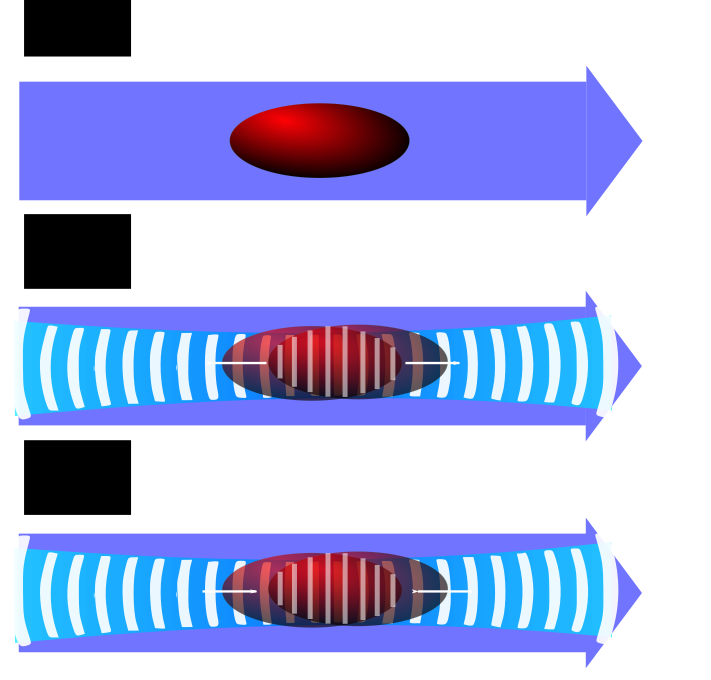
\includegraphics[width=1\columnwidth]{./Figures/KapitzaDirac.pdf}
\caption{In (A) the initial configuration is a ${}^{7}$Li BEC in a harmonic trap illuminated by a laser. (B) The trap is then dropped and the BEC is pulsed with a standing beam which scatters a fraction of the atoms into $\pm 2\hbar n_r k$ states.  (C) After a delay of $1$ ms, a second standing pulse will scatter another group out of the ground group which interfere with the first scattered group.} 
\label{fig:kapitz}
\end{figure}
%*********************************************************

The dipole potential created by a standing wave pulse is given by
\begin{equation}
\mathrm{U(\mathbf{x},t)=\frac{\hbar \Omega_R^2}{\Delta}f^2(t)\sin{(n_rk\mathbf{x})}}
\end{equation}
Where $\Omega_R$ is the Rabi frequency and $\Delta$ is the detuning away from the atomic transition frequency.  Here we have assumed $\Delta^2 \gg \Gamma/4$, where $\Gamma$ is the spontaneous decay rate. The function $f$ can be any function, but here we assume it is a simple step function resulting in a square wave pulse.
In the Raman-Nath approximation, the wave function immediately following a Kapitza-Dirac pulse is \cite{meystre,ketterle}
\begin{equation}
\left|\psi\right>=\left|\psi_0\right>e^{\frac{-i}{\hbar}\int dt'\,U(x,t')}=\left|\psi_0\right>e^{\frac{-i}{2\Delta}\Omega_R^2\tau}e^{\frac{i}{2\Delta}\Omega_R^2\tau\cos{(2n_rkx)}}
\end{equation}
Here we have defined $\tau=\int dt' f^2(t')$ which for a square wave pulse is simply the interaction time $\tau=t_{\mathrm{int}}$.  Note that for Kapitza-Dirac standing wave pulses we are assuming short interaction times relative to the recoil frequency (i.e.\, $t\ll 1/\omega_{\mathrm{rec}}$).  During the pulse we assume the atomic motion is negligible.   Making use of the identity 
\begin{equation}
e^{iA\cos{(B)}}=\sum\limits_{m=-\infty}^{\infty}i^mJ_m(A)e^{imB}
\end{equation}
we rewrite the wave function in terms of Bessel functions of the first kind
\begin{eqnarray}
\left|\psi\right>&=&\left|\psi_0\right>e^{\frac{-i\Omega_R^2\tau}{2\Delta}}\sum\limits_{m=-\infty}^{\infty}i^mJ_m\left(\frac{\Omega_R^2\tau}{2\Delta}\right)e^{i2mn_rkx} \nonumber \\
&=&e^{\frac{-i\Omega_R^2\tau}{2\Delta}}\sum\limits_{m=-\infty}^{\infty}i^mJ_m\left(\frac{\Omega_R^2\tau}{2\Delta}\right)\left|2mn_r\hbar k\right>
\end{eqnarray}
The Hamiltonian after the first pulse has acted is given by
\begin{eqnarray}
\hat{H}&=&\mathrm{\frac{\left(\hat{P}+\mathbf{d}\times\mathbf{B}\right)^2}{2m}-\frac{1}{2}\alpha E^2}\nonumber \\
&=&\mathrm{\frac{\hat{P}^2+2\mathbf{d}\times\mathbf{B}\hat{P}+\left(\mathbf{d}\times\mathbf{B}\right)^2}{2m}-\frac{1}{2}\alpha E^2}\nonumber \\
\end{eqnarray}

This is true since the R\"{o}ntgen term $\mathbf{d}\times\mathbf{B}$ is constant in this setup.  Since plane waves are eigenstates of the Hamiltonian, the eigenvalue of the term $\mathrm{\hat{P}}$ is
\begin{equation}
\mathrm{\hat{P} e^{\pm i2n_rkx}=\pm2n_r\hbar k e^{\pm i2n_rkx}}
\end{equation}
and therefore
\begin{equation}
\mathrm{\hat{H} e^{\pm i2n_rkx}=\left[\frac{\left(\pm 2n_r\hbar k+\mathbf{d}\times\mathbf{B}\right)^2}{2m}-\frac{1}{2}\alpha E^2\right]e^{\pm i2n_rkx}}
\end{equation}
We will drop the phase factor appearing in front of the summation in what follows. From here we can determine the state of the wave function $\psi$ at any time $t$ after the pulse.  In the position space representation this is found to be 
\begin{eqnarray}
&&\mathrm{\psi(x,t+\tau)=e^{\frac{-i\hat{H}t}{\hbar}}\psi(0)} \nonumber \\
&&=\mathrm{J_0\left(\frac{\Omega_R^2\tau}{2\Delta}\right)e^{\frac{-i}{\hbar}\left[\frac{\left(\mathbf{d}\times\mathbf{B}\right)^2}{2m}-\frac{1}{2}\alpha E^2\right]t}\left|0n_r\hbar k\right>} \nonumber \\
&+&\mathrm{iJ_1\left(\frac{\Omega_R^2\tau}{2\Delta}\right)\left(e^{i2n_rkx-\frac{it}{\hbar}\left[\frac{\left( 2n_r\hbar k+\mathbf{d}\times\mathbf{B}\right)^2}{2m}-\frac{1}{2}\alpha E^2\right]}\right)\left|2n_r\hbar k\right>} \nonumber \\
&+&\mathrm{iJ_1\left(\frac{\Omega_R^2\tau}{2\Delta}\right)\left(e^{-i2n_rkx-\frac{it}{\hbar}\left[\frac{\left(-2n_r\hbar k+\mathbf{d}\times\mathbf{B}\right)^2}{2m}-\frac{1}{2}\alpha E^2\right]}\right)\left|-2n_r\hbar k\right>} \nonumber \\
&&=\mathrm{e^{\frac{-it}{\hbar}\left(\frac{\left(\mathbf{d}\times\mathbf{B}\right)^2}{2m}-\frac{1}{2}\alpha E^2\right)}\bigg(J_0\left(\frac{\Omega_R^2\tau}{2\Delta}\right)\left|0n_r\hbar k\right>}\nonumber \\
&&+\mathrm{iJ_1\left(\frac{\Omega_R^2\tau}{2\Delta}\right)e^{i\left(2n_rkx-\frac{4\hbar^2n_r^2k^2t}{2m\hbar}-2n_rk\frac{\mathbf{d}\times\mathbf{B}}{m}t\right)}\left|2n_r\hbar k\right>}\nonumber \\
&&+\mathrm{iJ_1\left(\frac{\Omega_R^2\tau}{2\Delta}\right)e^{i\left(-2n_rkx-\frac{4\hbar^2n_r^2k^2t}{2m\hbar}+2n_rk\frac{\mathbf{d}\times\mathbf{B}}{m}t\right)}\left|-2n_r\hbar k\right>\bigg)}
\end{eqnarray}
Here we have made use of the identity $J_{-m}(\theta)=(-1)^mJ_{m}(\theta)$.  


We next apply another standing wave pulse to this wave function. We are interested in finding the probability of finding the atoms in the ground state $\left|0n_r\hbar k\right>$ after this second pulse, so we are only interested in the $\left|0n_r\hbar k\right>$ terms.
\begin{eqnarray}
&&\mathrm{\psi(x,t+2\tau)=\mathrm{e^{\frac{-it}{\hbar}\left(\frac{\left(\mathbf{d}\times\mathbf{B}\right)^2}{2m}-\frac{1}{2}\alpha E^2\right)}\bigg(J_0^2\left(\frac{\Omega_R^2\tau}{2\Delta}\right)\left|0n_r\hbar k\right>}}\nonumber \\
&&-\mathrm{J_1^2\left(\frac{\Omega_R^2\tau}{2\Delta}\right)e^{i\left(2n_rkx-\frac{4\hbar^2n_r^2k^2t}{2m\hbar}-2n_rk\frac{\mathbf{d}\times\mathbf{B}}{m}t\right)}\left|0n_r\hbar k\right>}\nonumber \\
&&-\mathrm{J_1^2\left(\frac{\Omega_R^2\tau}{2\Delta}\right)e^{i\left(-2n_rkx-\frac{4\hbar^2n_r^2k^2t}{2m\hbar}+2n_rk\frac{\mathbf{d}\times\mathbf{B}}{m}t\right)}\left|0n_r\hbar k\right>\bigg)}
\end{eqnarray}

The probability $p_0$ of finding the atoms in the ground state $\left|0n_r\hbar k\right>$ is

\begin{eqnarray}
\mathrm{p_0=|\left<\psi(x,t+2\tau)|0n_r\hbar k\right>|^2=J_0^4\left(\frac{\Omega_R^2\tau}{2\Delta}\right)}\nonumber \\
\mathrm{-4J_0^2\left(\frac{\Omega_R^2\tau}{2\Delta}\right)J_1^2\left(\frac{\Omega_R^2\tau}{2\Delta}\right)\cos{\left(\frac{4\hbar^2n_r^2k^2t}{2m\hbar}\right)}}\nonumber \\
\mathrm{\times cos{\left(2n_rkx-2\frac{\mathbf{d}\times\mathbf{B}}{m}n_rkt\right)}} \nonumber \\
\mathrm{+4J_1^4\left(\frac{\Omega_R^2\tau}{2\Delta}\right)\cos^2{\left(2n_rkx-2\frac{\mathbf{d}\times\mathbf{B}}{m}n_rkt\right)}}
\label{prob1}
\end{eqnarray}
The third term can be dropped as $J_0^2J_1^2\gg J_1^4$.  

Thus far we have neglected the impact that the doppler shifted dipole term would have on our ability to see the HMW phase.  Without the doppler shift, the dipole term $\frac{1}{2}\alpha E^2$ does not affect the probability since it contributes equally to all momentum states.  The doppler shift presents itself through the detuning 
\begin{equation}
\mathrm{\Delta_{\pm}=\Delta\left(1\pm \frac{\omega_{L}}{\Delta}\frac{v}{c}\right)}
\end{equation}
The doppler shifted dipole term is
\begin{equation}
\mathrm{\frac{1}{2}\alpha\left(1\mp \frac{\omega_{L}}{\Delta}\frac{v}{c}\right)E^2}
\end{equation}
If we include this term, the probability amplitude becomes
\begin{eqnarray}
&&\mathrm{p_0=|\left<\psi(x,t+2\tau)|0n_r\hbar k\right>|^2=J_0^4}\nonumber \\
&&\mathrm{-4J_0^2J_1^2\cos{\left(\frac{4\hbar^2n_r^2k^2t}{2m\hbar}\right)}\cos{\left(2n_rkx-2\frac{\mathbf{d}\times\mathbf{B}}{m}n_rkt+\frac{1}{2}\alpha E^2\frac{\omega_L}{\hbar \Delta}\frac{v}{c}t\right)}} \nonumber \\
&&\mathrm{+4J_1^4\cos^2{\left(2n_rkx-2\frac{\mathbf{d}\times\mathbf{B}}{m}n_rkt+\frac{1}{2}\alpha E^2\frac{\omega_L}{\hbar \Delta}\frac{v}{c}t\right)}} \nonumber \\
&&=J_0^4-\mathrm{-4J_0^2J_1^2\cos{\left(\frac{4\hbar^2n_r^2k^2t}{2m\hbar}\right)}\cos{\left(2n_rkx-2\alpha E^2\frac{n_rkt}{mc}\left(1-\frac{\omega_L}{2\Delta}\right)\right)}} \nonumber \\
\label{prob2}
\end{eqnarray}

Where in the last line we have dropped the higher order term. Comparing  Eq.\ (\ref{prob1}) with  Eq.\ (\ref{prob2}) we see that the dipole effect must be dealt with by running the traveling wave laser in both directions in order to isolate the contribution from the HMW phase.
\vspace{5mm}
 
The HMW phase is incredibly small and requires a large laser intensity to become visible.  We can get a sense of the required magnitude of the HMW to obtain an observable effect by considering the time-frequency uncertainty relation $\Delta \nu \Delta t>1$.  This uncertainty relation tells us that during a 1ms sampling time, we require a frequency shift of $\Delta \nu>$ 1kHz. Setting this equal to the HMW frequency $2\frac{\mathbf{d}\times\mathbf{B}}{m}n_rkt$ we find that $\alpha I>2.3\times 10^{-25}$. Here $I$ is the intensity and $\alpha$ is the polarizability. If we use $\alpha=4\times10^{-36}\,\mathrm{F\cdot m^2}$ as we did in the previous section, then we require a laser intensity of $\mathrm{I=6 \times 10^{6}\,W/cm^2}$. 

Spontaneous emission is a major concern as it affects the visibility of the interference fringes required to observe the HMW effect.  If the separation distance $d$ between the out-coupled sample of atoms in the state $\ket{2\hbar n_r k}$ and the ground atoms $\ket{0\hbar n_r k}$ is larger than the wavelength of the probe laser interacting with the sample, then any spontaneous emission would destroy the coherence of the experiment.  The follows from the fact that under such circumstances, a spontaneous event would allow an observer to positively identify the sample from which the photon was emitted.  This would then break the superposition state of the two samples, thus eliminating the ability to interfere the two states.  
This however is not the case here.  Let us take the dimensions of the condensate to be 300 $\mu$m $\times$ 20 $\mu$m \cite{BEC}. The recoil velocity of Lithium is approximately $\mathbf{v}_{\mathrm{rec}}=9$ cm/s.  Therefore, during the 1 ms that the two samples are separating, the total separation distance is $d=1.8\times 10^{-4}$ m. Therefore the majority of the condensate overlaps throughout the process. Pritchard's group \cite{decoherence} has measured the effects of spontaneous emission on decoherence and has found that for such small separation distances the fringe contrast will not be overly diminished. 

 In free space, such a intensity output would be difficult to achieve, but by placing the atom in a ring cavity (Figure \ref{fig:ringcavity}) we can enhance the intensity by a factor of $2\mathcal{F}/\pi$ \cite{spectroscopy}, where $\mathcal{F}$ is the finesse of the cavity system.  The cavity finesse required will of course depend on the intensity of the pump laser.
A caveat of placing the atom in a cavity system is that a back action of the atom on the intra-cavity field can alter the cavity modes. Collective atom recoil lasing (CARL) instabilities can arise in such a system \cite{courteille}.  CARL labels any type of behavior in a atom-cavity system in which feedback from the atom on the cavity modes cause atomic density modulation and/or growth of optical fields.  As an example of a potential pitfall to placing the atom inside a cavity is the possibility that the atom will radiate into the oppositely traveling mode of the ring cavity and hence setup a lattice.  Such an effect would obviously be undesirable as the dipole force generated by an optical lattice would add an extra layer of complication to disentangling the HMW phase from other effects.  For a single atom massively detuned from the cavity mode, it turns out that even for such high intensities such as those required to see the HMW phase, the CARL threshold is not reached \cite{hemmerich} and the back action effects may safely be ignored.  
%***************************figure**********************
\begin{figure}[htp]
\includegraphics[width=1\columnwidth]{./Figures/RingCavity.pdf}
\caption{A schematic for the high finesse ring cavity setup used to enhance the intensity of the traveling wave. The cavity mode must be massively detuned from the atomic transition in order to suppress spontaneous emission $\gamma$. } 
\label{fig:ringcavity}
\end{figure}
%*********************************************************

Using a Kaptiza-Dirac pulse of wavelength $\lambda=671\,\mathrm{nm}$ the value of the recoil frequency term is $n_r\hbar kx =3.4\times 10^3$, while $\frac{4\hbar^2n_r^2k^2t}{2m\hbar}$ is approximately twice the size of the recoil term. The R\"{o}ntgen term which is responsible for the HMW phase is  $2\frac{\mathbf{d}\times\mathbf{B}}{m}n_rk\,t=9.5\,t$/s.  
In figure \ref{fig:ft2hk} we plot the probability of finding the atom in the ground state (Eq.\ (\ref{prob1})) with and without the HMW phase using these values. The red line shows the probability to find the atoms in the ground state without the HMW phase, while the solid blue lines include the HMW phase. In \ref{fig:ft2hk} we plot the Fourier transform.  
%***************************figure**********************
\begin{figure}[htp]
\includegraphics[width=1\columnwidth]{./Figures/Probability2hknew.pdf}
\caption{A plot of the probability of finding the atoms in the ground state $\mathrm{p_0=|\left<\psi(x,t+2\tau)|0n\hbar k\right>|^2}$. The red line show the probability of finding the atoms in the ground state without the HMW phase, while the blue line include the HMW phase. The intensity of the laser is $I_1=9.7\times 10^6\, \mathrm{W/cm^2}$.} 
\label{fig:prob}
\end{figure}
%*********************************************************
%***************************figure**********************
\begin{figure}[htp]
\includegraphics[width=1\columnwidth]{./Figures/FT2hk.pdf}
\caption{The time-discrete fourier transform of Eq.\ (\ref{prob1}) using 1 ms of sampling with a 1 $\mu$s sample rate. The dotted blue line shows the fourier transform without the HMW phase, while the red line include the HMW phase. The effect of the HMW on the Fourier transform is most apparent in the magnitude change, while the frequency shift is difficult to see. It is important to note that we chose parameters in which the difference is just beginning to emerge.} 
\label{fig:ft2hk}
\end{figure}
%*********************************************************


A possible enhancing technique which may also be implemented to increase the size of the R\"{o}ntgen term is to consider large momentum transfer beamsplitters (LMT). Thus far we have only considered recoil momentum kicks of the form $2n_r\hbar k$. However, it is possible to use large momentum transfers on the order of $10 n_r\hbar k-100 n_r\hbar k$ \cite{kasevich}.  Using such an LMT, we would could significantly increase the effects of the HMW phase.  This however also works against us by increasing the separation distance between samples, and hence decreasing the fringe visibility.  A better option is to simply increase the intensity slightly at the cost of a modest decrease in visibility due to spontaneous emission.  In Figures \ref{fig:prob10} and \ref{fig:ft10hk} we plot Eq.\ (\ref{prob1}) and the time-discrete Fourier transform using an intensity of $I_2=9.7\times 10^7\, \mathrm{W/cm^2}$.

%***************************figure**********************
\begin{figure}[htp]
\includegraphics[width=1\columnwidth]{./Figures/Probability10hknew.pdf}
\caption{A plot of the probability of finding the atoms in the ground state $\mathrm{p_0=|\left<\psi(x,t+2\tau)|0n\hbar k\right>|^2}$. The red line show the probability of finding the atoms in the ground state without the HMW phase, while the blue line include the HMW phase. Here the difference between the two is more apparent. The intensity of the laser is set to $I_1=9.7\times 10^7\, \mathrm{W/cm^2}$.} 
\label{fig:prob10}
\end{figure}
%*********************************************************
%***************************figure**********************
\begin{figure}[htp]
\includegraphics[width=1\columnwidth]{./Figures/FT10hk.pdf}
\caption{The time-discrete fourier transform of Eq.\ (\ref{prob1}) using an increased intensity $I_1=9.7\times 10^7\, \mathrm{W/cm^2}$.  The separation between the peaks is much more striking here.} 
\label{fig:ft10hk}
\end{figure}

%*********************************************************




%==============================
\newpage
\section{Laguerre Beams}
The setup we consider is a trapped BEC in an optical ring trap as outlined in \cite{phillips, boshier}.  The BEC is then irradiated with a single Laguerre-Gaussian (LG) beam. Note that this is different from typical setups \cite{campbell} in which the Laguerre-Gauss beam is accompanied by a counter-propagating Gaussian beam.  The interaction of the two beams creates a standing wave profile, producing a dipole force on the BEC which is responsible for the transfer of angular momentum. What we wish to show is that the HMW phase can be observed from a setup in which only a single LG beam is present. Consider an LG mode $L_0^l$, linearly polarized in the transverse x-direction as shown in figure \ref{fig:setup}.  The magnitude of the Laguerre-Gauss mode $u_0^l$ at $z=0$ can be written in cylindrical coordinates as \cite{Willke}
\begin{equation} 
\mathrm{u_0^l(\bold{r,\phi})=A_0 \sqrt{\frac{2}{\pi w_0^2}}\sqrt{\frac{1}{l!}}\exp{\frac{-2r^2}{w^2}}\left(\frac{\sqrt{2}r}{w}\right)^{l}\exp{il\phi}}
\label{LGmode}
\end{equation}
%***************************figure**********************
\begin{figure}[htp]
\includegraphics[width=1\columnwidth]{./Figures/azimuthal.pdf}
\caption{A Laguerre-Gauss field with linear polarization acts on an atomic circuit trap. The wavefronts of the beam have an azimuthal component giving the Poynting vector a non-zero angular term.  This acts on the atom circuit to generate an azimuthal flow.} 
\label{fig:setup}
\end{figure}
%*********************************************************
where $A_0$ is the amplitude, and $w_0$ is the beam waist. The vector potential $\mathrm{A(\bold{r,\phi,z})}$ associated with such a mode can be written as
\begin{equation} 
\mathrm{A(\bold{r,\phi,z})}=\mathrm{u_0^l(\bold{r,\phi})\exp{i(\bold{kz}-\omega t)}\hat{\bold{x}}}
\label{vpotential}
\end{equation}
The electric and magnetic fields may then be obtained via
\begin{eqnarray}
&&\mathrm{E(\bold{r,\phi,z})= i\omega \left(A(\bold{r,\phi,z})+\frac{\nabla\left(\nabla\cdot A(\bold{r,\phi,z})\right)}{k^2}\right)} \nonumber \\
&&\mathrm{B(\bold{r,\phi,z})=\nabla\times A(\bold{r,\phi,z})}
\end{eqnarray}
We apply the paraxial approximation in which we neglect terms which have derivatives in the longitudinal direction (z-direction) along with higher derivatives of the transverse components
\begin{eqnarray}
&&\mathrm{E(\bold{r,\phi,z})= i\omega u(\bold{r,\phi})\exp{i(\bold{kz}-\omega t)}\hat{\bold{x}} -c \frac{\partial u(\bold{r,\phi})}{\partial x}\exp{i(\bold{kz}-\omega t)}\hat{\bold{z}}} \nonumber \\
&&\mathrm{B(\bold{r,\phi,z})=ik u(\bold{r,\phi})\exp{i(\bold{kz}-\omega t)}\hat{\bold{y}}-\frac{\partial u(\bold{r,\phi})}{\partial x}\exp{i(\bold{kz}-\omega t)}\hat{\bold{z}}} \nonumber \\
\end{eqnarray}
We first wish to find the azimuthal component of $\mathcal{\alpha E\times B}$.  
\begin{equation}
\mathrm{\left(\alpha E\times B\right)_{\phi}=\frac{4A_0^2 \alpha ck 2^l}{w_0^{2l+2} \pi l!}r^{2l}\exp{\frac{-2r^2}{w^2}}\left[\frac{2}{w_0^2}-lr^{-2}\right]}
\end{equation}
This term is the only component responsible for giving us an HMW phase around a circuit.  However, since we also wish to write the LG mode in terms of the output power of the laser $P$, we also want the z-component of $E\times B$ in order to find the intensity of the laser.  
\begin{equation}
\mathrm{\left(\alpha E\times B\right)_{z}=\frac{c^2 k^2 A_0^2 2^l}{w_0^{2l+2} \pi l!}r^{2l}\exp{\frac{-2r^2}{w^2}}}
\end{equation}
The intensity of a beam is given by $\mathrm{I=\frac{1}{2}\epsilon_0 c^2 \left(\alpha E\times B\right)_{z}}$ which can be rewritten as $\mathrm{I=\frac{1}{2}\epsilon_0 c^2 k^2 A_0^2 |u_0^l|^2}$ in terms of the LG modes.  Integrating this over the area gives the power $\mathrm{P=\frac{1}{2}\epsilon_0 c^2 k^2 A_0^2}$ which is simple as the LG modes are normalized.  This yields $\mathrm{A_0=\sqrt{\frac{2P}{\epsilon_0 c^2 k^2}}}$
From here we can work out the HWM phase by making use of the curl theorem $\mathcal{\int\!\left(\nabla \times \bold{A}\right)\cdot\! d\bold{a}=\oint \!\bold{A}\cdot \!d\bold{l}}$ 
\label{HMW}
\begin{equation}
\mathrm{\exp{iS/\hbar}=i\frac{16P \alpha ck 2^l}{\hbar w_0^{2l+2} \epsilon_0 ck l!}\int_0^a\!\exp{\frac{-2r^2}{w^2}}\left[ \frac{2}{w_0^2}r^{2l+1}-lr^{2l-1}\right]\!dr}
\end{equation}
where $\mathrm{a}$ is the radius of the atom circuit produced by the trap.  This integral can be solved analytically 
\begin{equation}
\mathrm{\int_0^a\!\exp{\frac{-2r^2}{w^2}}\left[ \frac{2}{w_0^2}r^{2l+1}-lr^{2l-1}\right]\!dr = -\frac{1}{2}\exp{\frac{-2a^2}{w^2}}a^{2l}}
\end{equation}
The maximum value for which occurs at a radius of $\mathrm{a=w_0/sqrt{2}}$.  Plugging this into Eq.\ (\ref{HMW}) gives a maximum phase of
\begin{equation}
\mathrm{\exp{iS/\hbar}=exp{\left(-i\frac{8P \alpha 2^l}{\hbar e^1 w_0^{2} \epsilon_0 ck l!}\right)}}
\end{equation}
Recently Willke's \cite{Willke} group was able to generate high order ($u^3_3$) Laguerre-Gauss beams with high laser power (83 Watt). Using $\alpha=9.6\times10^{-35}{\mathrm{cm}}^2\mathrm{V}$ along with the parameters used by Willke's group we find the HMW phase shift to be approximately $-4\times10^5$ radians. 
We begin with the Hamiltonian for a BEC in an elliptical trap interacting
with a Laguerre-Gauss beam.
\[
i\hbar\partial_{t}\psi=H\psi=\left[-\frac{\hbar^{2}}{2m}\left(\frac{1}{R}\frac{\partial}{\partial\theta}+\frac{i}{\hbar}\vec{d}\times\vec{B}\right)^{2}-V_{0}\cos\theta\right]\psi
\]
The potential amplitude $V_{0}$ can be adjusted as needed. The Poynting
term $\vec{d}\times\vec{B}$ is given by:
\[
\vec{d}\times\vec{B}=\frac{-4\alpha P}{c^{2}\epsilon_{0}k\pi w_{0}^{4}}re^{-2r^{2}/w_{0}^{2}}\equiv C_{1}re^{-2r^{2}/w_{0}^{2}}
\]
where$w_{0}$is the gaussian beam width, $r$ is the radius, $P$
is the power of the beam, and$\alpha$ is the atomic polarizibility.
We are now ready to expand out the Hamiltonian and see what we get.
Let $\psi=e^{in\theta}/\sqrt{2\pi R}$

\[
H\psi=\left[-\frac{\hbar^{2}}{2m}\left(\frac{1}{R}\frac{\partial}{\partial\theta}+\frac{i}{\hbar}\vec{d}\times\vec{B}\right)^{2}-V_{0}\cos\theta\right]\psi
\]


\[
=\left[-\frac{\hbar^{2}}{2m}\left(-\left(\frac{n}{R}\right)^{2}-2\frac{1}{\hbar}\vec{d}\times\vec{B}\left(\frac{n}{R}\right)-\left(\frac{\vec{d}\times\vec{B}}{\hbar}\right)^{2}\right)-V_{0}\cos\theta\right]\frac{e^{in\theta}}{\sqrt{2\pi R}}
\]


\[
=\left[\frac{\hbar^{2}}{2m}\left(\frac{n}{R}+\frac{\vec{d}\times\vec{B}}{\hbar}\right)^{2}-V_{0}\cos\theta\right]\frac{e^{in\theta}}{\sqrt{2\pi R}}
\]
Now what this tells us is that in order to go from the $n=0$ parabola
to the $n=1$ we require $\frac{\vec{d}\times\vec{B}}{\hbar}=\frac{1}{r}$.
This tells us the laser power we need to input in order to get any
rotation. Note this has nothing to do with the speed at which we are
sweeping, we simply want to know how much power we will need to see
any rotation. Our requirment for the Poynting vector to be strong
enough to generate a vortex is given by

\[
\frac{4\alpha P}{\hbar c^{2}\epsilon_{0}k\pi w_{0}^{4}}re^{-2r^{2}/w_{0}^{2}}=\frac{1}{r}
\]
where $P$ is the power, and $w_{0}$ is the beam waist length. We
also make use Duncan's equations for the dynamic polarizibility $\alpha$

\[
\alpha\left(\omega_{L}\right)=\frac{1}{\hbar}\left(\frac{\mu_{A}^{2}}{\Delta+2\pi\times267\times10^{6}}+\frac{\mu_{B}^{2}}{\Delta}\right)
\]
where $\mu_{A}\approx\mu_{B}\approx1.45\times10^{-29}$Cm, and $\Delta$
is the detuning. The spontaneous emission scattering rate $\Gamma_{sc}$
is given by

\[
\Gamma_{sc}=\frac{3\pi c^{2}}{2\hbar\omega_{0}^{3}}\left(\frac{\Gamma}{\Delta}\right)^{2}I=\frac{6c^{2}\Gamma^{2}P}{\sqrt{2}\hbar\omega_{0}^{3}w_{0}^{3}k\Delta^{2}}
\]
Where $\omega_{0}=2\pi\times3.84\times10^{14}s^{-1}$ is the D2-line
transition frequency, $\Gamma=3.61\times10^{7}s^{-1}$ is the natural
line width. Here we used the intensity $I$ at $r=w_{0}/\sqrt{2}$
given by

\[
I=\frac{1}{2\mu_{0}}E\times B=\frac{4P}{\pi w_{0}^{4}k}re^{-2r^{2}/w_{0}^{2}}=\frac{4P}{\sqrt{2}\pi w_{0}^{3}k}
\]
Rearranging the scattering rate equation and solving for the power
$P$ yields

\[
P=\frac{\sqrt{2}\hbar\omega_{0}^{3}w_{0}^{3}k\Delta^{2}\Gamma_{sc}}{6c^{2}\Gamma^{2}}
\]
We can then plug this into the equation
\[
\frac{4\alpha P}{\hbar c^{2}\epsilon_{0}k\pi w_{0}^{4}}re^{-2r^{2}/w_{0}^{2}}=\frac{1}{r}
\]
\[
\Rightarrow\frac{\sqrt{2}\omega_{0}^{3}w_{0}\alpha\Delta^{2}\Gamma_{sc}}{3c^{4}\epsilon_{0}\pi\Gamma^{2}}=1
\]
This now gives us a relationship between the different parameters
involved. Our job is to find a sweet spot in which the scattering
rate is managable. We now substitute in the formula for the dynamic
polarizibility $\alpha$ in the limit where detuning dominates. In
this limit we have

\[
\alpha\left(\omega_{L}\right)\approx\frac{2}{\hbar}\frac{\mu_{B}^{2}}{\Delta}
\]
and obtain
\[
\frac{2\sqrt{2}\omega_{0}^{3}w_{0}\mu_{B}^{2}\Delta\Gamma_{sc}}{3\hbar c^{4}\epsilon_{0}\pi\Gamma^{2}}=1
\]
Solving this for the scaterring rate $\Gamma_{sc}$

\[
\Gamma_{sc}=\frac{3\hbar c^{4}\epsilon_{0}\pi\Gamma^{2}}{2\sqrt{2}\omega_{0}^{3}w_{0}\mu_{B}^{2}\Delta}
\]
Let's now assume we are using a $CO_{2}$ with a wavelength of $10\times10^{-6}$m,
and frequency $3\times10^{13}$. This would give us a massive detuning
of $\Delta\thickapprox\omega_{0}$. Plugging in the values of the
other parameters which are found above, gives us

\[
\Gamma_{sc}=\frac{4.4}{w_{0}}
\]
We can see that the scattering rate is actually quite small, as long
as we keep the radius of the trap large. Let the radius be $r=5\times10^{-6}$,
then the scattering rate is approximately $10^{6}$. This gives us
a time frame of about $10^{-6}$s. The power $P$ needs to be quite
large as a result

\[
P=\frac{\hbar c^{2}\epsilon_{0}k\pi w_{0}^{2}}{2\alpha}=5.5\times10^{5}
\]
The Landau-Zener formula which states that the probability of making
a diabatic transition is given by

\[
P=e^{-2\pi\Theta}
\]


\[
\Theta=\frac{d^{2}/\hbar}{\frac{d}{dt}\left(E_{1}-E_{0}\right)}
\]
where $d$ is the off diagona\textbackslash{}frac\{4\textbackslash{}alpha
P\}\{\textbackslash{}hbar c\textasciicircum{}\{2\}\textbackslash{}epsilon\_\{0\}k\textbackslash{}pi
w\_\{0\}\textasciicircum{}\{4\}\}re\textasciicircum{}\{-2r\textasciicircum{}\{2\}/w\_\{0\}\textasciicircum{}\{2\}\}l
element in the Hamiltonian. For our system, this term corresponds
to $V_{0}/2$. We can find the energy difference easily enough.

\[
E_{0}=\frac{\hbar^{2}}{2m}\left(\frac{\vec{d}\times\vec{B}}{\hbar}\right)^{2}-V_{0}
\]


\[
E_{1}=-\frac{\hbar^{2}}{2m}\left(-\left(\frac{1}{r}\right)^{2}-2\frac{1}{\hbar}\vec{d}\times\vec{B}\left(\frac{1}{r}\right)-\left(\frac{\vec{d}\times\vec{B}}{\hbar}\right)^{2}\right)-V_{0}
\]
Then we get
\[
\frac{d}{dt}\left(E_{1}-E_{0}\right)=2\frac{\hbar}{mr}\frac{d}{dt}\left(\vec{d}\times\vec{B}\right)
\]
We next need to determine how fast we need to sweep at to go from
one parabola to the other in the allotted time (i.e before spontaneous
emission burns us). Well the time doesn't seem to be a problem so
let's sweep from $\vec{d}\times\vec{B}=0$ to the necessary $\vec{d}\times\vec{B}=\hbar/r$
intensity linearly in 1s. Plugging this into the Landau-Zener equation
we get

\[
\Theta=\frac{V_{0}^{2}/4\hbar}{2\frac{\hbar^{2}}{mr^{2}}}=\frac{V_{0}^{2}mr^{2}}{8\hbar^{3}}
\]
Now if $V_{0}$ is the potential due to gravity
\[
V_{0}=-G\frac{M_{E}m}{r}=-1.0\times10^{-17}N/m
\]
Using this value, even though it's small we'll still get perfectly
adiabatic following.





%==============================
\section{Summary and Conclusions}

yup

%================================================================

%================================================================
\chapter{Quantum Representations}
\chaptermark{QR}
%================================================================



\section{Introduction}
\label{sec:intro}

In this section, we show that while both forms of the electromagnetic momentum density are correct, they speak to different representations of the Hamiltonian. They are linked to two different representations of the direct coupling Hamiltonian which we show to be tied intimately with the Aharonov-Casher and the He-McKellar-Wilkens geometric phase.  The phases naturally arise as a result of enforcing invariance in the equations of motion.
The Abraham and Minkowski representations are shown to be related through a unitary transformation which gives rise to both the HMW and the AC phase. 

\section{The Abraham/Minkowski representation}
\label{sec:DC}

We begin with the direct coupling Lagrangian for a polarizable/magnetizable atom interacting with an electromagnetic field \cite{thirunamachandran}
\begin{eqnarray}
L&=&\frac{1}{2}mv^2+\frac{\epsilon_0}{2}\int\left(\dot{A}^2-c^2\left(\nabla\times \mathbf{A}\right)^2\right)\,d^3\mathbf{r} \nonumber \\
 &-&\int\left(\mathbf{P}\cdot\dot{\mathbf{A}}\right)\,d^3\mathbf{r}+\int\left( \left[\nabla\times\mathbf{M}\right]\cdot\mathbf{A}\right)\,d^3\mathbf{r}
\end{eqnarray}
Where $\mathbf{A}$ is the vector potential, $\mathbf{P}$ is the polarization , and $\mathbf{M}$ is the magnetization.  
Grouping terms we get
\begin{eqnarray}
L&=&\frac{1}{2}mv^2+\frac{1}{2}\int\left(-\dot{\mathbf{A}}\cdot\left(-\epsilon_0\dot{\mathbf{A}}+\mathbf{P}\right)\right)\,d^3\mathbf{r} \nonumber \\
&-&\int\left( \left(\nabla\times \mathbf{A}\right)\cdot\left(\frac{1}{\mu_0}\nabla\times \mathbf{A}-\mathbf{M}\right)\right)\,d^3\mathbf{r} 
\end{eqnarray}
Using the definitions for the electric and magnetic fields
\begin{eqnarray}
\mathbf{E}&=&-\frac{\partial \mathbf{A}}{\partial t} \\
\mathbf{B}&=&\nabla\times\mathbf{A}
\end{eqnarray}
along with the auxiliary field definitions
\begin{eqnarray}
\mathbf{D}&=&\epsilon_0\mathbf{E}+\mathbf{d}\delta\left(\mathbf{r}-\mathbf{r}_{\mathrm{atom}}\right) \\
\mathbf{H}&=&\frac{1}{\mu_0}\mathbf{B}-\mathbf{m}\delta\left(\mathbf{r}-\mathbf{r}_{\mathrm{atom}}\right)
\end{eqnarray}
we arrive at a simplified representation given in terms of the electric and magnetic fields
\begin{eqnarray}
L&=&\frac{1}{2}mv^2 + \frac{1}{2}\int\left(\mathbf{D}\cdot\mathbf{E}-\mathbf{H}\cdot\mathbf{B}\right)\,d^3\mathbf{r} \nonumber \\
&=&\frac{1}{2}mv^2 + \frac{1}{2}\int\left(\epsilon E^2-\frac{1}{\mu}B^2\right)\,d^3\mathbf{r} 
\label{lagrangian1}
\end{eqnarray}

This is not the full Lagrangian yet. In the atom's reference frame the Lorentz transformed fields are $\bar{\mathbf{E}}=\mathbf{E}+\mathbf{v}\times\mathbf{B}$ and $\bar{\mathbf{B}}=\mathbf{B}-\epsilon_0\mu_0\left(\mathbf{v}\times\mathbf{E}\right)$ (to first order in v/c). The actual electric field that the atom interacts with is not the electric field as seen in the lab frame, but the Lorentz transformed field as seen in the atom's frame.  Hence, the true Lagrangian is
\begin{eqnarray}
&L&=\frac{1}{2}mv^2 + \frac{1}{2}\int\left(\mathbf{D}\cdot\mathbf{E}-\mathbf{H}\cdot\mathbf{B}\right)\,d^3\mathbf{r} \nonumber \\
&-& \int\mathbf{v}\cdot\left(\mathbf{D}\times\mathbf{B}\right)\,d^3\mathbf{r}
+ \int\mathbf{v}\cdot\frac{\mathbf{E}\times\mathbf{H}}{c^2}\,d^3\mathbf{r} + \mathrm{H.O.}
\label{lagrangian2}
\end{eqnarray}
The canonical momentum for the atom is then
\begin{eqnarray}
\mathbf{p}&=&m\mathbf{v}- \int\left(\mathbf{D}\times\mathbf{B}-\frac{\mathbf{E}\times\mathbf{H}}{c^2}\right)\,d^3\mathbf{r} \nonumber \\
&\equiv & m\mathbf{v}-\mathbf{d}\times\mathbf{B}-\frac{\mathbf{E}\times\mathbf{m}}{c^2}
\label{canonical}
\end{eqnarray}
Here $\mathbf{d}$ and  $\mathbf{m}$ are the electric and magnetic dipole moments respectively.  The corresponding Hamiltonian is then found to be
\begin{eqnarray}
H&=&\frac{1}{2m}\left(\mathbf{p}+ \mathbf{d}\times\mathbf{B}+\frac{\mathbf{E}\times\mathbf{m}}{c^2}\right)^2\nonumber \\
&+&\frac{1}{2}\int\left(\mathbf{D}\cdot\mathbf{E}+\mathbf{H}\cdot\mathbf{B}\right)\,d^3\mathbf{r}
\label{hamilton1}
\end{eqnarray}
The corresponding Schr\"{o}dinger equation for the Hamiltonian
\begin{eqnarray}
i\hbar\dot{\psi}&=&\frac{1}{2m}\left(\mathbf{p}+ \mathbf{d}\times\mathbf{B}+\frac{\mathbf{E}\times\mathbf{m}}{c^2}\right)^2\psi\nonumber \\
&+&\left(\frac{1}{2}\int\left(\mathbf{D}\cdot\mathbf{E}+\mathbf{H}\cdot\mathbf{B}\right)\,d^3\mathbf{r}\right)\,\psi \nonumber\\
\label{schrodinger1}
\end{eqnarray}
The last term in Eq.\ (\ref{schrodinger1}) may be rewritten by making use of Poynting's theorem  \cite{griffiths}
\begin{equation}
\mathbf{E}\cdot\mathbf{J}_{\mathrm{f}}=-\frac{1}{2}\frac{\partial}{\partial t}\left(\mathbf{D}\cdot\mathbf{E}+\mathbf{B}\cdot\mathbf{H}\right)-\nabla\cdot\left(\mathbf{E}\times\mathbf{H}\right)
\label{poynting1}
\end{equation}
Since there are no free currents, $\mathbf{J}_{\mathrm{f}}=0$.  This allows us to write
\begin{equation}
\frac{1}{2}\left(\mathbf{D}\cdot\mathbf{E}+\mathbf{B}\cdot\mathbf{H}\right)=-\int\nabla\cdot\left(\mathbf{E}\times\mathbf{H}\right)\,\,dt'
\label{poynting2}
\end{equation}
We can rewrite the second term in  Eq.\ (\ref{poynting2}) through a change in variable which leads to
\begin{eqnarray}
&&\nabla\rightarrow\frac{1}{c}\frac{\partial}{\partial t}\\
&&\int\,dt\rightarrow\frac{1}{c}\int\,d\mathbf{r}'
\end{eqnarray}
Thus Poynting's theorem allows us to write
\begin{equation}
\frac{1}{2}\left(\mathbf{D}\cdot\mathbf{E}+\mathbf{B}\cdot\mathbf{H}\right)=-\frac{\partial}{\partial t}\int\left(\frac{\mathbf{E}\times\mathbf{H}}{c^2}\right)\cdot\,dl
\label{poynting3}
\end{equation}
Substituting this into Eq.\ (\ref{schrodinger1}) gives
\begin{eqnarray}
i\hbar\dot{\psi}&=&\frac{1}{2m}\left(\mathbf{p}+ \mathbf{d}\times\mathbf{B}+\frac{\mathbf{E}\times\mathbf{m}}{c^2}\right)^2\psi\nonumber \\
&-&\left(\frac{\partial}{\partial t}\int \mathbf{S}_{\mathrm{Abr}}\cdot\,dl\right)\,\psi \nonumber\\
\label{schrodinger3}
\end{eqnarray}
This is what we will call the Abraham representation. The first term on the right is the kinetic momentum of the atom, while the second term is the energy due to the Abraham momentum 
\begin{equation}
\mathbf{S}_{\mathrm{Abr}}=\int\frac{\mathbf{E}\times\mathbf{H}}{c^2}\,d^3\mathbf{r}
\end{equation}
Both the AC and the HMW effect originate in this representation as dynamic phases through the kinetic momentum \cite{boyd}
\begin{equation}
m\mathbf{v}=m\frac{\partial H}{\partial \mathbf{p}}=m\left(\mathbf{p}+ \mathbf{d}\times\mathbf{B}+\frac{\mathbf{E}\times\mathbf{m}}{c^2}\right)
\end{equation}


 The Abraham representation is in no ways unique.  We can transform the Sch\"{o}dinger equation into the Minkowski representation through a unitary transformation by writing the wave function as
\begin{equation}
\mathrm{\psi=\Psi\exp{\left[-\frac{\mathrm{i}}{\mathrm{\hbar}}\int\mathbf{S}\cdot d\mathbf{l}\right]}}
\label{minkrep}
\end{equation}
Where $\mathbf{S}=\mathbf{d}\times\mathbf{B}+\epsilon_0\mu_0\mathbf{E}\times\mathbf{m}$. Substituting this back into Eq.\ (\ref{schrodinger3}) gives us
\begin{eqnarray}
&&i\hbar\dot{\Psi}\,\,\exp{\left[-\frac{i}{\hbar}\int\mathbf{S}\cdot d\mathbf{l}\right]} \nonumber \\
&+&\Psi\,\left(\frac{\partial}{\partial t}\int\mathbf{S}\cdot d\mathbf{l}\right)\,\exp{\left[-\frac{i}{\hbar}\int\mathbf{S}\cdot d\mathbf{l}\right]}\nonumber \\
&=&-\frac{\hbar^2\left(\nabla^2\Psi\right)}{2m}\,\exp{\left[-\frac{\mathrm{i}}{\hbar}\int\mathbf{S}\cdot d\mathbf{l}\right]} \nonumber\\
&-& \left(\frac{\partial}{\partial t}\int\frac{\mathbf{E}\times\mathbf{H}}{c^2}\cdot\,d\mathbf{l}\right)\,\Psi\,\exp{\left[-\frac{i}{\hbar}\int\mathbf{S}\cdot d\mathbf{l}\right]}
\label{schrodinger4}
\end{eqnarray}
Cancelling out the unitary term and rearranging gives
\begin{equation}
i\hbar\dot{\Psi}=\frac{\mathbf{p}^2}{2m}\Psi 
 -\left(\frac{\partial}{\partial t}\int \mathbf{S}_{\mathrm{Min}}\cdot d\mathbf{l}\right)\Psi 
\label{schrodinger5}
\end{equation}
Here the first term on the right is the canonical momentum of the atom, while the second term is now the energy due to the Minkowski momentum
\begin{equation}
\mathbf{S}_{\mathrm{Min}}=\int\left(\mathbf{D}\times\mathbf{B}\right)\,d^3\mathbf{r}
\end{equation}
  As both representations are equally valid, we have arrived at the well known relationship between the kinetic/canonical momentum of an atom and the Abraham/Minkowski momentum of the interacting electromagnetic field
\begin{equation}
m\mathbf{v}+\mathbf{S}_{\mathrm{Abr}}=\mathbf{p}+\mathbf{S}_{\mathrm{Min}}
\end{equation}

\vspace{5mm}

Suppose now we know the ground state wave function of the system beforehand $\psi_0$. From Eq.\ (\ref{minkrep}) we see if we decided to use the Minkowski formulation and naively plugged in $\Psi=\psi_0$, we would obtain an incorrect result.  Using the Minkowski representation forces us to use the initial wave function 
\begin{equation}
\Psi=\psi_0\exp{\left[-\frac{\mathrm{i}}{\mathrm{\hbar}}\int \left(\mathbf{d}\times\mathbf{B}+\frac{\mathbf{E}\times\mathbf{m}}{c^2}\right)\cdot d\mathbf{l}\right]}
\end{equation}
This is precisely the Aharonov-Casher and the He-McKellar Wilkens phase.  The AC and HMW effect appear in the Minkiowski representation as geometric phases, in contrast to the dynamic phase portrayal in the Abraham representation.   

\section{Conclusion}
\label{conclusion}

We began by showing how the classical Lagrangian for a polarizable/magnetizable atom interacting with an electromagnetic field must be modified by considering the Lorentz transformed interactions as seen from the atom's reference frame.  We were then able to show that the corresponding Hamiltonian yielded the Abraham momentum through Poynting's theorem. By transforming the field through the unitary transformation
\begin{equation}
\exp{\left[-\frac{\mathrm{i}}{\mathrm{\hbar}}\int\left(\mathbf{d}\times\mathbf{B}+\frac{\mathbf{E}\times\mathbf{m}}{c^2}\right)\cdot d\mathbf{l}\right]}
\label{transform}
\end{equation}
We were able to produce the Minkowski momentum for the field, at the expense of transforming the kinetic momentum of the atom into the canonical momentum
\begin{equation}
\mathbf{p}_{\mathrm{canonical}}=m\mathbf{v}- \mathbf{d}\times\mathbf{B}-\frac{\mathbf{E}\times\mathbf{m}}{c^2}
\label{canonical}
\end{equation}
This lead us to the well known relationship between the kinetic/canonical momentum of the atom with the Abraham/Minkowski electromagnetic momentum 
\begin{equation}
m\mathbf{v}+\mathbf{S}_{\mathrm{Abraham}}=\mathbf{p}_{\mathrm{canonical}}+\mathbf{S}_{\mathrm{Minkowski}}
\end{equation}
We then showed that in using the Minkowski representation, we require the initial state function $\psi_0$ to be modified by the phase factor in Eq.\ (\ref{transform}). This generated the AC phase $\phi_{\mathrm{AC}} = -(\hbar c^2)^{-1} \oint [\mathbf{E}(\mathbf{r}) \times \mathbf{m}] \cdot dl $ along with the HMW phase $\phi_{\mathrm{HMW}} = \hbar^{-1} \oint [\mathbf{B}(\mathbf{r}) \times \mathbf {d}] \cdot dl $.  
Finally we showed that the AC/HMW effect may be interpreted as emerging from a dynamic or a geometric phase depending on the representation.




%================================================================

%================================================================
\chapter{Cavity Momentum}
\chaptermark{Cavity Momentum}
%================================================================


\section{Introduction}
\label{sec:intro}

In this section we consider an electromagnetic field in a cavity interacting with a dielectric slab which is allowed to move. The model is solved analytically by making use of a simple $\delta$-function approximation for the central dielectric slab. 
In the first section, we introduce a simple model for the spatial dependence of the dielectric permittivity function inside a double cavity. This model treats the central mirror as a Dirac $\delta$-function which facilitates analytic calculations. In Section \ref{sec:AnalyticExpressions} we find the global static solutions (normal modes) of Maxwell's wave equation subject to this dielectric function.  From here we are able to extract the refractive index of the cavity-slab system. In Section \ref{sec:force} we determine the optical force on the dielectric slab and wrestle with an ambiguity in system energy which crops up. Finally in Section \ref{sec:Energy} we use the work-energy theorem to determine the form of the energy-momentum density. Conclusions are drawn in Section \ref{sec:conclusion}. 




\section{$\delta$-function dielectric model}
\label{sec:deltafunctionmodel}



Consider a double cavity formed from two end mirrors plus a common mirror located between them, as shown Figure \ref{fig:cavitysetup}.  

%***************************figure**********************
\begin{figure}
\includegraphics[width=1\columnwidth]{./Figures/CavitySetupNew}
\caption{Double cavity setup consisting
of two perfectly reflecting mirrors, along with a partially transmissive common central mirror. $\Delta L \equiv L_{1}-L_{2}$ is the difference in length between the two cavities.}
\label{fig:cavitysetup}
\end{figure}
%*********************************************************

A simple theoretical model describing a double cavity has been given in a classic paper by 
Lang, Scully and Lamb \cite{lang73}. For the purposes of solving Maxwell's wave equation in the double cavity, they treated the end mirrors as perfect reflectors and the central mirror as a thin slab of dielectric material which is modelled by a Dirac $\delta$-function spatial profile. The double cavity model is thereby encoded in a dielectric permittivity function of the form
 \begin{equation}
\varepsilon(x)=\begin{cases}
\varepsilon_{0}(1+\frac{a}{\varepsilon_{0}} \delta(x)) & -L_{1}<x<L_{2}\\
\infty & \mbox{elsewhere}\end{cases}
\label{perm}
\end{equation}
where $x=-L_{1}$, and $x=L_{2}$ are the positions of the end mirrors. $a$ is a parameter which determines the reflectivity of the common mirror.  We have purposely written it in this suggestive manner in anticipation of the findings in Appendix A. The total length of the double cavity is $L \equiv L_{1}+L_{2}$, and we also define the difference between the lengths of the two cavities to be $\Delta L \equiv L_{1}-L_{2}$,  which is also twice the displacement of the common mirror from the center of the whole cavity. 




Maxwell's wave equation for the electric field $\mathcal{E}(x,t)$ in the double cavity is
\begin{equation}
\frac{\partial^{2}\mathcal{E}(x,t)}{\partial x^{2}}-\mu_{0}\varepsilon_{0}(1+\frac{a}{\varepsilon_{0}}\delta(x))\frac{\partial^{2}\mathcal{E}(x,t)}{\partial t^{2}}=0 \ .
\label{maxwell}
\end{equation}
We use this $\delta$-mirror model because its simplicity facilitates analytic results. However, in Appendix A we compare the force calulations of the $\delta$-mirror model to the standard dipole force equation to obtain a relationship between $a$ and the polarizibility of an atom.   


We write the solutions to the Maxwell wave equation as $\mathcal{E}_{m}(x,t)=U_{m}(x) \exp(-i\omega_{m}t)$,  where $\omega_{m}=k_{m}/\sqrt{\varepsilon_{0}\mu_{0}}$ is the angular frequency and $m=1,2,3 \ldots$ is an integer labeling the modes. The dimensionless mode functions $U_{m}(x)$ can be chosen to be orthogonal
in the Sturm-Liouville sense by ensuring that they obey
\begin{equation}
\frac{1}{\varepsilon_{0}}\int_{-L_{1}}^{L_{2}}\varepsilon(x)U_{l}(x)U_{m}(x)dx=0 \quad  l\neq m
\label{normalization}
\end{equation}
Inserting the above form for $\mathcal{E}(x,t)$ into Eq.\ (\ref{maxwell}) gives
\begin{equation}
\frac{\mathrm{d}^{2}U_{m}(x)}{\mathrm{d}x^{2}}+k_{m}^{2}(1+\frac{a}{\varepsilon_{0}}\delta(x))U_{m}(x)=0 \ .
\label{maxwell2}
\end{equation}
Solutions satisfying the boundary conditions $U_{m}(-L_{1})=U_{m}(L_{2})=0$
are given by
\begin{equation}
U_{m}(x)=\begin{cases}
\mathcal{A}_{Lm}\sin \left[k_{m}(x+L_{1})\right]\quad & -L_{1} \leq x\leq0\\
\mathcal{A}_{Rm}\sin \left[k_{m}(x-L_{2})\right]\quad & \,\:\:\:0 \leq x \leq L_{2} \ . \end{cases}
\label{Wavemode}
\end{equation}
Assuming the electric field is continuous across
the $\delta$-mirror, so that $U_{m}(0^{+})=U_{m}(0^{-})$, we can integrate Eq.\ (\ref{maxwell2}) over a vanishingly small interval containing the mirror and thereby find the last boundary condition
$U_{m}^{\prime}(0^{+})-U_{m}^{\prime}(0^{-})=-\frac{a}{\varepsilon_{0}} k_{m}^{2}U_{m}(0)$.



Combining all the boundary conditions one is led to the following equation
for the wave numbers $k_{m}$ of the allowed modes \cite{lang73}
\begin{equation}
\cos(k_{m} \Delta L)-\cos(k_{m} L)=2\varepsilon_{0} \ \frac{\sin k_{m} L}{a k_{m}} \ .
\label{transcendental}
\end{equation}
This transcendental equation can in general only be solved numerically. However, when $a k$ becomes large the sinc function on the right hand side becomes small. The left hand side may then be expanded around its roots and this permits approximate analytic solutions which will be supplied in Section \ref{sec:AnalyticExpressions}.
We refer to the solutions for the wave number in the case of an empty cavity system (i.e when there is no central mirror) as $k_0$.




\section{Analytic Results}
\label{sec:AnalyticExpressions}



The mode amplitudes $\mathcal{A}_{Lm}$ and $\mathcal{A}_{Rm}$ on the two sides of the common mirror are calculated.  From the continuity condition for the field across the mirror we find that   
\begin{equation}
\frac{\mathcal{A}_{Lm}}{\mathcal{A}_{Rm}}=-\frac{\sin(k_{m}L_{2})}{\sin(k_{m}L_{1})} = -\frac{\sin [k_{m} (L-\Delta L)/2]}{\sin[k_{m}(L+\Delta L)/2]} 
\label{A/B} 
\end{equation}

Throughout this paper we make use of results obtained by considering a closed cavity system.  Although not physical, the results approximate an open cavity system in which the end mirrors are much more reflective than the central mirror.   In  Figure \ref{fig:openvsclosed} we compare the amplitude ratio found in Eq.\ (\ref{A/B}) with numerical solutions obtained for an open cavity system.  The end mirrors are assumed to be 10 times more reflective than the central mirror. We see that the field distribution coincides very well with the closed cavity.

 % If we assume pumping to occur at the same rate as cavity decay, the we can safely use the closed cavity in place of a more physicsal open system. %

%***************************figure**********************
\begin{figure}
\includegraphics[width=1\columnwidth]{./Figures/AmplitudeComparison10times}
\caption{The relative amplitude ratio Eq.\ (\ref{A/B}) is plotted (red) along side numeric solutions solved using Maxwell's equations in an open cavity system (blue).  In the open system, the outer mirrors were set to be 10 times more reflective than the central mirror.}
\label{fig:openvsclosed}
\end{figure}
%*********************************************************

We now turn back to the transcendental equation Eq.\ (\ref{transcendental}) . It is possible to find an analytic solution for the wave number $k_{m}$ when $a$
is very small as it is for a low density atomic cloud. When $a$ is very small, the right side of Eq.\ (\ref{transcendental}) must still
be of order one, therefore $\sin kL$ must be very close to zero. We therefore expand $kL$ about $m\pi$ to first order 

\begin{equation}
\cos(k\triangle L)\pm1=\mp\frac{2\varepsilon_{0}L}{a}\left(\frac{1}{m\pi}\left(x-m\pi\right)\right)
\label{transcendental2}
\end{equation}

Now $\cos(k\Delta L)$ has a $k$ in the argument, however as this doesn't deviate from $m\pi$ much, it is reasonable for small values of $a$
to replace it with $m\pi$ as the cosine function is insensitive to such small perturbations 

\begin{equation}
k_{m}=\pm\frac{a m\pi}{2\varepsilon_{0}L^{2}}\left(\cos(m\pi\frac{\triangle L}{L})\mp1\right)+\frac{m\pi}{L}
\label{wavenumber1}
\end{equation}

Note that the upper signs correspond to odd $m$ and lower signs to
even $m$ respectively.  In Figure \ref{fig:wavenumberapprox} we plot Eq.\ (\ref{wavenumber1}) against the numeric solution for the wave number. 



%***************************figure**********************
\begin{figure}
\includegraphics[width=0.8\columnwidth]{./Figures/WavenumberApp}
\caption{Wavenumber is plotted as a function of central mirror position.  The analytic result Eq.\ (\ref{wavenumber1}) is in blue, and the numeric solution is plotted in red.  In the plot the value of $a$, which controls the strength of the $\delta$-potential, is set at $a=10^{-5}$. }
\label{fig:wavenumberapprox}
\end{figure}
%*********************************************************

We now ask ourselves what the effective refractive index is for the system. For this we use Eq.\ (\ref{wavenumber1}) for the wave number $k_{m}$ and rewrite it in a form that allows us to extract the index of refraction $n_{r}$
\begin{equation}
k_{m}=\frac{m\pi}{L}\left[\pm\frac{a}{2\varepsilon_{0}L}\left(\cos(m\pi\frac{\triangle L}{L})\mp1\right)+1\right]=k_{0} n_{r}
\label{wavenumber2}
\end{equation}
and we see that

\begin{equation}
n_{r}=\left[\pm\frac{a}{2\varepsilon_{0}L}\left(\cos(m\pi\frac{\triangle L}{L})\mp1\right)+1\right]
\label{refractiveindex}
\end{equation}

where the upper signs correspond to odd $m$ while lower signs give the result for even $m$.  

\section{The Force on an atom in a cavity}
\label{sec:force}
We turn to the problem of calculating the electromagnetic force on the atom, which will allow for a simple calculation of the momentum transfer. We begin by noting that the force $F$ is given by the momentum flux integrated about a gaussian pillbox containing the atom \cite{domokos08}. See Figure \ref{fig:cavitysetup}.  This optical force is the rate at which momentum is being extracted from the electromagnetic field due to the presence of the mirror  \cite{griffiths}.  

%***************************figure**********************
\begin{figure}
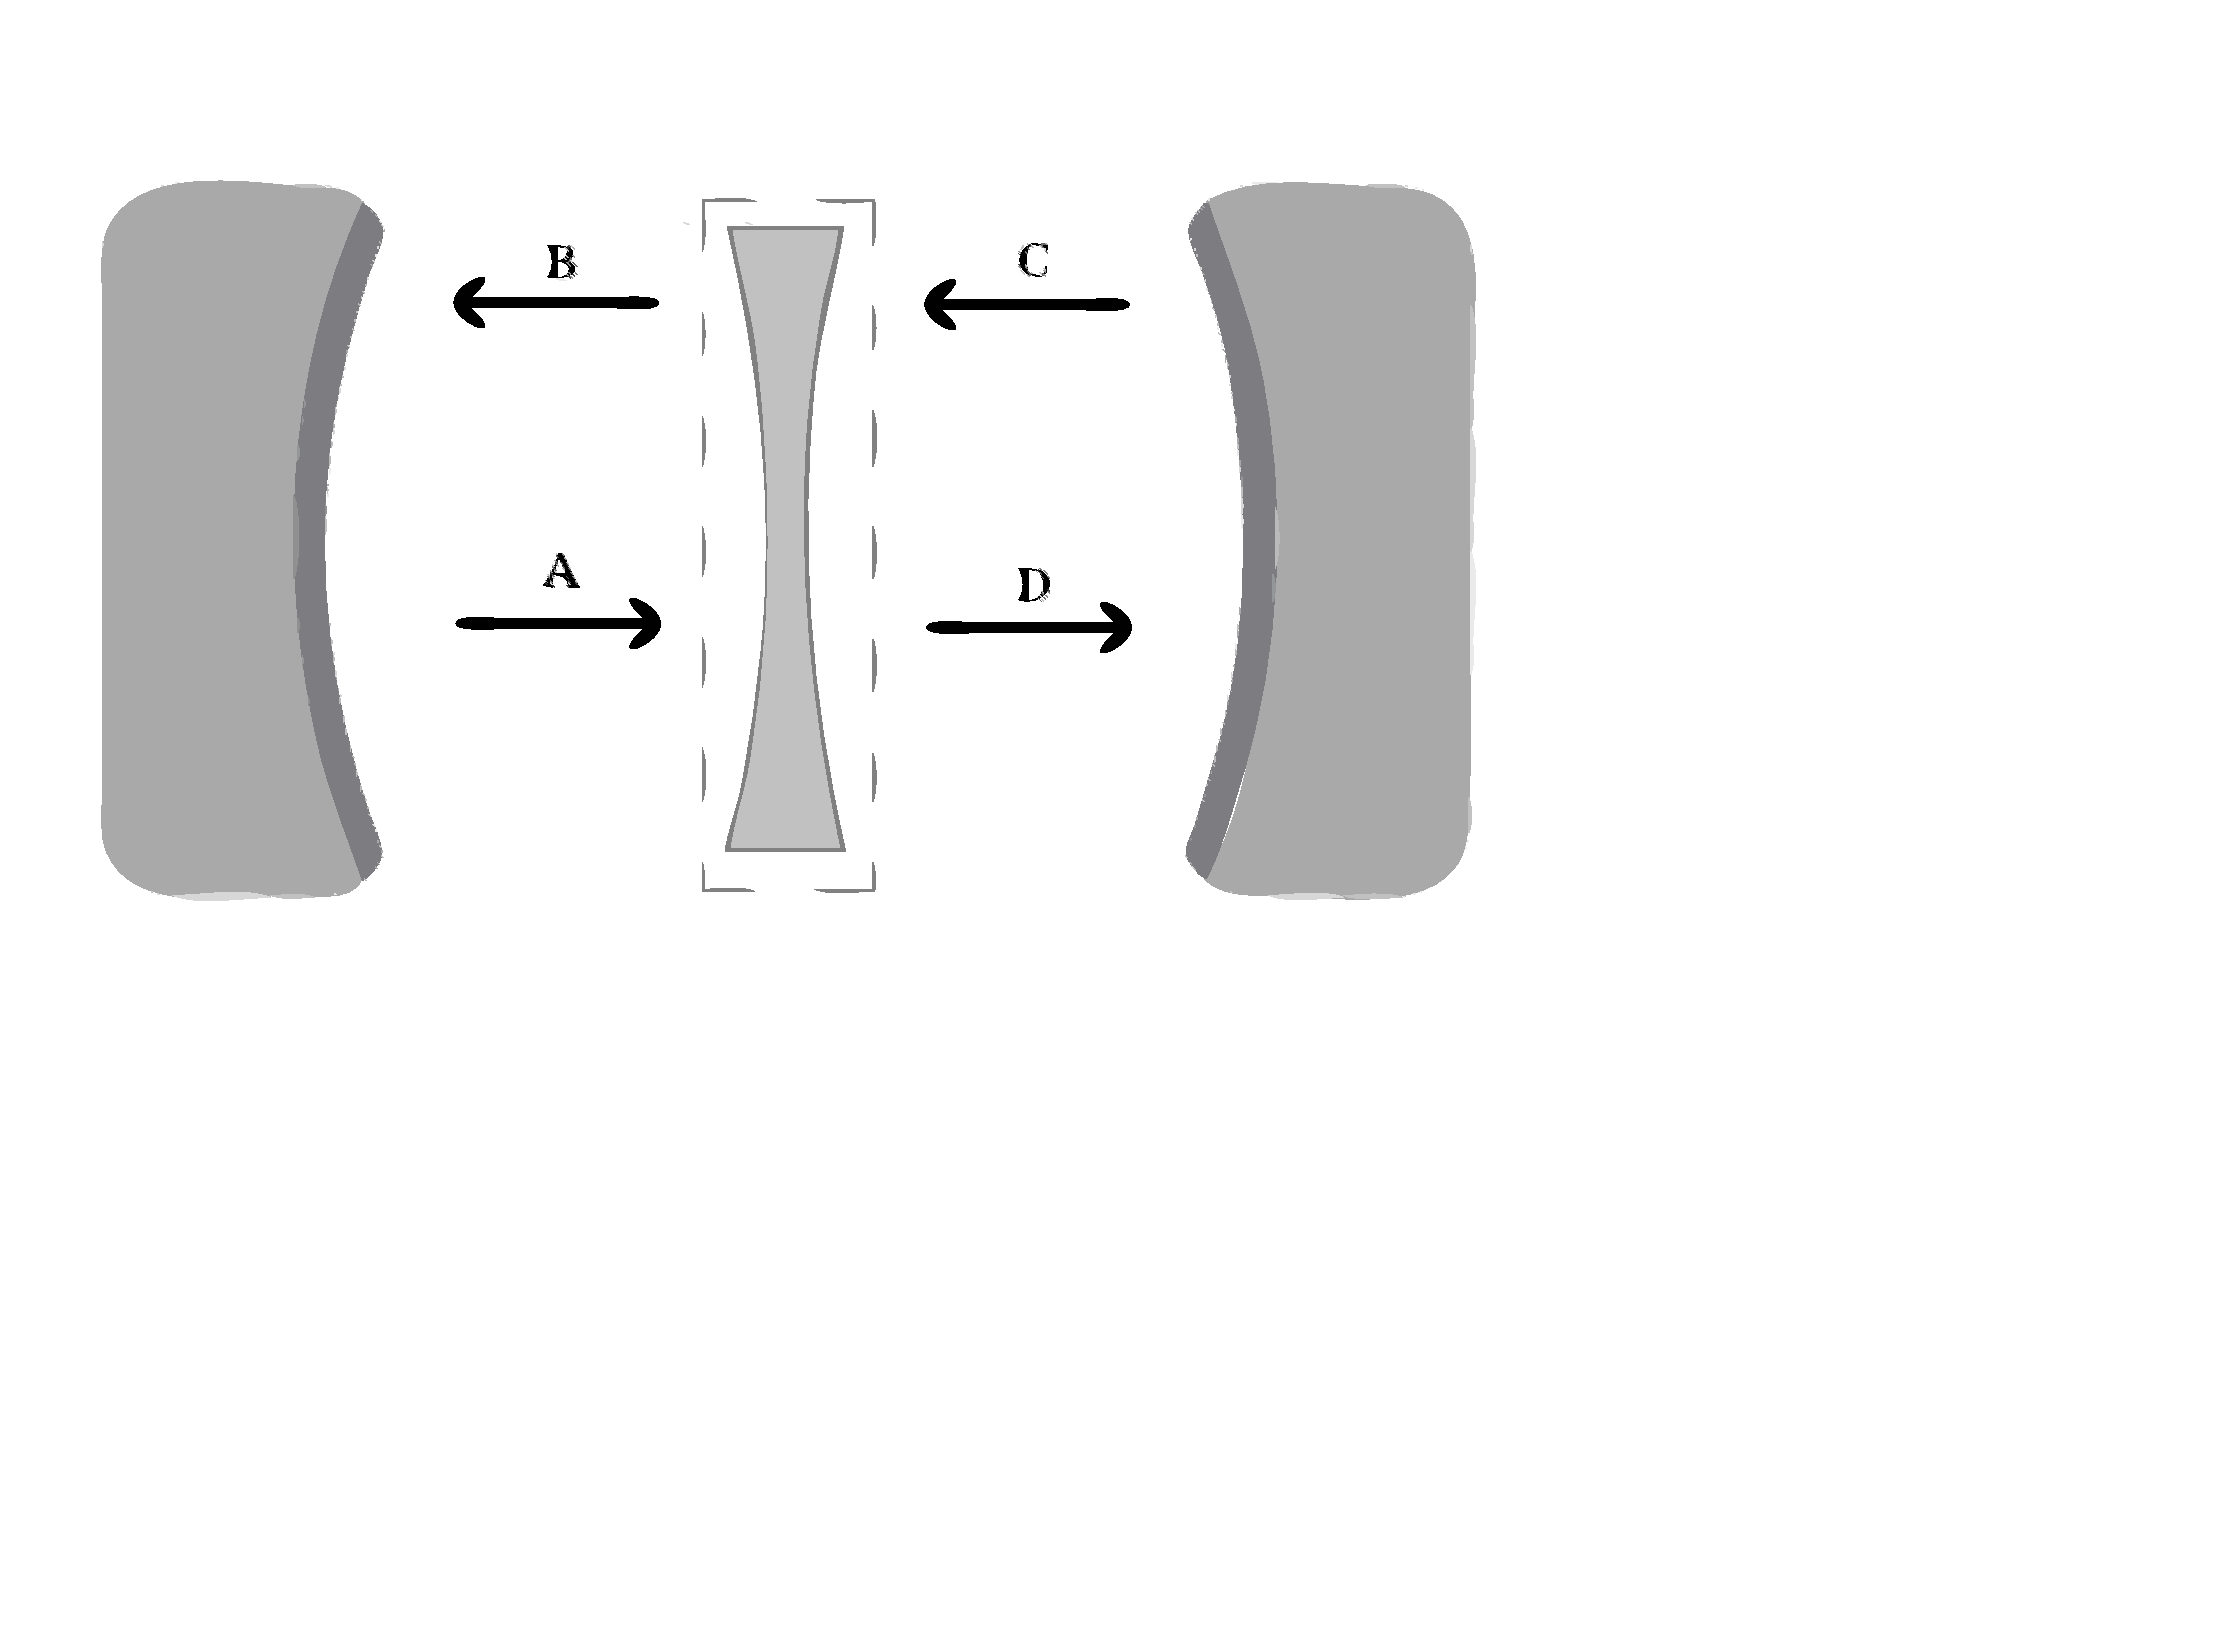
\includegraphics[width=1\columnwidth]{./Figures/GaussianPillbox}
\caption{The force is found by integrating the Maxwell stress tensor around a small pillbox containing the central mirror}
\label{fig:gaussianpillbox}
\end{figure}
%*********************************************************

\begin{equation}
F=\oint_{S}\overleftrightarrow{T}\cdot da-\varepsilon_{0}\mu_{0}\int_{V}Sd\tau
\label{stresstensor1}
\end{equation}
where $T$ is the Maxwell stress tensor defined as

\begin{equation}
T_{xx}=\frac{\varepsilon_{0}}{2}\left(\mathcal{E}_{x}^{2}-\mathcal{E}_{y}^{2}-\mathcal{E}_{z}^{2}\right)+\frac{1}{2\mu_{0}}\left(B_{x}^{2}-B_{y}^{2}-B_{z}^{2}\right)
\label{stresstensor2}
\end{equation}


\begin{equation}
T_{xy}=\varepsilon_{0}\left(\mathcal{E}_{x}\mathcal{E}_{y}\right)+\frac{1}{\mu_{0}}\left(B_{x}B_{y}\right)
\label{stresstensor3}
\end{equation}
$S$ in Eq.\ (\ref{stresstensor1}) is the poynting vector, which is zero for a stationary system.  As we are only considering the stationary modes of the system this term drops out.
If we write the modes to the left and to the right of the dielectric
slab respectively as

\begin{equation}
\mathcal{E}_{L}=\mathcal{E}_{1}e^{ikx}+\mathcal{E}_{2}e^{-ikx}
\label{Efieldleft}
\end{equation}


\begin{equation}
\mathcal{E}_{R}=\mathcal{E}_{3}e^{ikx}+\mathcal{E}_{4}e^{-ikx}
\label{EfieldRight}
\end{equation}

We then arrive at the force per unit area $F$ 

\begin{equation}
F=\frac{\varepsilon_{0}}{2}\left(\left|\mathcal{E}_{1}\right|^{2}+\left|\mathcal{E}_{2}\right|^{2}-\left|\mathcal{E}_{3}\right|^{2}-\left|\mathcal{E}_{4}\right|^{2}\right)
\label{force1}
\end{equation}

To proceed we require the amplitudes $\mathcal{E}_{1}$, $\mathcal{E}_{2}$, $\mathcal{E}_{3}$, $\mathcal{E}_{4}$. What we have instead is an analytic solution for the amplitudes
of the two standing waves to the left and to the right of the atom as is given by Eq.\ (\ref{A/B}).
If we rewrite the standing wave as the composite of two traveling waves moving in opposite direction, then we require $\mathcal{E}_{Lm}=2\mathcal{E}_{1}=2\mathcal{E}_{2}$, and $\mathcal{E}_{Rm}=2\mathcal{E}_{3}=2\mathcal{E}_{4}$.
Plugging this into Eq.\ (\ref{force1}) we obtain

\begin{eqnarray}
F&=&\frac{\varepsilon_{0}}{4}\left(\left|\mathcal{E}_{Lm}\right|^{2}-\left|\mathcal{E}_{Rm}\right|^{2}\right)\nonumber \\ &=&\left(\frac{\varepsilon_{0}}{4}\left|\mathcal{E}_{Rm}\right|^{2}\right)\left(\left|\frac{\sin(k_{m}L_{2})}{\sin(k_{m}L_{1})}\right|^{2}-1\right)
\label{force2}
\end{eqnarray}

Here we have made use of Eq.\ (\ref{A/B}. The second factor in Eq.\ (\ref{force2}) tells us that the force is proportional to the amplitude ratio between the modes on the left and right of the atom as is expected with radiative pressure. The first factor is more interesting, and tells us that it is also proportional to the energy of the field. The energy per unit area $E$ for the cavity system without the central mirror is

\begin{equation}
E=\intop_{0}^{L}\frac{\varepsilon_{0}\left|\mathcal{E}\right|^{2}}{2}dl=\frac{\varepsilon_{0}\left|\mathcal{A}_{Rm}\right|^{2}L}{4}
\label{energydensity1}
\end{equation}
 
Here we used the fact that without a central mirror $\mathcal{A}_{Lm}=\mathcal{A}_{Rm}=\mathcal{E}$. It is crucial to note that in using Eq.\ (\ref{energydensity1}) we have decided to ignore energy stored in the medium itself.  Later in this section we will revisit this choice and discuss its consequences.  
Substituting this back into Eq.\ (\ref{force2}) gives

\begin{equation}
F=\frac{E}{L}\left(\left|\frac{\sin(k_{m}L_{2})}{\sin(k_{m}L_{1})}\right|^{2}-1\right)
\label{Minkkowskiforce1}
\end{equation}

As we are interested in determining the average force per photon, we divide Eq.\ (\ref{Minkkowskiforce1}) by the number of photons $n_{photon}$.  It is assumed that the total number of photons in the cavity is conserved during motion of the mirror.  

\begin{equation}
n_{\mathrm{photon}}=\frac{E}{\hbar ck_0}
\label{photonnumber}
\end{equation}

This gives the average force per photon.

\begin{equation}
F=\frac{\hbar ck_0}{L}\left(\left|\frac{\sin(k_{m}L_{2})}{\sin(k_{m}L_{1})}\right|^{2}-1\right)
\label{Minkowskiforce2}
\end{equation}

We gain better intuition by noting that for very small $a$ we can approximate the amplitude ratio factor in Eq.\ (\ref{Minkowskiforce2}) to first order 

\begin{equation}
\left|\frac{\sin(k_{m}L_{2})}{\sin(k_{m}L_{1})}\right|^{2}\approx\frac{\pm\frac{\varepsilon_{0}L}{a m\pi}-\frac{1}{2}\sin(m\pi\frac{\triangle L}{L})}{\pm\frac{\varepsilon_{0}L}{a m\pi}+\frac{1}{2}\sin(m\pi\frac{\triangle L}{L})}
\label{amplitudeapproximation}
\end{equation}
for odd and even $m$ respectively. Substituting this into Eq.\ (\ref{Minkowskiforce2}) and simplifying yields

\begin{eqnarray}
F&=&\frac{\hbar ck_0}{L}\frac{\pm\frac{\varepsilon_{0}L}{a m\pi}-\frac{1}{2}\sin(m\pi\frac{\triangle L}{L})-\left(\pm\frac{\varepsilon_{0}L}{a m\pi}+\frac{1}{2}\sin(m\pi\frac{\triangle L}{L})\right)}{\pm\frac{\varepsilon_{0}L}{a m\pi}+\frac{1}{2}\sin(m\pi\frac{\triangle L}{L})} \nonumber \\
&\thickapprox &\mp\frac{\hbar ck_0}{L}\frac{\sin(m\pi\frac{\triangle L}{L})}{\frac{\varepsilon_{0}L}{a m\pi}}
\label{Minkowskiforce3}
\end{eqnarray}

We therefore may write the optical areal force per photon as 

\begin{equation}
F_{\mathrm{Min}}=\mp\hbar c\frac{a m^{2}\pi^{2}}{\varepsilon_{0}L^{3}}\sin(m\pi\frac{\triangle L}{L})
\label{Minkowskiforce4}
\end{equation}
for odd/even $m$ respectively.  We have written the force here with a subscript, foreshadowing results from the next segment.

Let us now retrace our steps in the derivation of the force.  We began with the Maxwell stress tensor ( see Eq.\ (\ref{stresstensor2})) and proceeded to rewrite the force in terms of the amplitude ratio (Eq.\ (\ref{force2})).  We then innocently used Eq.\ (\ref{energydensity1}) to eliminate the amplitude $\mathcal{E}_{Rm}$ in Eq.\ (\ref{force2}) in favor of writing the force in terms of the energy density $E$. As was previously mentioned, in doing so we have chosen to ignore the electromagnetic energy stored in the polarization of the medium \cite{griffiths}. Let us now go back and take into account the energy stored in polarization. We use the electric displacement $D$, and rewrite the energy density Eq.\ (\ref{energydensity1}) as \cite{griffiths}

\begin{equation}
E_{\mathrm{total}}=\intop_{0}^{L}\frac{D\cdot \mathcal{E}}{2}dl=\frac{n_{r}^{2}\varepsilon_{0}\left| \mathcal{E}_{Rm}\right|^{2}L}{4}
\label{energydensity2}
\end{equation}

where $D=\varepsilon \mathcal{E}$ and $n_{r}$ is the refractive index of the system as was found in Eq.\ (\ref{refractiveindex}).
Using this energy in Eq.\ (\ref{force2}) we obtain

\begin{equation}
F_{\mathrm{Abr}}=\frac{E}{n_{r}^{2}L}\left(\left|\frac{\sin(k_{m}L_{2})}{\sin(k_{m}L_{1})}\right|^{2}-1\right)
\label{Abrahamforce1}
\end{equation}

We have now labeled this force with a different subscript to distinguish it from Eq.\ (\ref{Minkowskiforce4}).  
Following the same logic used to obtain Eq.\ (\ref{Minkowskiforce4}) we arrive at 

\begin{equation}
F_{\mathrm{Abr}}=\mp\hbar c\frac{a m^{2}\pi^{2}}{\varepsilon_{0}n_{r}^{2}L^{3}}\sin(m\pi\frac{\triangle L}{L})
\label{Abrahamforce2}
\end{equation}

Eq.\ (\ref{Abrahamforce2}) gives the force on the central mirror as a function of the total electromagnetic field energy density.  This is in contrast to Eq.\ (\ref{Minkowskiforce4}), in which we only selected for the force due to free electromagnetic fields.  As we shall see in Section \ref{sec:Energy} this variance leads one to either realizing the Minkowski, or Abraham energy-momentum.  



\section{Energy and Momentum}
\label{sec:Energy}

We want to determine how much energy is required to realize a given mirror configuration.  We will use this as a check to confirm that the inclusion of polarization energy leads to Abraham momentum, while neglecting it will give Minkowski. It is assumed that the polarizbility factor $\alpha$ is very small, and we make use of the analytic results obtained in Sections \ref{sec:AnalyticExpressions} and \ref{sec:force}. The work-energy theorem tells us how much energy must be used in moving the central mirror to some position $\triangle L$.

\begin{equation}
\mathrm{Work}=-\int Fdx
\label{workenergy1}
\end{equation}


We first tackle the energy required to assemble the system by assuming the force is due to the free fields $F_{Min}$. We begin by considering the case in which $m$ is odd.

\begin{eqnarray}
\mathrm{Work}&=&-\int F_{Min}\frac{d\left(\triangle L\right)}{2} \nonumber \\
&=&\int_{0}^{\triangle L}\hbar c\frac{\alpha m^{2}\pi^{2}}{2L^{3}}\sin(m\pi\frac{\triangle L'}{L})d\left(\triangle L'\right) \nonumber \\
&=&-\hbar\frac{m\pi}{L}\left[\frac{\alpha}{2L}\left(\cos(m\pi\frac{\triangle L}{L})-1\right)\right]
\label{MinEnergy1}
\end{eqnarray}

What Eq.\ (\ref{MinEnergy1}) gives us is the energy per photon required to move the mirror from a central position $\triangle L=0$ , to some other position $\triangle L$.  By subtracting out this extracted energy from the initial configuration energy, we are able to arrive at an expression for the energy per photon remaining in the system.  When the mirror is in the central position, the odd mode does not "see" the mirror. The starting energy of the configuration is nothing but the initial photon energy $\hbar\omega_{0}=\hbar c\frac{n\pi}{L}$.  By subtracting Eq.\ (\ref{MinEnergy1}) from the initial energy, we find the change in energy for a given mirror configuration to be


\begin{equation}
E_{\mathrm{photon}}=\hbar c\frac{n\pi}{L}+\hbar\frac{n\pi}{L}\left[\frac{\alpha}{2L}\left(\cos(n\pi\frac{\triangle L}{L})-1\right)\right]
\label{MinEnergy2}
\end{equation}

Using Eq.\ (\ref{refractiveindex})

\begin{equation}
E_{\mathrm{photon}}=\hbar c\frac{n\pi}{L}\left[+\frac{\alpha}{2L}\left(\cos(n\pi\frac{\triangle L}{L})-1\right)+1\right]=\hbar ck_{0}n_{r}
\label{AbrEnergy4}
\end{equation}


To obtain the momentum we note that the electromagnetic fields are propagating in a vacuum, and hence we divide Eq.\ (\ref{AbrEnergy4}) by $c$ to obtain the Minkowski momentum for a photon. The
importance of this derivation lies in the realization that we had the option
to either consider only the field energy, or to also include the bound electromagnetic energy of the medium. When only the energy of free fields was considered,
we ended up with the Minkowski momentum. We now show that if
one includes the polarization energy of the dielectric, the Abraham result follows.




The procedure here is exactly the same as what we have done above, but instead of using $F_{\mathrm{Min}}$, we use $F_{\mathrm{Abr}}$.


\begin{eqnarray}
\mathrm{Work}&=&-\int F_{\mathrm{Abr}}\frac{d\left(\triangle L\right)}{2}\nonumber \\
&=&\int_{0}^{\triangle L}\frac{\hbar c\frac{\alpha m^{2}\pi^{2}}{2L^{3}}\sin(m\pi\frac{\triangle L'}{L})}{\left[+\frac{\alpha}{2L}\left(\cos(m\pi\frac{\triangle L}{L})-1\right)+1\right]^{2}}d\left(\triangle L'\right) \nonumber \\
&=&-\hbar c\frac{m\pi}{L}\left[1+\frac{\alpha}{2L}\left(\cos(m\pi\frac{\triangle L}{L})-1\right)\right]^{-1} \nonumber \\
&+&\hbar c\frac{m\pi}{L}
\label{AbrEnergy1}
\end{eqnarray}


The remaining energy is therefore

\begin{eqnarray}
E_{\mathrm{photon}}&=&\hbar c\frac{m\pi}{L} -\hbar c\frac{m\pi}{L}\nonumber \\
&+&\hbar c\frac{m\pi}{2L}\left[1+\frac{\alpha}{2L}\left(\cos(m\pi\frac{\triangle L}{L})-1\right)\right]^{-1}\nonumber \\
&=&\frac{\hbar ck_{0}}{n_{r}}
\label{AbrEnergy2}
\end{eqnarray}


Dividing Eq.\ (\ref{AbrEnergy2}) by $c$ we find that we have ended up with the Abraham momentum.

The derivation for the case in which $m$ is even is similar to the odd case, with the added twist that $\triangle L=0$ no longer corresponds to a situation in which the fields don't "see" the mirror.  We must therefore adjust the initial setup such that

\begin{equation}
\cos(m\pi\frac{\triangle L}{L})+1=(q+\frac{1}{2})\pi
\label{wavenumbereqn}
\end{equation}
where $q$ is an integer.  By doing so we can follow the same strategy used for the odd case and arrive at the same conclusion.  We omit the derivation for sake of repetitiveness.


\section{Experimental Ambiguity}
\label{sec:experiment}


What does the above analysis tell us about why the Abraham and Minkowski momentum both are present in experimental findings?  Section \ref{sec:force} tells us that the disagreement arises due to an ambiguity in attributing the total force owing to one subsystem or another.  
 %The problem emerges from the fact that there are no restrictions placed on how one divides the material energy-momentum from the electromagnetic energy-momentum.%
  %In a thermodynamically closed system one must take into account both the material and electromagnetic energy-momentum \cite{pfeifer07}.  It is the total energy-momentum tensor that is responsible for the momentum transfer, and this is unambiguous. The Abraham-Minkowski momentum correspond to two choices in energy-momentum tensors for the electromagnetic division.   So why do some experiments suggest Minkowski while others suggest Abraham? %

In appendix A we show how one can map the single atom in a cavity to the $\delta$-function model.  Using this, it can be shown that the Minkowski momentum of the field is related to the canonical momentum of a single dipole while the Abraham momentum is affiliated with the kinetic momentum of the dipole.  The relationship between the kinetic and canonical momentum of a single dipole is given by \cite{hinds}

\begin{equation}
p_{\mathrm{Kinetic}}=p_{\mathrm{Canonical}}+d \times B
\label{canonicaldipole}
\end{equation}
 
We may write the second term on the right side of Eq.\ (\ref{canonicaldipole}) as 

\begin{equation}
d \times B =\frac{\varepsilon_{0} n_{r}\left(n_{r}^2-1\right)\mathcal{E}^2V}{c}
\label{dipoleterm1}
\end{equation}

Or in terms of single photons

\begin{equation}
\hbar k_{0} \left(\frac{n_{r}^2-1}{n_{r}}\right)
\label{dipoleterm2}
\end{equation}

This is precisely the difference between the Abraham Eq.\ (\ref{AbrEnergy2}) and Minkowski Eq.\ (\ref{AbrEnergy4}) momentum. 
Barnett and Hinds \cite{Hinds} attribute the difference as arising from neglecting components of the Lorentz force.  The force may be written as 
  
\begin{equation}
F=d \cdot \frac{\partial\mathcal{E}(x,t)}{\partial x} + \frac{\partial}{\partial t}\left(d \times B \right)
\label{hindsforce}
\end{equation}

By considering only the first term on the right of Eq.\ (\ref{hindsforce})they obtain the Minkowski result, whereas Abraham is realized if both terms are accounted for. As applied to our cavity system, the second term in equation Eq.\ (\ref{hindsforce}) represents the contribution from the polarization energy stored in the atom. Therefore we see that in diffraction experiments, as the field intensity is more or less static, the second term becomes negligible and we obtain the Minkowski result.  In experiments in which we have an electromagnetic pulse incident on a dielectric block, the second term can no longer be neglected, and as is shown in \cite{Hinds}, is twice as large in magnitude as the first term yielding Abraham.  Therefore the form of momentum observed depends on whether or not this second term is present or not.  For us this suggests that the energy change in the polarized atoms may only be neglected when the time $t$ that the atom is acted on by the field satisfies


\begin{equation}
\Delta \left(d \times B \right) \ll  \left(d \cdot \frac{\partial\mathcal{E}(x,t)}{\partial x}\right)t)
\label{timecompare}
\end{equation}


%What this tells us is that \cite{hinds}%

%\begin{equation}
%M\dot{r}_{\mathrm{atom}} +p_{\mathrm{Abraham}} =P_{\mathrm{atom}} + %p_{\mathrm{Minkowski}}
%\label{canonicalkinetic}
%\end{equation}

%Note that the total momentum %
%making up either side of Eq.\ (\ref{canonicalkinetic}) is fixed.  Consider now the diffraction experiment done by Ketterle's group \cite{ketterle}.  As it is the canonical momentum of the atom used in deriving the deBroglie wavelength, one expects that the associated field momentum in a diffraction experiment to be the Minkowski momentum.  This is indeed what they find in their analysis.  On the other hand, an experiment such as that proposed by Loudon \cite{loudon2} in which the torque on a transparent disc is considered, it is the kinetic momentum which is relevant.  Using a conservation of momentum argument here must yield the Abraham momentum for the field, corroborating Loudon's conclusion.%

\section{Conclusion}
\label{sec:conclusion}

We'll finish this later...
The Minkowski-Abraham paradox is shown to originate from interpreting the momentum transfer as arising from different components of the system energy. By including or neglecting the energy bound in the polarization one either obtains the Abraham or the Minkowski field momentum.  
  
Here we calculate the amplification effect that the cavity has on the refractive index of an atom.  From \cite{cohentannoudji} the average refractive index $n_{free}$ of a an atom in free space is given by

\begin{equation}
n_{\mathrm{free}}\approx 1+\frac{\alpha_{p}N}{2\varepsilon_{0}}
\end{equation}

where $N$ is the density.  For comparison sake, we take $N=1/L$.  Comparing this to Eq.\ (\ref{refractiveindex}) we see that the refractive index $n_{r}$ of the cavity-atom system is at most double the value of the free refractive index. 

\section{A Connecting the Maxwell Stress Tensor and the Dipole Force}
\label{sec:AppendixAMaxwellvsQOforce}


In this appendix, we connect the microscopic description of optical forces on atoms \cite{cohentannoudji} with the classical derivation obtained in Section \ref{sec:force}.  
This relationship will link the $\delta$-function factor $a$ in Eq.\ (\ref{perm}) with the polarizability of an atom. We begin by examining the force 
derived using the Maxwell stress tensor.  Suppose we have a dielectric slab, which we approximate with a $\delta$-function, interacting with two opposing plane waves. 
From Eq.\ (\ref{force1}) we can write the force as

\begin{equation}
F=\frac{\varepsilon_{0}}{2}\left(\left|\mathcal{E}_{1}\right|^{2}+\left|\mathcal{E}_{2}\right|^{2}-\left|\mathcal{E}_{3}\right|^{2}-\left|\mathcal{E}_{4}\right|^{2}\right)
\label{Gaussianforce}
\end{equation}

Let us rewrite the outgoing fields $\mathcal{E}_{1}$ and $\mathcal{E}_{4}$ as a linear combination of the incoming fields $\mathcal{E}_{2}=\mathcal{E}_{\mathrm{left}}e^{ikx+i\phi}$ 
and $\mathcal{E}_{3}=\mathcal{E}_{\mathrm{right}}e^{-ikx}$ (see Figure \ref{fig:gaussianpillbox}).

\begin{equation}
\mathcal{E}_{1}=r\mathcal{E}_{2}+t\mathcal{E}_{3}
\label{E1}
\end{equation}


\begin{equation}
\mathcal{E}_{4}=t\mathcal{E}_{2}+r\mathcal{E}_{3}
\label{E4}
\end{equation}

where the reflectivity $r$ and the transmission $t$ for the $\delta$-model are given by \cite{us}

\begin{equation}
r=\frac{i\frac{k a}{2\varepsilon_{0}}}{1-\frac{ik a}{2\varepsilon_{0}}}
\label{reflectivity}
\end{equation}


\begin{equation}
t=\frac{1}{1-\frac{ik a}{2\varepsilon_{0}}}
\label{transmission}
\end{equation}

Substituting these equations into Eq.\ (\ref{force1}) yields

%\frac{\varepsilon_{0}}{2}
\begin{eqnarray}
F&=&\frac{\frac{\varepsilon_{0}}{2}\left|\frac{k a}{2\varepsilon_{0}}\right|^{2}}{\left|1-\frac{ika}{2\varepsilon_{0}}\right|^{2}}\left|\mathcal{E}_{\mathrm{left}}\right|^{2}+\frac{\frac{\varepsilon_{0}}{2}}{\left|1-\frac{ika}{2\varepsilon_{0}}\right|^{2}}\left|\mathcal{E}_{\mathrm{right}}\right|^{2} \nonumber \\
&+&\frac{i\frac{\varepsilon_{0}ka}{4\varepsilon_{0}}}{\left|1-\frac{ika}{2\varepsilon_{0}}\right|^{2}}\mathcal{E}_{\mathrm{left}}\mathcal{E}_{\mathrm{left}}e^{2ikx+i\phi}\nonumber \\
&-&\frac{i\frac{ka^{*}}{4}}{\left|1-\frac{ika}{2\varepsilon_{0}}\right|^{2}}\mathcal{E}_{\mathrm{left}}\mathcal{E}_{\mathrm{right}}e^{-2ikx-i\phi} \nonumber \\
&+&\frac{\varepsilon_{0}}{2}\left|\mathcal{E}_{\mathrm{left}}\right|^{2}-\frac{\varepsilon_{0}}{2}\left|\mathcal{E}_{\mathrm{right}}\right|^{2}-\frac{\frac{\varepsilon_{0}}{2}\left|\frac{ka}{2\varepsilon_{0}}\right|^{2}}{\left|1-\frac{ika}{2\varepsilon_{0}}\right|^{2}}\left|\mathcal{E}_{\mathrm{right}}\right|^{2} \nonumber \\
&-&\frac{\frac{\varepsilon_{0}}{2}}{\left|1-\frac{ika}{2\varepsilon_{0}}\right|^{2}}\left|\mathcal{E}_{\mathrm{left}}\right|^{2}-\frac{i\frac{ka}{4}}{\left|1-\frac{ika}{2\varepsilon_{0}}\right|^{2}}\mathcal{E}_{\mathrm{left}}\mathcal{E}_{\mathrm{right}}e^{-2ikx-i\phi} \nonumber \\
&+&\frac{i\frac{ka^{*}}{4}}{\left|1-\frac{ika}{2\varepsilon_{0}}\right|^{2}}\mathcal{E}_{\mathrm{left}}\mathcal{E}_{\mathrm{right}}e^{2ikx+i\phi}
\label{f1}
\end{eqnarray}

Here $a$ is a complex parameter which we break up in its real and imaginary components $a=a_{1}+ia_{2}$. Simplifying the expression above yields

\begin{eqnarray}
F &=&-\frac{ka_{1}\mathcal{E}_{\mathrm{left}}\mathcal{E}_{\mathrm{right}}\sin\left(2kx+\phi\right)}{\left|1-\frac{ika}{2\varepsilon_{0}}\right|^{2}} \nonumber \\
&+&\frac{\frac{ka_{2}}{2}\left(\left|\mathcal{E}_{\mathrm{left}}\right|^{2}-\left|\mathcal{E}_{\mathrm{right}}\right|^{2}\right)}{\left|1-\frac{ika}{2\varepsilon_{0}}\right|^{2}} \nonumber \\
&+&\frac{\varepsilon_{0}\left|\frac{ka}{2\varepsilon_{0}}\right|^{2}\left(\left|\mathcal{E}_{\mathrm{left}}\right|^{2}-\left|\mathcal{E}_{\mathrm{right}}\right|^{2}\right)}{\left|1-\frac{ika}{2\varepsilon_{0}}\right|^{2}}
\label{f2}
\end{eqnarray}



where $\phi$ is the phase difference between the two incoming waves at $x=0$. Let us examine Eq.\ (\ref{f2}) term by term to gain a better understanding
of what each term represents. The first term, which we label as $F_{1}$, is the reactive part of the force more commonly known as the dipole force. To see this let us consider the standard reactive force on an atom as given by Cohen-Tannoudji \cite{cohentannoudji} for a field of the form $\mathcal{E}(x)=\mathcal{E}_{\mathrm{left}}e^{ikx+i\phi}+\mathcal{E}_{\mathrm{right}}e^{-ikx}$ 

\begin{equation}
F_{\mathrm{reactive}}=-\frac{\hbar\Delta}{4}\frac{\overrightarrow{\nabla}\Omega^{2}}{\frac{\Gamma^{2}}{4}+\Delta^{2}+\frac{\Omega^{2}}{2}}=\frac{1}{4}\alpha_{1}\nabla \mathcal{E}^{2}
\label{cohentannoudjiforce1}
\end{equation}

Here $\Omega$ is the atomic Rabi frequency, $\Gamma$ is the spontaneous decay rate, $d$ is the dipole coherence, and $\Delta$ is the detuning.
We also introduce $\alpha_{1}$ as the real component of the atomic polarizibility given by

\begin{equation}
\alpha=\frac{-\Delta\left|d\right|^{2}}{\hbar\left[\frac{\Gamma^{2}}{4}+\Delta^{2}+\frac{\Omega^{2}}{2}\right]}\approx\frac{-\left|d\right|^{2}}{\hbar\Delta}
\label{polarizibility1}
\end{equation}

One finds that for $\mathcal{E}(x)=\mathcal{E}_{\mathrm{left}}e^{ikx+i\phi}+\mathcal{E}_{\mathrm{right}}e^{-ikx}$

\begin{equation}
\nabla \mathcal{E}^{2}=-4k\mathcal{E}_{\mathrm{left}}\mathcal{E}_{\mathrm{right}}\sin\left(2kx+\phi\right)
\label{gradiantE}
\end{equation}
Substituting this back into Eq.\ (\ref{cohentannoudjiforce1}) we get

\begin{equation}
F_{\mathrm{reactive}}=-\alpha k\mathcal{E}_{\mathrm{left}}\mathcal{E}_{\mathrm{right}}\sin\left(2kx+\phi\right)
\label{cohentannoudjiforce2}
\end{equation}

We now compare Eq.\ (\ref{cohentannoudjiforce2}) to the first term $F_{1}$ of Eq.\ (\ref{f2}). If we are considering a single atom in the dispersive regime, then
$a$ may be assumed very small. We may therefore approximate $F_{1}$ to first order in $a$ 

\begin{equation}
F_{1}\approx-a_{1} \mathcal{E}_{\mathrm{left}}\mathcal{E}_{\mathrm{right}}\sin\left(2kx+\phi\right)
\label{cohentannoudjiforce3}
\end{equation}

Comparing Eq.\ (\ref{cohentannoudjiforce2}) with Eq.\ (\ref{cohentannoudjiforce3}) we see that for an atom, $\alpha_{1}=a_{1}$, and that indeed $F_{1}$ is the reactive component of the optical force. 

%***************************figure**********************
\begin{figure}
\includegraphics[width=1\columnwidth]{./Figures/MaxwellForcevsCoherentForce}
\caption{This plot compares the complete force obtained using the Maxwell stress tensor (red) against the reactive component - the first term $F_{1}$ of Eq.\ (\ref{f2}) (blue).  Here $alpha=10^{-8}$ was used.  It is seen that for small $alpha$, the other two components of Eq.\ (\ref{f2}) may be neglected.}
\label{fig:forcecompare}
\end{figure}
*********************************************************

 Let us now return to Eq.\ (\ref{f2}) and consider the second term $F_{2}$ in the equation.  This term can be shown to be nothing more than the dispersive force.  Following a similar scheme to that used above we have 


\begin{equation}
F_{2}=\frac{\frac{1}{2}ka_{2}\left(\left|\mathcal{E}_{\mathrm{left}}\right|^{2}-\left|\mathcal{E}_{\mathrm{right}}\right|^{2}\right)}{\left|1-\frac{ik\alpha}{2}\right|^{2}}
\label{secondforce1}
\end{equation}

For small $a$ we approximate $F_{2}$ to first order

\begin{equation}
F_{2}\approx\frac{1}{2}ka_{2}\left(\left|\mathcal{E}_{\mathrm{left}}\right|^{2}-\left|\mathcal{E}_{\mathrm{right}}\right|^{2}\right)
\label{secondforce2}
\end{equation}

We now wish to compare this to the dispersive force as given by Cohen-Tannoudji \cite{cohentannoudji}. The dispersive force felt by an atom under the influence of a field
of the form $\mathcal{E}(x)=\mathcal{E}_{\mathrm{left}}e^{ikx+i\phi}+\mathcal{E}_{\mathrm{right}}e^{-ikx}$ is given by

\begin{eqnarray}
F_{\mathrm{dispersive}e}&=&-\hbar\Gamma\left(\overrightarrow{\nabla}\phi(\overrightarrow{r})\right)\frac{\Omega^{2}}{\Gamma^{2}+4\Delta^{2}+2\Omega^{2}} \nonumber \\
&=&\left(\left|\mathcal{E}_{\mathrm{left}}\right|^{2}-\left|\mathcal{E}_{\mathrm{right}}\right|^{2}\right)\frac{k\left|d\right|^{2}\Gamma}{4\hbar\Delta^{2}}
\label{dispersive1}
\end{eqnarray}

The imaginary component of the polarizibility of an atom is \cite{cohentannoudji}


\begin{equation}
\alpha_{2}=\frac{\frac{\Gamma}{2}\left|d\right|^{2}}{\hbar\left[\frac{\Gamma^{2}}{4}+\Delta^{2}+\frac{\Omega^{2}}{2}\right]}\approx\frac{\Gamma d^{2}}{2\hbar\Delta^{2}}
\label{polarizibility2}
\end{equation}

Thus we can rewrite the dispersive force as

\begin{equation}
F_{\mathrm{dispersive}}=\frac{\alpha_{2}k}{2}\left(\left|\mathcal{E}_{\mathrm{left}}\right|^{2}-\left|\mathcal{E}_{\mathrm{right}}\right|^{2}\right)
\label{dispersive2}
\end{equation}


Comparing Eq.\ (\ref{dispersive2}) with Eq.\ (\ref{secondforce2}) and see that $\alpha_{2}=a_{2}$, consistent with what we found for the reactive component of the force.  Now the third component $F_{3}$ of Eq.\ (\ref{f2}) is interpreted as the radiation pressure due to incoherent scattering.  To see this we note that

\begin{equation}
R=\left|r\right|^{2}=\frac{\left|\frac{ka}{2\varepsilon}\right|^{2}}{\left|1-\frac{ika}{2\varepsilon}\right|^{2}}
\label{reflectioncoefficient}
\end{equation}

Comparing the coefficient in Eq.\ (\ref{f2}) with Eq.\ (\ref{reflectioncoefficient}) we see that indeed

\begin{equation}
F_{3}=2 R \left(\left|\mathcal{E}_{\mathrm{left}}\right|^{2}-\left|\mathcal{E}_{\mathrm{right}}\right|^{2}\right)
\label{incoherentforce}
\end{equation}

This is a second order effect in $a$ which is why it is neglected in the conventional optical force on an atom.  For higher densities however, it dominates $F_{1}$ and $F_{2}$ which explains why the radiative pressure equation of classical electrodynamics \cite{griffiths} agrees well for high density objects such as mirrors.  



%================================================================

%================================================================
\chapter{Conclusions and Outlook}
\chaptermark{Conclusions and Outlook}
%================================================================


In this final chapter,...


%================================
\section{Conclusions}
Why is it that so many experiments tend to favor the Minkowski form and that there are only a couple claims to Abraham? The reason lies with the Abraham force $f^A=\varepsilon_0\left(\mathbf{\varepsilon_r}-1\right)\frac{\partial}{\partial t}\mathbf{E}\times\mathbf{B}$. As we saw in Section \ref{sec:forces}, this only becomes relevant in certain situations.  We saw that this force averages to zero over an optical cycle. This makes it notoriously difficult to see in experimentation. The momentum transferred however, is only dependent on the initial and final amplitude of the field.  If one considers the momentum gained from the field due to a field which is initially at zero and is then turned up to some maximal strength $E_{\mathrm{max}}$, one finds the Abraham contribution is twice as much as that due to the gradient force.  Of course for a pulsed field, the Abraham force will contribute zero total momentum as the initial and final amplitudes are both the same.  The reason why the Abraham force has been so elusive, is because we have been doing the wrong experiments. Recently, Rikken and Tiggelen [2] claim to have seen the Abraham force.  In their experiment however, they used a static magnetic field and applied an alternating voltage perpendicular to the magnetic field.  As the Abraham force is applied at a normal angle to the $E$ and $B$ fields, they only measured the force acting in this direction and therefore were able to avoid the issue of having the Abraham force masked by the gradient force.  What we are looking for however is an example in which one observes the Abraham momentum in an electromagnetic field.  Let us first go through some of the big experiments in which the authors make claims to the Minkowski form.
\\
The first experiment to consider was performed by Pritchard and Ketterle \cite{ketterle}.  They used an elongated $^{87}Rb$ Bose-Einstein condensate contained in a magnetic trap.  They used a $\lambda=780 nm$ standing wave pulse which acted for $5 \mu s$ to out couple approximately $5\%$ of the atoms.  After waiting $600 \mu s$ a second pulse was applied which out coupled another group of atoms, interfering with the first group.  Using ballistic imaging they were able to resolve the momentum states and conclude that the atoms had acquired a momentum kick proportional to the refractive index of the gas, thus corroborating Minkowki's claim.  We immediately see the issue here however.  By pulsing the standing wave, they have ensured that the Abraham force will contribute nothing after the full pulse cycle.  

So what is the message to take home from this?  Let's go back and take a look at Poynting's theorem in the Minkowski and the Abraham representation.  In the Minkowski representation we have
\begin{equation}
\mathbf{f}+\frac{\partial}{\partial t}\left[\mathbf{D}\times\mathbf{B}\right]=\nabla\cdot\left(\mathbf{E}\mathbf{D}+\mathbf{H}\mathbf{B}-\frac{1}{2}\mathbf{I}\left(\mathbf{D}\cdot\mathbf{E}+\mathbf{H}\cdot\mathbf{B}\right)\right)
\end{equation}
\\
where we identify $\mathbf{f}$ with the mechanical momentum of system.  What this equation is telling us is that 
\begin{equation}
\frac{\partial}{\partial t}\left(\mathbf{P}_{\mathrm{mechanical}}\right)+\frac{\partial}{\partial t}\left(\mathbf{P}_{\mathrm{electromagnetic}}\right)=\nabla\cdot\mathbf{W}_{\mathrm{total}}
\end{equation}
where $\mathbf{P}_{\mathrm{mechanical}}$ is the mechanical momentum of the material, $\mathbf{P}_{\mathrm{electromagnetic}}$ is the electromagnetic momentum, and $\mathbf{W}_{\mathrm{total}}$ is the total work done.  Now just as we had previously done in the Energy Momentum section, we and subtract  
$\varepsilon_0\left(\mathbf{\varepsilon_r}+1\right)\frac{\partial}{\partial t}\mathbf{E}\times\mathbf{B}$ from both sides.  This gives us
\begin{equation}
\tilde{\mathbf{f}}+\frac{\partial}{\partial t}\frac{\mathbf{E}\times\mathbf{H}}{c^2} =\nabla\cdot\left(\mathbf{E}\mathbf{D}+\mathbf{H}\mathbf{B}-\frac{1}{2}\mathbf{I}\left(\mathbf{D}\cdot\mathbf{E}+\mathbf{H}\cdot\mathbf{B}\right)\right)
\end{equation}
where $\tilde{\mathbf{f}}=\mathbf{f}+\varepsilon_0\left(\mathbf{\varepsilon_r}+1\right)\frac{\partial}{\partial t}\mathbf{E}\times\mathbf{B}$.  Now in the Abraham representation, all we have done is identified $\tilde{\mathbf{f}}$ with $\frac{\partial}{\partial t}\mathbf{P}_{\mathrm{mechanical}}$ and $\frac{\mathbf{E}\times\mathbf{H}}{c^2}$ with $\frac{\partial}{\partial t}\mathbf{P}_{\mathrm{electromagnetic}}$.  So how does this fit in with our findings that the Abraham force $\varepsilon_0\left(\mathbf{\varepsilon_r}+1\right)\frac{\partial}{\partial t}\mathbf{E}\times\mathbf{B}$ is usually negligible?  Consider that experiments will measure the momentum impulse $\tilde{\mathbf{f}}$ of the atoms and since the Abraham term is so notoriously difficult to detect, they will detect the absence of this term and will therefore assume the material momentum is $\mathbf{f}$ which will lead them to the Minkowski momentum.  So what is the correct picture.  The correct picture is the Abraham representation.  Going back to the derivation of the Minkowski representation, it's clear that the material momentum only considers the free charge momentum.  The Abraham representation correctly accounts for the momentum of the bound charges which travel along with the pulse.  These bound charges are pulled towards the pulse as it approaches, and then rapidly brought to a halt as the pulse passes.  It is this ephemeral motion which is to blame for all the confusion.  




%================================
\section{Future Directions}





%================================================================


\singlespacing

%APPENDICES
\begin{appendices}
\appendixpage
\noappendicestocpagenum
%================================================================
\chapter{Appendix to Chapter 2}
\chaptermark{Appendix to Chapter 2}
\label{Appendix_for_Ch_2}
%================================================================

  
In this appendix I derive some of the fundamental results of this thesis. Details omitted in the body of the thesis are shown here.  In the first subsection I fully derive the Abraham representation and show all steps.  In the second subsection I show how to derive the direct coupling Hamiltonian from the minimal coupling representation.  Finally in the third subsection I show how one can derive the direct coupling Hamiltonian through a gauge transformation.



%==============================
\section{Appendix:Abraham Representation Expansion}
\label{App_1-1}
In this section we go through the derivation of the Abraham Hamiltonian given by Eq.\ (\ref{schrodinger2}).  Eq.\ (\ref{schrodinger3}) can be similarly derived.  The Schrodinger equation Eq.\ (\ref{schrodinger1}) is given by
\begin{eqnarray}
\mathrm{i\hbar\dot{\psi}}&=&\mathrm{\frac{1}{2M}\left(\mathbf{P}+ \mathbf{S}_A-\frac{\mathbf{m}\times\mathbf{E}}{c^2}\right)^2\,\Psi-\frac{1}{2}\alpha E^2\,\psi}\nonumber \\
&-&\mathrm{\mathbf{m}\cdot\mathbf{B}\,\psi+\left(\int\left[\frac{\epsilon_0}{2}E^2+ \frac{1}{2\mu_0}B^2\right]\,dV\right)\,\psi}
\label{schrodingerappendix1}
\end{eqnarray}
Here we have written 
\begin{equation}
\mathrm{\mathbf{S}_A=\int \left(\mathbf{D}\times\mathbf{B}\right) \, dV}
\end{equation}
We then apply the a unitary transformation to the wave function and write $\psi$ as
\begin{equation}
\mathrm{\psi=\Psi\exp{\left[-\frac{\mathrm{i}}{\mathrm{\hbar}}\int_{\gamma[0,\mathbf{r}]}\mathbf{S}_M\cdot d\mathbf{r}'\right]}}
\label{abrahamrepappendix}
\end{equation}
Where the integral is a path integral between $[0,\mathrm{\mathbf{r}}]$
This yields
\begin{eqnarray}
&&\mathrm{\mathrm{i}\mathrm{\hbar}\dot{\Psi}+\Psi\,\left(\frac{\partial}{\partial t}\mathrm{\int_0^\mathbf{x} \mathbf{S}_A \, \mathrm{dx'}}\right)}\nonumber \\
&=&\mathrm{-\hbar^2(\nabla^2\Psi)+2i\hbar(\mathbf{\nabla}\Psi)\mathbf{S}_A+\Psi {S_A}^2+i\hbar\Psi(\mathbf{\nabla}\mathbf{S}_A)} \nonumber \\
&&\mathrm{-2i\hbar(\mathbf{\nabla}\Psi)\mathbf{S}_A-i\hbar\Psi(\mathbf{\nabla}\mathbf{S}_A)-2\Psi{\mathbf{S}_A}^2} \nonumber \\
&&\mathrm{-2i\hbar(\mathbf{\nabla}\Psi)(\mathbf{d}\times\mathbf{B})-i\hbar\Psi(\mathbf{\nabla}(\mathbf{d}\times\mathbf{B}))-2\Psi\mathbf{S}_A(\mathbf{d}\times\mathbf{B}) }\nonumber \\
&&\mathrm{+\Psi\left({\mathbf{S}_A}^2+(\mathbf{d}\times\mathbf{B})^2+2\mathbf{S}_A(\mathbf{d}\times\mathbf{B})\right)}\nonumber \\
&&\mathrm{-\Psi\int\frac{1}{2}\left(\mathbf{D\cdot E +H\cdot B}\right)\,dV}
\label{schrodingera2}
\end{eqnarray}
Here we have omitted writing out the phase factor 
\begin{equation}
\mathrm{\exp{\left[-\frac{\mathrm{i}}{\mathrm{\hbar}}\int_0^\mathbf{x}\mathbf{S}_A\,\mathrm{dx'}\right]}}
\label{phasefactor}
\end{equation}
as it appears multiplying every term and will be factored out.  Canceling terms leaves us with
\begin{eqnarray}
&&\mathrm{\mathrm{i}\mathrm{\hbar}\dot{\Psi}+\Psi\,\left(\frac{\partial}{\partial t}\mathrm{\int_0^\mathbf{x} \mathbf{S}_A \, \mathrm{dx'}}\right)}\nonumber \\
&=&\mathrm{-\hbar^2(\nabla^2\Psi) -2i\hbar(\mathbf{\nabla}\Psi)(\mathbf{d}\times\mathbf{B})-i\hbar\Psi(\mathbf{\nabla}(\mathbf{d}\times\mathbf{B}))}\nonumber \\
&&\mathrm{+\Psi(\mathbf{d}\times\mathbf{B})^2-\Psi\int\frac{1}{2}\left(\mathbf{D\cdot E +H\cdot B}\right)\,dV}
\label{schrodingera3}
\end{eqnarray}
Factoring terms, this can be rearranged into
\begin{equation}
\mathrm{i\mathrm{\hbar}\dot{\Psi}=\mathrm{\left(\frac{\left(\mathbf{P}+\mathbf{d}\times\mathbf{B}\right)^2}{2M}-\int\frac{1}{2}\left(\mathbf{D\cdot E}+\mathbf{H\cdot B}\right)\,dV-\frac{\partial}{\partial t}\int_0^\mathbf{x} \mathbf{S}_A\,\mathrm{dx'}\right)\Psi}}
\label{schrodingera4}
\end{equation}



%==============================
\newpage
\section{Appendix: The G\"{o}ppert-Mayer Transformation }
\label{App_1-2} 


We begin with the minimal coupling Hamiltonian for a system of charges interacting with an electromagnetic field
\begin{equation}
\mathrm{H(t)=\sum_{j}\frac{1}{2m_j}\left[\mathbf{p}_j-q_j \,\mathbf{A}(\mathbf{0},t)\right]^2+V_{c}(\mathbf{x})}
\label{appendixminimalhamiltonian}
\end{equation}
where $\mathbf{A}(\mathbf{x},t)$ is the vector potential, $e_j$ is the charge, and $V_{\mathrm{c}}(\mathbf{x})$ is the scalar potential energy of the system.  In the long-wavelength approximation, we have assumed the spatial variation of $\mathbf{A}(\mathbf{x},t)$ is negligible.  We therefore choose the location of the system of charges considered to be at $\mathbf{x}=0$ and set $\mathbf{A}(\mathbf{x},t)=\mathbf{A}(\mathbf{0},t)$.  The corresponding Schr\"{o}dinger equation for the minimal coupling Hamiltonian is given by
\begin{equation}
\mathrm{i\hbar \dot{\psi}(\mathbf{x},t)=\left[\sum_{j}\frac{1}{2m_j}\left[\mathbf{p}_j-q_j\, \mathbf{A}(\mathbf{0},t)\right]^2+V_{c}(\mathbf{x})\right]\psi(\mathbf{x},t)}
\label{minimalschrodinger}
\end{equation}
The unitary transformation responsible for giving rise to the electric dipole interaction (direct coupling representation) is given by the G\"{o}ppert-Mayer transformation (GMT)
\begin{equation}
\mathrm{\Theta (t)=\mathrm{\exp{\left[\frac{\mathrm{i}}{\mathrm{\hbar}}\sum_jq_j\,\mathbf{r}_j\cdot \mathbf{A}(\mathbf{0},t) \right]}=\exp{\left[\frac{\mathrm{i}}{\mathrm{\hbar}}\mathbf{d}\cdot \mathbf{A}(\mathbf{0},t) \right]}}}
\label{gmtransformation}
\end{equation}
where
\begin{equation}
\mathbf{d}=\sum_{j} e_j \,\mathbf{r}_j
\end{equation}
 We rewrite the wave function $\psi$ as
\begin{equation}
\mathrm{\psi(\mathbf{x},t)=\Theta(t)\Psi(\mathbf{x},t)=\exp{\left[\frac{\mathrm{i}}{\mathrm{\hbar}}\mathbf{d}\cdot \mathbf{A}(\mathbf{0},t) \right]}\Psi(\mathbf{x},t)}
\end{equation} 
Substituting this into Eq.\ (\ref{minimalschrodinger}) yields
This yields
\begin{eqnarray}
&&\mathrm{\mathrm{i}\mathrm{\hbar}\dot{\Psi}(\mathbf{x},t)\Theta(t)+\Psi(\mathbf{x},t)\Theta(t)\,\left(\mathbf{d}\cdot\mathbf{E}(\mathbf{0},t)\right)=}\nonumber \\
&&\mathrm{-\Psi(\mathbf{x},t)\Theta(t)\left(i\sum_j\frac{e_j}{2m_jc}\mathbf{A}(\mathbf{0},t)\right)^2}\nonumber \\
&-&\mathrm{\nabla\Psi(\mathbf{x},t)\Theta(t)\left(2i\hbar\sum_j\frac{e_j}{2m_j}\mathbf{A}(\mathbf{0},t)\right)}\nonumber \\
&-&\mathrm{\hbar^2\nabla^2\Psi(\mathbf{x},t)\Theta(t)+2\Psi(\mathbf{x},t)\Theta(t)\left(i\sum_j\frac{e_j}{2m_j}\mathbf{A}(\mathbf{0},t)\right)^2}\nonumber \\
&+&\mathrm{\nabla\Psi(\mathbf{x},t)\Theta(t)\left(2i\hbar\sum_j\frac{e_j}{2m_j}\mathbf{A}(\mathbf{0},t)\right)}\nonumber \\
&+&\mathrm{\Psi(\mathbf{x},t)\Theta(t)\left(i\sum_j\frac{e_j}{2m_j}\mathbf{A}(\mathbf{0},t)\right)^2 +\Psi(\mathbf{x},t)\Theta(t)\mathbf{V}_c(\mathbf{x})}\nonumber \\
\end{eqnarray}
Where we have used 
\begin{equation}
\mathrm{\mathbf{E}(\mathbf{0},t)=-\frac{\partial \mathbf{A}(\mathbf{0},t)}{\partial t}}
\label{constitutive1}
\end{equation}
Canceling terms and rearranging leaves us with
\begin{eqnarray}
\mathrm{i\hbar\dot{\Psi}(\mathbf{x},t)=\left[\frac{\mathbf{P}^2}{2M}-\mathbf{d}\cdot\mathbf{E}(\mathbf{0},t)+\mathbf{V}_c(\mathbf{x})\right]\Psi(\mathbf{x},t)}
\label{directschrodinger}
\end{eqnarray}
Where $\mathbf{P}=\sum_j\mathbf{p}_j$ and $M=\sum_j m_j$
Here we have arrived at the direct coupling representation of the Hamiltonian. This Hamiltonian however, does not include the radiation energy of the fields themselves. Our treatment of the minimal coupling Hamiltonian Eq.\ (\ref{minimalschrodinger}) may be extended further by including the radiation energy of the fields themselves
\begin{equation}
\mathrm{H_R=\frac{1}{2}\int\left( \epsilon_0\mathbf{E}^2(\mathbf{x},t)+\frac{\mathbf{B}^2(\mathbf{x},t)}{\mu_0}\right)\,dV=\sum_j\hbar\omega_j\left({a_j}^{\dagger}\, a_j+\frac{1}{2}\right)}
\end{equation}
The question then arises, how does the radiation Hamiltonian transform under the G\"{o}ppert-Mayer unitary transformation transformation? Clearly if the fields are treated classically, the GMT Eq.\ (\ref{gmtransformation}) will commute with the electric field.  If however, we consider a quantized field, this is no longer true. In order to determine how the fields transform under a quantized field, we must promote the vector potential to an operator \cite{thirunamachandran}
\begin{equation}
\mathrm{\mathbf{A}(\mathbf{x},t)=\sum_j\mathcal{A}_{\omega_j}\left[a_j\,\mathbf{\varepsilon}_j e^{i(\mathbf{k}_j\cdot\mathbf{x}-\omega t)}+{a_j}^{\dagger}\,\mathbf{\varepsilon}_j e^{-i(\mathbf{k}_j\cdot\mathbf{x}-\omega t)}\right]}
\end{equation}
where $\varepsilon$ is the polarization, and
\begin{equation}
\mathrm{\mathcal{A}_{\omega_j}=\left[\frac{\hbar}{2\epsilon_0 L^3\omega_j}\right]^{\frac{1}{2}}}
\end{equation} 
The transverse electric field in the Coulomb gauge is given by
\begin{equation}
\mathrm{\mathbf{E}_{\perp}(\mathbf{x},t)=i\sum_{j,\mu}\mathcal{E}_{\omega_j}\left[a_j\,\mathbf{\varepsilon}_j e^{i(\mathbf{k}_j\cdot\mathbf{x}-\omega t)}-{a_j}^{\dagger}\,\mathbf{\varepsilon}_j e^{-i(\mathbf{k}_j\cdot\mathbf{x}-\omega t)}\right]}
\end{equation}
where
\begin{equation}
\mathrm{\mathcal{E}_{\omega_j}=\left[\frac{\hbar\omega_j}{2\epsilon_0 L^3}\right]^{\frac{1}{2}}}
\end{equation} 
From here it is necessary to determine the commutation relation between the vector potential and electric field.
\begin{eqnarray}
&&\mathrm{[\mathbf{A}(\mathbf{x},t),\mathbf{E}_{\perp}(\mathbf{x}',t)]=} \nonumber \\
&&\mathrm{\frac{i\hbar}{2\epsilon_0 L^3}\sum_{j_{\perp},j'_{\perp}}\left(\left[a^{\dagger}_{j},a_{j'}\right]\,e^{i\mathbf{k}_{j'}\cdot\mathbf{x'}}e^{-i\mathbf{k}_{j}\cdot\mathbf{x}}\right)+} \nonumber \\
&&\mathrm{\frac{i\hbar}{2\epsilon_0 L^3}\sum_{j_{\perp},j'_{\perp}}\left(\left[a^{\dagger}_{j'},a_{j}\right]\,e^{i\mathbf{k}_{j}\cdot\mathbf{x}}e^{-i\mathbf{k}_{j'}\cdot\mathbf{x'}}\right)=} \nonumber \\
&&\mathrm{\frac{i\hbar}{2\epsilon_0 L^3}\sum_{j_{\perp}}\left(e^{i\mathbf{k}_j\cdot(\mathbf{x}-\mathbf{x}')}+e^{-i\mathbf{k}_j\cdot(\mathbf{x}-\mathbf{x}')}\right)} \nonumber \\
\end{eqnarray}
Where we have made use of the relation $[a_j,a^{\dagger}_{j'}]=\delta_{j,j'}$.  In the summation, the notation $j_{\perp}$ indicates that we are taking the sum over the transverse modes. We convert our sum into an integral through \cite{loudonbook}
\begin{equation}
\mathrm{\sum_{k}\rightarrow \frac{L^3}{(2\pi)^3}\int\,d^3k}
\end{equation}
and we make use of the transverse delta function
\begin{equation}
\mathrm{\delta_{\perp}(\mathbf{x}-\mathbf{x}')=\frac{1}{(2\pi)^3}\int\,d^3k_{\perp}\,e^{i\mathbf{k}_j\cdot(\mathbf{x}-\mathbf{x}')}}
\end{equation}
Therefore we find 
\begin{equation}
\mathrm{[\mathbf{A}(\mathbf{x,t}),\mathbf{E}_{\perp}(\mathbf{x}',t)]=-\frac{i\hbar}{\epsilon_0}\delta_{\perp}(\mathbf{x}-\mathbf{x}')}
\label{comm1}
\end{equation}
In order to determine how the electric field transforms under the GMT $\Theta(t)$ we use the property that for any two operators $\mathbf{A}$ and $\mathbf{B}$
\begin{equation}
\exp{(i\mathbf{A})}\,\mathbf{B}\exp{(-i\mathbf{A})}=\mathbf{B}+i[\mathbf{A},\mathbf{B}]+...
\label{comm2}
\end{equation}
Using Eq.\ (\ref{comm1}) and Eq.\ (\ref{comm2}) we find
\begin{equation}
\mathrm{\Theta(t)\mathbf{E}_{\perp}(\mathbf{x},t)\Theta^{\dagger}(t)=\mathbf{E}_{\perp}(\mathbf{x},t)+\frac{1}{\epsilon_0}\mathbf{d}_{\perp}(\mathbf{x},t)=\frac{\mathbf{D}(\mathbf{x},t)}{\epsilon_0}}
\end{equation}
Where $\mathbf{D}$ is the displacement field.  Note that for a neutral system $\nabla\cdot\mathbf{D}=0$ and therefore the displacement field is fully transverse which allows us to drop the perpendicular suffix.
It can easily be checked that 
\begin{eqnarray}
&&\mathrm{\Theta(t)\mathbf{B}(\mathbf{x},t)\Theta^{\dagger}(t)=\mathbf{B}(\mathbf{x},t)} \\
&&\mathrm{\Theta(t)\mathbf{A}(\mathbf{x},t)\Theta^{\dagger}(t)=\mathbf{A}(\mathbf{x},t)} \\
&&\mathrm{\Theta(t)\mathbf{P}(\mathbf{x},t)\Theta^{\dagger}(t)=\mathbf{P}(\mathbf{x},t)}
\end{eqnarray}
This allows us to deduce that 
\begin{equation}
\mathrm{\Theta(t)\mathbf{D}(\mathbf{x},t)\Theta^{\dagger}(t)=\epsilon_0\mathbf{E}(\mathbf{x},t)} 
\end{equation}
We can now preform a generalized G\"{o}ppert-Mayer transformation for the total minimal coupling Hamiltonian
\begin{eqnarray}
&&\mathrm{H_{Min}=H_0+H_R}\nonumber \\
&&=\mathrm{\sum_{j}\frac{1}{2m_j}\left[\mathbf{p}_j-q_j \,\mathbf{A}(\mathbf{0},t)\right]^2+V_{c}(\mathbf{x})}\nonumber \\
&&\mathrm{+\frac{1}{2}\int\left( \epsilon_0\mathbf{E}^2(\mathbf{x},t)+\frac{\mathbf{B}^2(\mathbf{x},t)}{\mu_0}\right)\,dV}
\label{fullminimal}
\end{eqnarray}
We begin with the Schr\"{o}dinger equation
\begin{equation}
i\hbar\frac{\partial}{\partial t}\psi=H\,\psi
\end{equation}
and rewrite the wave function as
\begin{equation}
\mathrm{\psi=e^{\frac{i}{\hbar}\mathbf{d}\cdot\mathbf{A}}\Phi}
\end{equation}
This allows us to express the Schr\"{o}dinger equation in terms of the wave function $\Phi$ 
\begin{eqnarray}
&&\mathrm{i\hbar\frac{\partial}{\partial t}\Phi=i\hbar\frac{\partial}{\partial t}\left(e^{\frac{i}{\hbar}\mathbf{d}\cdot\mathbf{A}}\psi\right)}\nonumber \\
&=&\mathrm{i\hbar e^{\frac{i}{\hbar}\mathbf{d}\cdot\mathbf{A}}\frac{\partial}{\partial t}\psi-e^{\frac{i}{\hbar}\mathbf{d}\cdot\mathbf{A}}\left(\dot{\mathbf{d}}\cdot\mathbf{A}+\mathbf{d}\cdot\dot{\mathbf{A}}\right)\psi} \nonumber \\
&=&\mathrm{e^{\frac{i}{\hbar}\mathbf{d}\cdot\mathbf{A}}\,H\,\psi-e^{\frac{i}{\hbar}\mathbf{d}\cdot\mathbf{A}}\left(\dot{\mathbf{d}}\cdot\mathbf{A}+\mathbf{d}\cdot\mathbf{E}\right)\psi} \nonumber \\
&=&\mathrm{e^{\frac{i}{\hbar}\mathbf{d}\cdot\mathbf{A}}\,H\,e^{-\frac{i}{\hbar}\mathbf{d}\cdot\mathbf{A}}\Phi-e^{\frac{i}{\hbar}\mathbf{d}\cdot\mathbf{A}}\left(\dot{\mathbf{d}}\cdot\mathbf{A}+\mathbf{d}\cdot\mathbf{E}\right)e^{-\frac{i}{\hbar}\mathbf{d}\cdot\mathbf{A}}\Phi} \nonumber \\
\end{eqnarray}
The Hamiltonian $\mathrm{H_{Min}}$ transforms under the generalized GMT in the same way that that it did when the fields were considered classical, with the exception that $\mathbf{E}\rightarrow\mathbf{D}/\epsilon_0$.  Therefore under the generalized GMT, the minimal coupling Hamiltonian Eq.\ (\ref{fullminimal}) is transformed into the direct coupling Hamiltonian
\begin{eqnarray}
&&\mathrm{H_{DC}=\frac{\mathbf{P}^2}{2M}-\mathbf{d}\cdot\mathbf{D}(\mathbf{0},t)}\nonumber \\
&&\mathrm{+\frac{1}{2}\int\left( \frac{\mathbf{D}^2}{\epsilon_0}(\mathbf{x},t)+\frac{\mathbf{B}^2(\mathbf{x},t)}{\mu_0}\right)\,dV} \nonumber \\
&&\mathrm{+\mathbf{V}_c(\mathbf{x})+\dot{\mathbf{d}}\cdot\mathbf{A}}
\end{eqnarray}

%==============================
\newpage
\section{Appendix: Gauge Transformation - Direct Coupling}
\label{App_1-3} 


In this section, we outline the derivation of the direct coupling Hamiltonian through the use of the G\"{o}ppert-Mayer gauge.  We begin with the minimal coupling Lagrangian
\begin{eqnarray}
\mathrm{L_{min}}&=&\mathrm{\frac{1}{2}\sum_n m_n\dot{\mathbf{r}}_n-V_c+\sum_n\left[q_n\dot{\mathbf{r}}_n\mathbf{A}(\mathbf{r}_n,t)-q_nU(\mathbf{r}_n,t)\right]} \nonumber \\
&+&\mathrm{\frac{\epsilon_0}{2}\int\left[\dot{\mathbf{A}}^2(\mathbf{r},t)-c^2\left(\nabla\times\mathbf{A}(\mathbf{r},t)\right)^2\right]d^3\mathbf{r}}
\label{minimallagrangian1}
\end{eqnarray}
Where $\mathbf{A}$ and $U$ are the vector and scalar potential for the external fields, and $V_{\mathrm{c}}$ is the Coulomb potential.
The corresponding Hamiltonian is given by
\begin{eqnarray}
\mathrm{H_{min}}&=&\mathrm{\sum_n \frac{1}{2m_n}\left[\mathbf{p}_n-q_n\mathbf{A}(\mathbf{r_n},t)\right]^2+V_{c}+\sum_nq_nU(\mathbf{r}_n,t)}\nonumber \\
&+&\mathrm{\frac{\epsilon_0}{2}\int\left[\dot{\mathbf{A}}^2(\mathbf{r},t)-c^2\left(\nabla\times\mathbf{A}(\mathbf{r},t)\right)^2\right]d^3\mathbf{r}}
\label{minimalhamiltonian1}
\end{eqnarray}
Here the conjugate momentum and conjugate field are given by
\begin{eqnarray}
&&\mathrm{\mathbf{p}_n=m_n\dot{\mathbf{r}}_n+q_n\mathbf{A}(\mathbf{r}_n,t)} \\
&&\mathrm{\mathbf{\Pi}(\mathbf{r},t)=\epsilon_0 \dot{\mathbf{A}}(\mathbf{r},t)=-\epsilon_0\mathbf{E}(\mathbf{r},t)}\\
\end{eqnarray}
Let us now preform the following gauge transformation
\begin{eqnarray}
&&\mathrm{\mathbf{A}'(\mathbf{r_n},t)=\mathbf{A}(\mathbf{r_n},t+\nabla\chi(\mathbf{r}_n,t)}  \\
&&\mathrm{U'(\mathbf{r_n},t)=U(\mathbf{r_n},t)+\frac{\partial}{\partial t}\chi(\mathbf{r}_n,t)}
\end{eqnarray}
Substituting this into the minimal coupling Lagrangian Eq.\ (\ref{minimallagrangian1}), the transformed Lagrangian becomes
\begin{eqnarray}
\mathrm{L_{dir}}&=&\mathrm{\frac{1}{2}\sum_n m_n\dot{\mathbf{r}}_n-V_c+\sum_n\left[q_n\dot{\mathbf{r}}_n\mathbf{A}'(\mathbf{r}_n,t)-q_nU'(\mathbf{r}_n,t)\right]} \nonumber \\
&+&\mathrm{\frac{\epsilon_0}{2}\int\left[\dot{\mathbf{A}}^2(\mathbf{r},t)-c^2\left(\nabla\times\mathbf{A}(\mathbf{r},t)\right)^2\right]d^3\mathbf{r}} \nonumber \\
&=&\mathrm{L_{min}+\frac{d}{dt}\left[\sum_n q_n\,\chi(\mathbf{r}_n,t)\right]}
\label{minimallagrangian2}
\end{eqnarray}
This shows that the gauge transformation generated by $\chi$ is equivalent to adding 
\begin{equation}
\mathrm{\frac{d}{dt}\left[\sum_n q_n\,\chi(\mathbf{r}_n,t)\right]}
\end{equation}
to the Lagrangian.  The direct coupling Lagrangian is obtained through the G\"{o}ppert-Mayer generator
\begin{equation}
\mathrm{\chi(\mathbf{r},t)=-\int \mathbf{P}^{\perp}(\mathbf{r},t)\cdot\mathbf{A}(\mathbf{r},t)\,d^3\mathbf{r}}
\end{equation}
Where $\mathbf{P}(\mathbf{r})=\sum_n q_n\left(r-R_n\right)\delta(\mathbf{r}-\mathbf{R}_n)$ is the electric polarization vector field.  The transformed conjugate momentum and conjugate field become
\begin{eqnarray}
&&\mathrm{\mathbf{p}_n=m_n\dot{\mathbf{r}}} \\
&&\mathrm{\mathbf{\Pi}(\mathbf{r},t)=\epsilon_0 \dot{\mathbf{A}}(\mathbf{r},t)-\mathbf{P}^{\perp}(\mathbf{r},t)=-\mathbf{D}(\mathbf{r},t)}
\end{eqnarray}
Where $\mathbf{D}$ is the displacement field.  Note that for a neutral system $\nabla\cdot\mathbf{D}=0$ and therefore the displacement field is fully transverse which allows us to drop the perpendicular suffix. From here we can construct the transformed Hamiltonian 
\begin{eqnarray}
\mathrm{H_{dir}}&=&\mathrm{\sum_n\mathbf{p}_n\cdot\dot{\mathbf{r}}_n+\int\Pi(\mathbf{r},t)\cdot\dot{\mathbf{A}}(\mathbf{x},t)\,d^3\mathbf{r}\,-L_{dir}} \nonumber \\
&=&\mathrm{\sum_n \frac{1}{2m_n}\mathbf{p}^2_n+V_{c}-\frac{1}{\epsilon_0}\int \mathbf{P}^{\perp}(\mathbf{r},t)\cdot\mathbf{D}(\mathbf{r},t)\,d^3\mathbf{r}}\nonumber \\
&+&\mathrm{\frac{\epsilon_0}{2}\int\left[\mathbf{D}^2(\mathbf{r},t)-c^2\left(\nabla\times\mathbf{A}(\mathbf{r},t)\right)^2\right]d^3\mathbf{r}}
\label{minimalhamiltonian1}
\end{eqnarray} 
This is the direct coupling Hamiltonian. 
%================================================================ 

%================================================================
\chapter{Appendix to Chapter 3}
\label{Appendix_for_Ch_3}
%================================================================

  
In this appendix I present bla bla bla...



%==============================
\section{Section 1 of Appendix 2}
\label{App_2-1}




%==============================
\newpage
\section{Section 2 of Appendix 2}
\label{App_2-2} 



%================================================================ 
 
%\input{./TeX-Files/Appendix_III.tex} 
%\input{./TeX-Files/Appendix_IV.tex} 
\end{appendices}


\end{fmffile} %FOR FEYNMAN DIAGRAMS

%___________________________
%
%
%
%
%
%_______BACK_MATTER_______
\backmatter

\singlespace %TO AVOID DOUBLE-SPACE BIBLIOGRAPHY & INDEX!

%BIBLIOGRAPHY and INDEX PAGESTYLE
\pagestyle{plain} 
\cfoot{\thepage} \lhead{}\chead{}%\rhead{} 

%BIBLIOGRAPHY
\phantomsection
\addcontentsline{toc}{chapter}{Bibliography}
\bibliography{Thesis}
\bibliographystyle{apsrev4-1}%{apsrev4-1}%{amsplain}%{ieeetr}%{unsrtnat}%{plainnat}

%INDEX
\newpage
\phantomsection
\addcontentsline{toc}{chapter}{Index}
\printindex



%___________________________
%
%
%
%
\end{document}
%=================================================
